\documentclass[fleqn,letterpaper]{report}
\usepackage{remhref}

\begin{document}

\title{Course Notes for Math 434}
\author{Remkes Kooistra \\
	The King's University}
\date{\today}	

\maketitle

\setcounter{tocdepth}{1}
\tableofcontents

\chapter{Preliminaries}
\label{prelim}

This introductory chapter collects a number of definitions
from prerequiste courses which are important enough to bear
repeating.

\section{Functions}
\label{functions}

\begin{defn}
Let $A$ be the $\RR$ or an interval subset of $\RR$. 
\begin{smallitemize}
\item $C(A)$ is the set of continuous real-valued function on
$A$.
\item $C^1(A)$ is the set of continuously differentiable functions
on $A$. 
\item $C^n(A)$ is the set of functions on $A$ with $n$
continuous derivatives.
\item $C^\infty(A)$ is the set of infinitly differentiable
functions on $A$.
\end{smallitemize}
\end{defn}

\begin{defn}
Let $A$ be a subset of $\RR$. A function $f:A \rightarrow \RR$
is \emph{piecewise-continuous} on $A$ if it continous everywhere on
$A$ except for a set of isolated point. Likewise, $f$ is
\emph{piecewise-differentiable} on $A$ if it differentiable
everywhere on $A$ except for a set of isolated points. Note
that $A$ is the domain of the function: these piecewise
functions can have jumps or break, but they are defined on all
of $A$. They cannot have, for example, asymptotes at these
isolated points. 
\end{defn}

We almost exclusively use the base $e$ in this course, since it
is the easiest base for derivatives and integrals. Since any
other base $a^t$ can be written $a^t = e^{\ln a t}$, we will
very frequently work with functions of the form $e^{\alpha t}$
for some $\alpha \in \RR$. In this way, we cover all
exponential bases.

\section{Linear Algebra}
\label{linear-algebra}

\begin{defn}
A \emph{vector space} over $\RR$ is a set $V$ with addition
and scalar multiplication (if $\alpha \in \RR$ and $v in V$,
when $\alpha v$ is defined and remains in $V$).
\end{defn}

\begin{example}
$\RR^n$ is a vector space. The scalar multiplication is given
by multiplying each component by the real number. 
\end{example}

\begin{example}
If $A$ is $\RR$ or an interval subset, then $C(A), C^n(A)$ and
$C^\infty(A)$ are vector spaces. Scalar multiplication is
simply multiplying a constant by a scalar. 
\end{example}

\begin{defn}
Let $V$ be a real vector space and Let $v_1, \ldots, v_k \in
V$.  A \emph{linear combination} of these vectors is a sum
$\alpha_1v_1 + \alpha_2v_2 + \ldots + \alpha_kv_k$ where
$\alpha_i \in \RR$.  These vectors are called \emph{linearly
independent} if the equation
\begin{equation*}
\alpha_1 v_1 + \alpha_2 v_2 + \ldots + \alpha_k v_k = 0
\end{equation*}
has only the trivial solution, where all $\alpha_i =0$.
Otherwise, the set of vectors is called \emph{linearly
dependent}. A maximal linearly independent set in $V$ is
called a bases. The dimension of $V$ is the number of vector
in any bases.
\end{defn}

\begin{example}
The vector space $\RR^n$ has dimension $n$. The vectors spaces
$C(A), C^n(A)$ and $C^\infty(A)$ are all infinte dimensional. 
\end{example}

\begin{defn}
If $V_1$ and $V_2$ are vector spaces, a \emph{linear
transformation} $f:V_1 \rightarrow V_2$ is a function which
respects addition and scalar multiplication.
\begin{align*}
f(u+v) & = f(u) + f(v) \\
f(\alpha v) = \alpha f(v)
\end{align*}
If $V_1$ and $V_2$ are finite dimensional, all linear
transformations can be encoded by matrcies using matrix
multiplication acting on vectors. 
\end{defn}

\begin{defn}
If $M$ is a square matrix, then the \emph{determinant of $M$},
written $\det M$, is a real number with two properties:
\begin{smallitemize}
\item $|\det M|$ is the effect of the transformation on the
appropriate notion of size (length, area, volume, hypervolume,
etc).
\item If $\det M$ is positive, then $M$ preserves orientation;
if $\det M$ is negative, then $M$ reverses orientation.
\end{smallitemize}
Please consult my linear algebra note (or any other linear
algebra reference) for the details of calculating
determinants.
\end{defn}

\begin{defn}
Let $f:V_1 \rightarrow V_2$ be a linear transformation. A
vector $v \in V_1$ is an \emph{eigenvector} for $f$ with
eigenvalue $\lambda$ if $f(v) = \lambda v$. 
\end{defn}

\section{Taylor Series}
\label{taylor-series}

\begin{defn}
A function is \emph{analytic} if it can be expressed as a
\emph{Taylor series}.
\begin{equation*}
f(x) = \sum_{n=0}^\infty c_n (x-\alpha)^n
\end{equation*}
A Taylor series is centered at a point $\alpha$; if $\alpha =
0$ we call it a \emph{McLaurin series}. A series defines a
function on some domain $(\alpha-R,\alpha+R)$ for some number
$R \geq 0$, which is called a \emph{radius of convergence}. If
$R=\infty$, the series is defined on all real numbers. If
$R=0$, the series is only defined at $x=\alpha$ and is
basically useless.
\end{defn}

We use the ratio or root tests to calculate the radius of
convergence of a series. After some manipulation of those
tests, (if the coefficients are non-zer) the radius of
convergence is given by the formula 
\begin{equation*}
R = \lim_{n \rightarrow \infty} \left| \frac{c_n}{c_{n+1}}
\right| = \lim_{n \rightarrow \infty}
\frac{1}{\sqrt[n]{|c_n|}}.
\end{equation*}
Inside the radius of convergence, the behaviour of a Taylor
series is very reasonable. We can add and subtract terms when
the indices match. We can multiply series like polynomials,
though the calculation gets arduous. We can even divide using
long division (though it is an infinite process). With
multiplication and division (and with many other uses of
series), we often only calculate the first few terms of the series. 

There are two important manupulation techniques for series.
The first is adjustment on indices.
\begin{equation*}
\sum_{n=k}^\infty c_n x^n = \sum_{n=k+1}^\infty c_{n-1} x^{n-1}
= \sum_{n=k-1}^\infty c_{n+1} x^{n+1} 
\end{equation*}
The second is removal of initial terms.
\begin{equation*}
\sum_{n=0}^\infty c_n x_n = c_0 + c_1 x + c_2 x^2 +
\sum_{n=3}^\infty c_n x_n
\end{equation*}

Inside the radius of convergence, the calculus of Taylor
series is well behaved. We can integrate and
differentiate term-wise.
\begin{align*}
f(x) & = \sum_{n=0}^\infty c_n x^n \\
f^\prime(x) & = \sum_{n=1}^\infty c_n nx^{n-1} \\
\int f(x) dx & = \sum_{n=0}^\infty \frac{c_n x^{n+1}}{n+1} + c
\end{align*}
In particular, we know that integrals and derivatives are always
defined. This shows that analytic functions are necessarily 
$C^\infty$ on the domain given by the radius of convergence.
(This is, in fact, an equivalence: any $C^\infty$ function has
a Taylor series with some radius $R$).

Evaluating the derivatives of a series at the centre point
$\alpha$ gives a list of derivatives.
\begin{align*}
f(\alpha) & = c_0 \\
f^{\prime} (\alpha) & = c_1 \\
f^{\prime \prime} (\alpha) & = 2c_2 \\
f^{(3)} (\alpha) & = 2\cdot 3c_4 \\
f^{(4)} (\alpha) & = 4!c_4 \\
f^{(n)} (\alpha) & = n!c_n \\
c_n & = \frac{f^{(n)} (\alpha)}{n!} 
\end{align*}
This is a way to calculate coefficients, if we know the
derivatives of a function. Remember that the coefficients
totally describe the taylor series, so the derivatives at the
centre point give all the information.

\section{Recurrence Relations}
\label{recurrence-relations}

A sequence $\{a_n\}_{n=1}^\infty$ of real numbers is called a
\emph{linear recurrence relation} if each term $a_n$ is a
linear function of the previous $k$ terms $a_{n-1}, \ldots
a_{n-k}$. $k$ is called the \emph{order} of the recurrence
relation. Since terms depends on previous terms, the first
$k$ terms of the sequence must be explicitly defined.

The most famous example is the Fibonacci sequence, which is a
second order linear recurrence relation. Its terms, $f_n$,
start with $f_1 = f_2 = 1$ and then obey the linear recurrence
$f_n = f_{n-1} + f_{n-2}$. 

If we are given a recurrence relation relation, we don't have
a direct way to calculate the term $a_n$ without calculating
all the previous terms. \emph{Solving} a recurrence relation
is the term for finding a fixed formula $a_n = f(n)$ that
describes the $n$th term of the sequence. These can be easy
or difficult to find. The fixed formula for Fibonnaci is
\begin{equation*}
f_n = \frac{(1+\sqrt{5})^n - (1-\sqrt{5})^n}{2^n \sqrt{5}}.
\end{equation*}
The coefficients of a Taylor series are sequences of real
numbers. In our use of Taylor series, sequences of
coefficients will be presented as recurrence relations. We
will want to solve the recurrence relations to give a closed
formula for the coefficients, in order to understand the
resulting Taylor series. 

\section{Complex Numbers}
\label{complex-numbers}

\begin{defn}
We define the number $\imath$ by the property $\imath^2 = -1$.
Then a \emph{complex number} is any expression $a + b \imath$
where $a$ and $b$ are real numbers. $a$ is called the
\emph{real part} and $b$ is called the \emph{imaginary part}.
The set of all complex number is written $\CC$. 
\end{defn}

Addition and multiplication are extended from $\RR$ by
linearity and the distribution of multiplication. Note in the
multiplication we use the defining property that $\imath^2 =
-1$. 
\begin{align*}
(a + b \imath) + (c + d \imath) & = (a+b) + (c+d) \imath \\
(a + b \imath)(c + d \imath) & = ac + bc \imath + ad \imath +
bd \imath^2 \\
& = ac + (bc + ad) \imath + bd(-1) = (ac-bd) + (bc+ad) \imath
\end{align*}

$\CC$ is identified with the cartesian plane, where $1$ is
$(1,0)$ and $\imath$ is $(0,1)$. The horizontal axis is called
the real axis and the vertical axis is called the imaginary
axis. The number $a + bi$ is treated as the coordinate $(a,b)$
in the plane. The inversion of a complex number (non-zero)
is
\begin{equation*}
\frac{1}{a+ b \imath } = \frac{a-b\imath}{a^2+b^2}.
\end{equation*}

\begin{defn}
The \emph{modulus} of a complex number $a + b\imath$ is its
length as a vector $(a,b)$, namely 
$|a+b\imath| = \sqrt{a^2 + b^2}$.
\end{defn}

\begin{defn}
The \emph{conjugation} of a complex number $a+b\imath$ is
$a-b\imath$. It is indicated with a vertical bar
$\overline{a+b\imath} = a-b\imath$. Geometrically,
conjugation is reflection over the real axis ($x$ axis) in the
plane. 
\end{defn}

Complex numbers have many intriguing property. The most
important for us it the existence of roots of polynomial.

\begin{thm}[Fundamental Theorem of Algebra]
Let $p(x)$ be a polynomial of degree $d$ with real or complex
coefficients. Then $p(x)$ has exactly $d$ roots in the complex
numbers (though some may be repeated). Equivalently, $p(x)$
factors completely over the complex numbers: there are complex
numbers $\alpha_1, \ldots, \alpha_d$, not necessariliy
distinct from each other, such that
\begin{equation*}
p(x) = (x-\alpha_i)(x-\alpha_2)\ldots(x-\alpha_d).
\end{equation*}
\end{thm}

Complex exponentials are understood by Euler's formula.

\begin{prop}[Euler's Formula]
\label{prop-eulers-formula}
\begin{equation*}
e^{\imath \theta} = \cos \theta + i \sin \theta.
\end{equation*}
\end{prop}

\begin{proof}
Even without a background in complex analysis, Euler's formula
can be justified by looking at Taylor series.
\begin{align*}
e^t & = \sum_{n=0}^\infty \frac{t^n}{n!} \\
\sin t & = \sum_{n=0}^\infty \frac{(-1)^n t^{2n+1}}{(2n+1)!} \\
\cos t & = \sum_{n=0}^\infty \frac{(-1)^n t^{2n}}{(2n)!} \\
e^{\imath t} 
& = \sum_{n=0}^\infty \frac{(\imath t)^n}{n!} 
= \sum_{n=0}^\infty \frac{\imath^n t^n}{n!} \\
& = \sum_{n=0}^\infty \frac{\imath^{2n} t^{2n}}{{2n}!} 
+ \sum_{n=0}^\infty \frac{\imath^{2n+1} t^{2n+1}}{(2n+1)!} \\
& = \sum_{n=0}^\infty \frac{(-1)^n t^{2n}}{{2n}!} 
+ \imath \sum_{n=0}^\infty \frac{(-1)^n t^{2n+1}}{(2n+1)!} \\
& = \cos t + \imath \sin t
\end{align*}
\end{proof}

\section{A Note on Variables}
\label{note-variables}

In differential equation, the name of the independent variable
is almost always either $x$ or $t$. $x$ is conventional, of
course, in calculus; it is also useful for certain geometric
interpretation where we want $x$ and $y$ to correspond to
the familiar cartesian axes. We will use $x$ as the
independnet variable at certain points in the courses,
particularly when we use these geometric techniques. 

The vast majority of differential equations that we want to
solve involve time derivatives; therefore, $t$ is often the
most natural choice for the independent variable. We will use
$t$ instead of $x$ for the majority of this course. Often in
the literature, a derivative in Newton's notation ($f^\prime$)
implies that the independent variable is time. 

\chapter{First Order Differential Equations}
\label{first-order-odes}

\section{What is a Differential Equation?}
\label{what-is-de}

\subsection{First Definitions}
\label{first-definitions}

\begin{defn}
A \emph{differential equation} is any equation involving a function
$f(t)$ and its derivatives $f^\prime(t)$, $f^{\prime
\prime}(t)$, etc. The highest derivative in the equation is
called the \emph{order} of the equation. A DE which involves
partial derivatives is called a \emph{partial differential
equation}; otherwise, it is called an \emph{ordinary differtial
equation}. 
\end{defn}

More holistically, a differential equation asks the question:
what function satisfies a given relationship? In algebra, we
are familiar with this question for numbers. $t + 5 = 7$
implicitly asks which number, when replacing $t$, satisfies
the equation. The answer, of course, is $t=2$; the solution to
the equation gives the correct replacement. For differential
equations, we ask `what function' instead of `what number'.

There are many ways to write a differential equation. The
most general way is to think of any algebraic combination of a
function $y$, its derivatives and the independent variable
$t$. In this generality, we could write the equation using a
multivariable function $F$.
\begin{equation*}
F(t,y, y^\prime, \ldots, y^{(n)}) = 0
\end{equation*}
Often, if we can, we isolate the highest derivative.
\begin{equation*}
y^{(n)} = F(t,y,y^\prime, \ldots, y^{(n-1)}) 
\end{equation*}

\begin{defn}
A differential equation is called \emph{autonomous} is the independent
variable doesn't appear. For a first order equation, this
looks like
\begin{equation*}
\frac{dy}{dt} = f(y).
\end{equation*}
\end{defn}

\begin{defn}
An equation is called \emph{linear} if it has the form
\begin{equation*}
a_n(t)y^{(n)} + a_{n-1}(t)y^{(n-1)} + \ldots + a_1(t) y^\prime
+ a_0(t) y = f(t).
\end{equation*}
In addition, a linear equation is called \emph{homogenous} if
the $f(t)$ term is simply $f(t) = 0$. 
\end{defn}

A very useful notational tool for linear DEs is the
idea of a linear differential operator. 

\begin{defn}
\label{definition-linear-differential-operator}
A \emph{differentiable operator} is an operator which
acts on functions by either multplication by fixed functions
or by differentiation. The operator is \emph{linear} if the
various pieces of the operation are added together. Fore
example, a second order linear equation has this form 
\begin{equation*}
L = a(t) \frac{d^2}{dt^2} + b(t) \frac{d}{dt} + c.
\end{equation*}
We use differentiable operators to simplify notation for DE. A
second order linear DE become simply $Ly = f(t)$. 
\end{defn}

\subsection{The Most Important Example}
\label{important-example}

\begin{figure}[t]
\centering
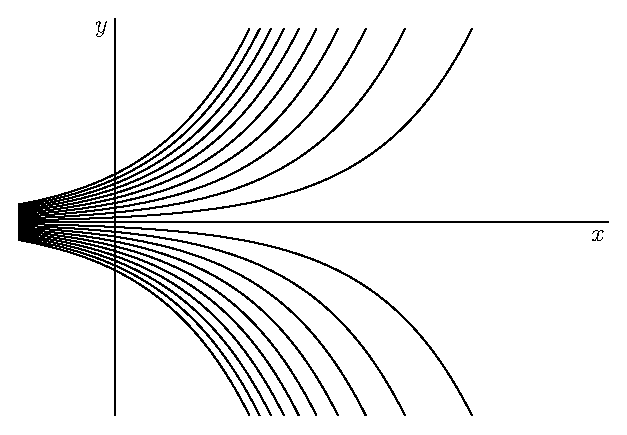
\includegraphics[width=8cm]{figure01.eps}
\caption{The family $f(t) = ce^{\alpha t}$ where $c \in \RR$.}
\label{figure-family-of-solutions}
\end{figure}

\begin{example}
The simplest differential equation is 
\begin{equation*}
\frac{df}{dt} = \alpha f(t).
\end{equation*}
For many differential equations, we seek a translation of their
meaning. This simple equation means the rate of change is
propotional to the current value. This is a statement of
percentage growth; the proportionality constant is the
percentage.
\end{example}

The solutions to this equation are are $f(t) = ce^{\alpha t}$.
Notice that there is a constant, $c$, such that there will be
a whole infinite family of solutions. A specific solution is
specified by a choice of $c$. 

Percentage growth applies to population models.
If this is the case, then $f(0) = ce^0 = c$ and we must
interpret the constant $c$ as the population when $t=0$.
If this is our starting point, we consider $c$ the
\emph{initial value} of the solution. A full solution of a
differential equation will usually consist of a function and
choice(s) for the initial value(s). 

\begin{defn}
A differential equation along with a specified initial value
is called an \emph{initial value problem} or IVP.
\end{defn}

If we don't make a choice, as we said, we get an infinite
family of solutions. We can visualize this family as a series
of graphs in $\RR^2$. Figure \ref{figure-family-of-solutions} shows
the graphs for $f(t) = ce^{\alpha t}$. 

\subsection{Pure and Applied Perspectives}
\label{pure-and-applied}

We will be looking at differential equation both from a pure
mathematics and applied mathematics point of view. The pure
mathematician is interested in these kinds of questions:

\begin{itemize}
\item When does a solution exists?
\item Can we prove that a solution exists?
\item Is the solution unique?
\item Is there a complete family? How many parameters exist, and 
what are their domains?
\item Can we write and prove theorems to answer these questions?
\end{itemize}

The applied mathematician is interested in these kinds of
questions:

\begin{itemize}
\item How many solutions fit the data or initial values?
\item How do the solutions grow? What is their behaviour?
\item Are the solutiosnts stable?
\item How difficult are the solutions to calculate? Can we get
them exacly, or only approximately?
\item Can we answer questions about the model even without a
solution?
\end{itemize}

\subsection{Interesting Examples}
\label{interesting-examples}

We want to know the behaviour of solutions of DEs. Several
examples in this section give the lay of the land.

\begin{example}
\begin{equation*}
\frac{d^2f}{dt^2} + 9 f = 0
\end{equation*}
This is solved by $\sin 3t$ and also by $\cos 3t$. Moreover, any
linear combination $a\sin 3t + b \cos 3t$ is a solution. 
In a second order equation, we often expect two linearly
independent solutions and the general solution is a linear
combination of the two linearly independent solutions.
\end{example}

\begin{example}
\begin{equation*}
\frac{dy}{dt} = t \sqrt{y}
\end{equation*}
This is solved by $y = (\frac{t^2}{4} + c)^2$, which is a nice
family with one real parameter. However, this is also solved
by $y=0$, even though it isn't in the family. 
\end{example}

\begin{defn}
An extraneous solutions to a DE, one which fall outside
families with parameters, is called \emph{singular solution}.
\end{defn}

\begin{example}
\begin{equation*}
t \frac{dy}{dt} = 4y 
\end{equation*}
This is solved by $y = ct^4$, which is another reasonable
family. However, there is a strange, singular solution.
\begin{equation*}
y(t) = \left\{ \begin{matrix} -t^4 & t \leq 0 \\ t^4 & t>0
\end{matrix} \right.
\end{equation*}
The derivatives of this function line up at the origin, so the
function is of class $C^1$ (actually $C^3$, if you work it
out).  
\end{example}

\begin{example}
\begin{equation*}
\frac{dy}{dx} = \frac{-x}{y} 
\end{equation*}
The curve $x^2 + y^2 = c$ solves this equation implicitly.
We could break this up into two functions, but its much more
natural to leave it as an implicit locus, in this case, a
circle. This is very typical: often solutions are left in an
implicit form as loci, even though in theory we
always look for functions $y = f(x)$. Also notice in this
example that only non-negative $c$ values are allowed
in this family of solutions. There is no guarantee that all
values of a parameter will lead to reasonable solutions.
\end{example}

\subsection{The Pessimistic Outlook}
\label{pessimism}

In some sense, a DE is an mathematical application of the
scientific method. Often an observation about a phenomenon can
be expressed as a relationship between a function and its
derivative, such as the observation of percentage growth. The
DE, then, is the hypothesis born of observation. If we can
find the solution, it gives us a predictive model of the
phenomenon, which we can test. If the solution matches the
observed behaviour, we conclude the DE model is relatively
reliable; if the solution diverges from the observed
behaviour, we discard or amend the DE.

In this way, DEs allow the modelling many phenomena:
popluations, radioactive decay, cooling, disease, 
metabolish, newtonian motion with friction, chemical
reactions, gravity, predaor-prey models, hamiltonian
mechanics, quantum mechanics, interest, bacterial growth,
neuron firing, ecology, mixtures, draining, series
circuits, suspended cables, and many, many more.

However, for all this power and utility, DEs are terribly
difficult to solve. The sad truth is that we can exactly
solve only a very small portion of them. Due to this
limitation, many techniques are developed to understand
approximate solutions or infer information about solutions
indirectly.

In addition, many DEs have solutions which are entirely new
functions. 

\begin{example} 
\begin{equation*}
\frac{dy}{dt} = e^{-t^2} \implies y = \int e^{-t^2}dt + C
\end{equation*}
This integrand is a $C^\infty$ function, so the
anti-derivative exists, but there is no name for it in the
elementary functions. This is not uncommon. Often we will
`solve' a differential equation by simply naming the solution
with a new name, since it is an entirely new function.
\end{example}

\section{Qualitative Methods for First Order DEs}
\label{qualitative-methods}

As we said before, many DEs are very difficult or impossible
to solve directly. Implicit or qualitative methods try to say
something about the solutions without actually finding the
solutions. Even when we can exactly solve an equation, these
methods are great for interpreting the behaviour of the
solutions.

\subsection{Autonomous DEs and Phase-Line Analysis}
\label{phase-line}

Consider a population model $p(t)$ with its autonomous DE.
\begin{equation*}
\frac{dp}{dt} = f(p)
\end{equation*}
There is a lovely piece of qualitative analysis for
autonomous equations called the \emph{phase line analysis}.
Phase line analysis looks at the right side of the equation
and asks: what values of $p$ set the right side to
zero. What does this mean? When the right side of our
differential equation is 0, the left side is 0 as well.
The left side is the growth rate, so that means the growth
rate is zero. This is a value of the population
$p$ where there is no growth. 

\begin{defn}
In an autonomous DE, a value of the
function where the derivative vanishes is called a 
\emph{steady states}
\end{defn}

If the population is
exactly at its steady state, it will not change; steady states
are constant populations which do no grow or decline. (For
population models, we can make the reasonable assumptions that
$p \geq 0$ and $p=0$ is always a steady state. Otherwise, we
can have any real values on the phase line.)

Once we have the steady states, we ask what happens between
each steady state. Assuming that the DE is reasonable, then
between the steady states, the right side will be either
positive or negative. When it is positive, we have a positive
growth rate and the population increases. When it is
negative, we have a negative growth rate and the population
decreases. 

\begin{defn}
In an autonomous DE, the direction of growth negative or
positive, called the \emph{trajectory} of the popluation.
\end{defn}

Steady states and trajectories give us an
remarkably complete understanding of the population.
\begin{smallitemize}
\item If the popluation is at a steady state, it doesn't
change.
\item If the popluation is not at a steady state, we look at
the trajectory.
\item If the trajectory is positive, the popluation grows
either to the closest larger steady state or to infinity.
\item If the trajectory is neagative, the population declines
either to the closest smaller steady state or to zero.
\end{smallitemize}

We summarize this information is a phase line diagram. We
take a ray representing $p \geq 0$ and put dots on the ray for
the steady states. In between, we put arrows to show the
trajectories. Its best to see the phase line diagrams through
examples.

\begin{figure}[t]
\centering
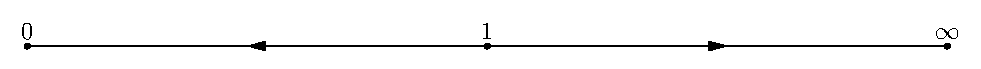
\includegraphics[width=12cm]{figure02.eps}
\caption{A Phase Line Diagram for $\frac{dp}{dt} = p^2 - p$}
\label{figure-phase-line1}
\end{figure}

\begin{figure}[t]
\centering
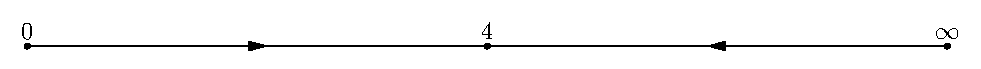
\includegraphics[width=12cm]{figure03.eps}
\caption{The Logistic Phase-Line Diagram}
\label{figure-logistic-phase-line}
\end{figure}

\begin{example}
\begin{example}
\begin{equation*}
\frac{dp}{dt} = p^2 - p
\end{equation*}
The right side is zero when $p=0$ or $p=1$, so those are the
steady states. When $p \in (0,1)$ the derivative is negative,
so the trajectory is decreasing. When $p \in (1, \infty)$, the
derivative is positive, so the trajectory is increasing.
Figure \ref{figure-phase-line1} shows the resulting
phase-line.
\end{example}

This example is a specific instance of a form known as the
logistic equation.
\begin{equation*}
\frac{dp}{dt} = 4p-p^2
\end{equation*}
The right side is zero when $p=0$ or $p=4$, so those are the
steady states. When $p \in (0,4)$ the derivative is positive,
so the trajectory is increasing. When $p \in (4, \infty)$, the
derivative is negative, so the trajectory is decreasing.
Figure \ref{figure-logistic-phase-line} shows the resulting
phase-line.
\end{example}

\begin{figure}[t]
\centering
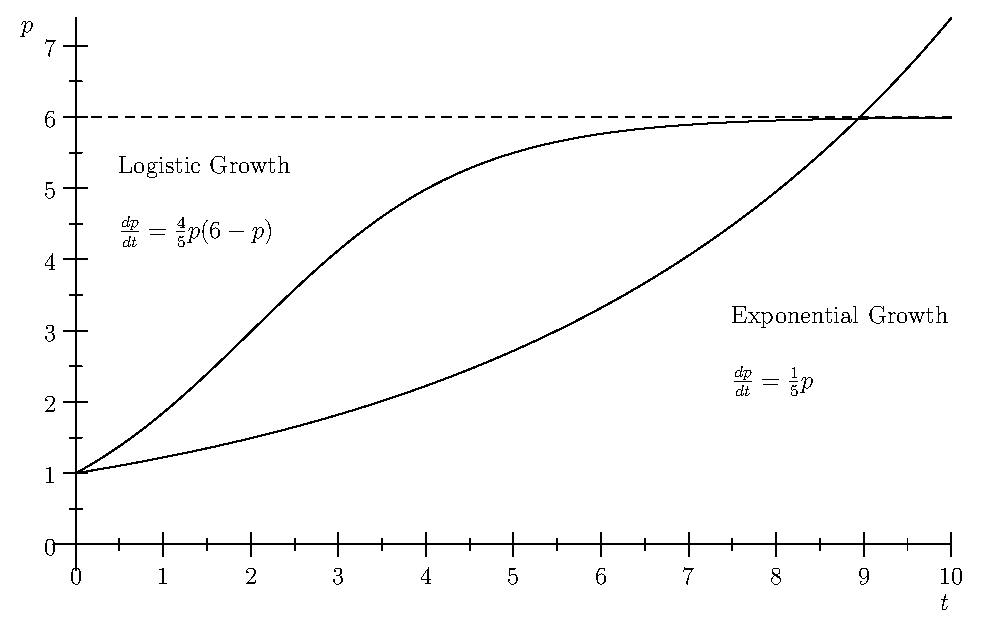
\includegraphics[width=12cm]{figure04.eps}
\caption{Exponential and Logistic Growth}
\label{figure-exponential-growth}
\end{figure}

The logistic equation leads to logistic growth. We can see
from the phase line diagram that the trajectories all point
towards the value $p=4$. In logistic growth, the values
always want to revert to some non-zero steady state. From
below, this is growth up to some firm maximum. After
exponential growth, logistic growth is the most commonly used
model for populations. Figure \ref{figure-exponential-growth} shows
both exponential and logistic growth (where the steady state for the
logistic model is at $p=6$.)

\begin{figure}[t]
\centering
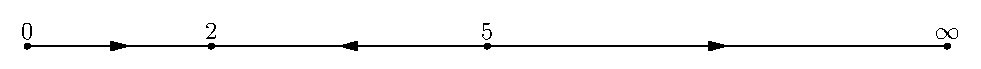
\includegraphics[width=12cm]{figure05.eps}
\caption{A Phase Line Diagram}
\label{figure-phase-line2}
\end{figure}

\begin{example}
\begin{equation*}
\frac{dp}{dt} = p^3 -7p^2 + 10p
\end{equation*}
The right side factors as $p(p-2)(p-5)$, so it is zero then
$p=0$, $p=2$ or $p=5$. Those are the
steady states. When $p \in (0,4)$ the derivative is positive,
so the trajectory is increasing. When $f \in (2,5)$, the
derivative is negative, so the trajectory is decreasing. When
$p \in (5,\infty)$, the derivative is positive, so the
trajectory is increasing. Figure \ref{figure-phase-line2}
shows the phase line.
\end{example}

\subsection{Direction Fields}
\label{direction-fields}

If the equation is not autonomous, then the phase-line is too
simple a tool to capture the details. However, if we can
solve for the derivative, we can write a first order DE as
\begin{equation*}
\frac{dy}{dx} = F(x,y).
\end{equation*}
This allows a very useful interpretation: the left side is the
slope of a graph, the right side is a function on $\RR^2$,
giving a value at every point in the plane. Together, we
determine a slope at every point in the plane. 

\begin{defn}
A determination of a slope at all point in a subset $U$ of
$RR^2$ is called a \emph{direction field}.
\end{defn}

\begin{figure}[t]
\centering
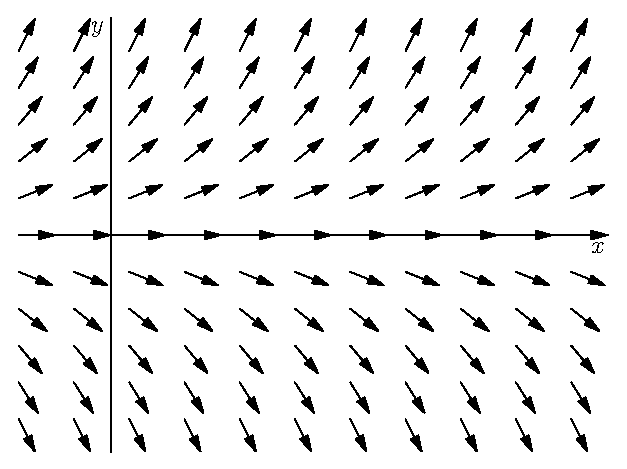
\includegraphics[width=6cm]{figure06.eps}
\caption{The Direction Field for $\frac{dy}{dx} = y$.}
\label{figure-direction-field1}
\end{figure}

\begin{figure}[t]
\centering
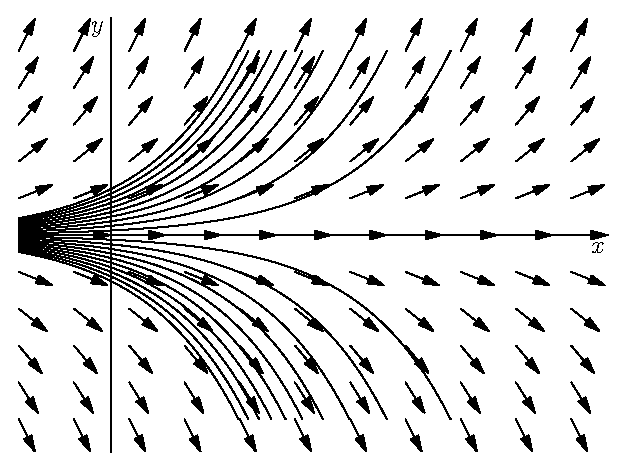
\includegraphics[width=6cm]{figure07.eps}
\caption{The Integral Curves for $\frac{dy}{dx} = y$.}
\label{figure-direction-field1-curves}
\end{figure}

If there are solutions to the DE, then they must be functions
which fit these slopes. Therefore, the slopes give us a sense
of what the functions look like. Let's go back to the
simplest example.

\begin{example}
\begin{equation*}
\frac{dy}{dx} = y
\end{equation*}
The slope at a point $(x,y)$ is $y$, so the slope at $(3,4)$
is $4$, the slope at $(-2,-3)$ is $-3$ and the slope at
$(32,0)$ is $0$. Figure \ref{figure-direction-field1} shows the
direction field.

The solutions exactly fit the direction field.
Therefore, if we can draw and understand the direction field,
we get a sense of the solutions. Notice that since the
direction field fills $\RR^2$ (or a portion of it), we expect
an infinite family of graphs of functions to match all the
slopes. Figure \ref{figure-direction-field1} shows the
graphs of the infinite family of solutions.
\end{example}

Let's go back to the strange examples in the previous section
and draw their direction fields.

\begin{figure}[t]
\centering
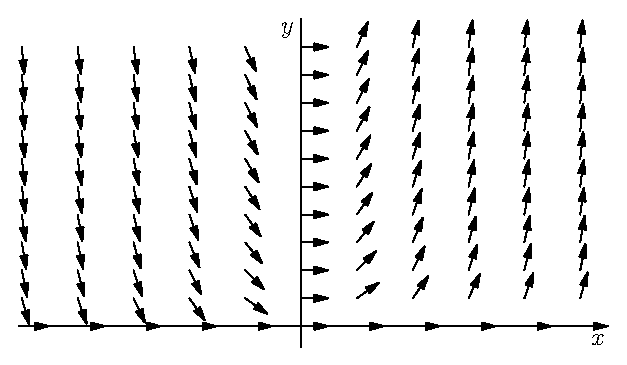
\includegraphics[width=9cm]{figure08.eps}
\caption{The Direction Field for $\frac{dy}{dx} = x \sqrt{y}$.}
\label{figure-direction-field2}
\end{figure}

\begin{figure}[t]
\centering
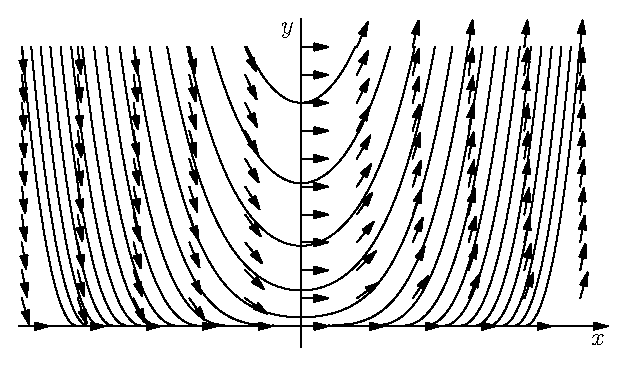
\includegraphics[width=9cm]{figure09.eps}
\caption{The Integral Curves for $\frac{dy}{dx} = x \sqrt{y}$.}
\label{figure-direction-field2-curves}
\end{figure}

\begin{example}
\begin{equation*}
\frac{dy}{dx} = x \sqrt{y}
\end{equation*}
Figure \ref{figure-direction-field2} shows the direction field
and the infinite family of solutions.  We see the entire
family $y = (\frac{x^2}{4} + c)^2$, but we also see the
singular solution $y=0$. 
\end{example}

\begin{figure}[t]
\centering
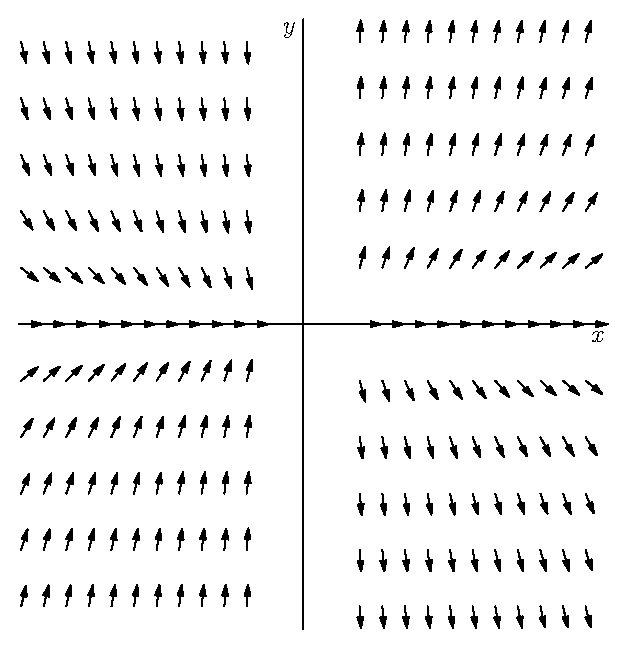
\includegraphics[width=6cm]{figure10.eps}
\caption{The Direction Field for $\frac{dy}{dx} = \frac{4y}{x}$.}
\label{figure-direction-field3}
\end{figure}

\begin{figure}[t]
\centering
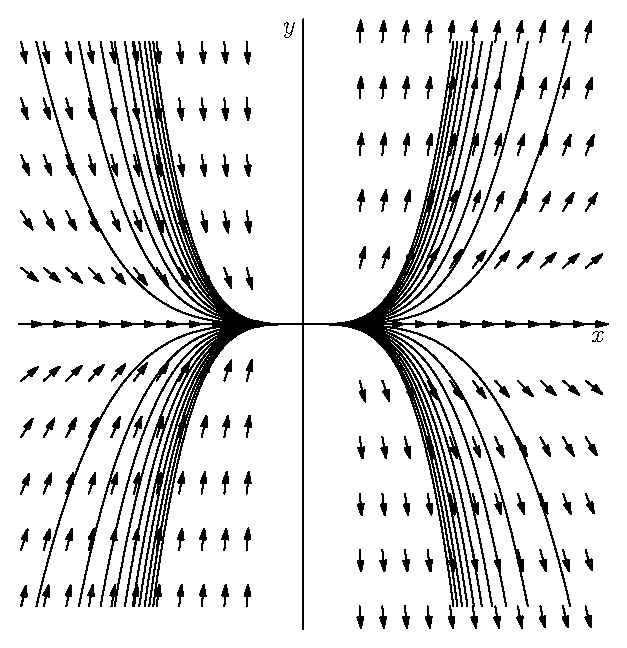
\includegraphics[width=6cm]{figure11.eps}
\caption{The Integral Curves for $\frac{dy}{dx} = \frac{4y}{x}$.}
\label{figure-direction-field3-curves}
\end{figure}

\begin{example}
\begin{equation*}
\frac{dy}{dx} = \frac{4y}{x}
\end{equation*}
There family of solutions $y = cx^4$ which fits the direction
field. The singular solutions are put together from one positive and
one negative piece. Figure \ref{figure-direction-field3} shows
the direction field and the infinite family of solutions.  
\end{example}

\begin{figure}[t]
\centering
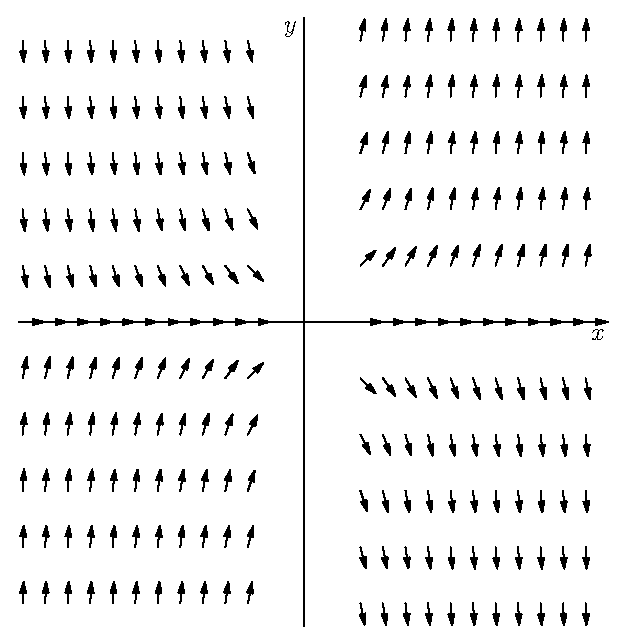
\includegraphics[width=6cm]{figure12.eps}
\caption{The Direction Field for $\frac{dy}{dx} = xy$.}
\label{figure-direction-field4}
\end{figure}

\begin{figure}[t]
\centering
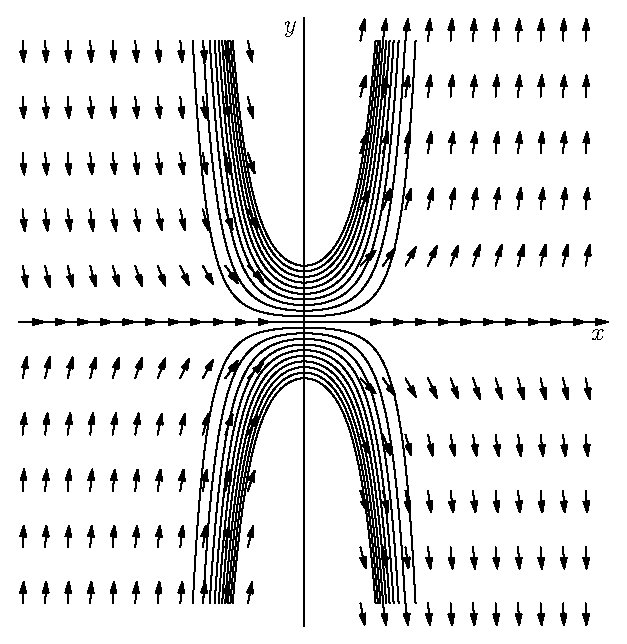
\includegraphics[width=6cm]{figure13.eps}
\caption{The Integral Curves for $\frac{dy}{dx} = xy$.}
\label{figure-direction-field4-curves}
\end{figure}

\begin{example}
\begin{equation*}
\frac{dy}{dx} = xy
\end{equation*}
This is solved by $y = ce^{x^2}$, including $c=0$ for $y=0$ as
a trivial solution. The direction field also shows the
stability behaviour of the function: in this case, the
functions grows very quickly away from the origin except for
the stable and trivial $y=0$ solution.  Figure
\ref{figure-direction-field4} shows the direction field and the infinite
family of solutions.
\end{example}

\begin{figure}[t]
\centering
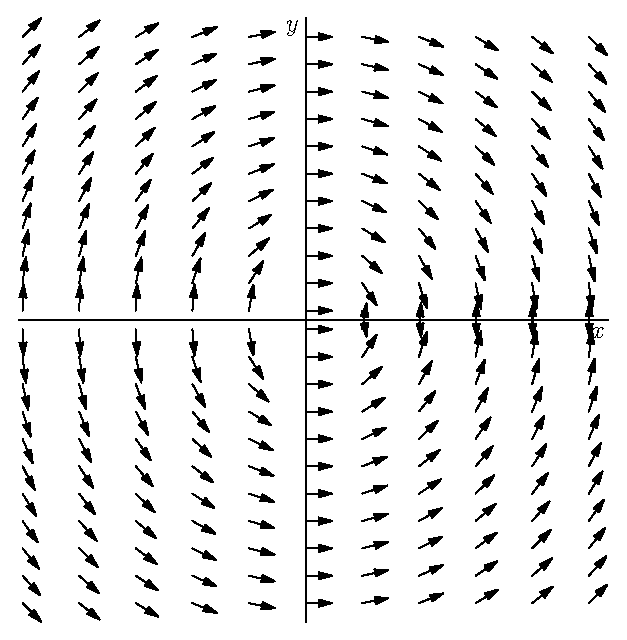
\includegraphics[width=6cm]{figure14.eps}
\caption{The Direction Field for $\frac{dy}{dx} = \frac{x}{y}$.}
\label{figure-direction-field5}
\end{figure}

\begin{figure}[t]
\centering
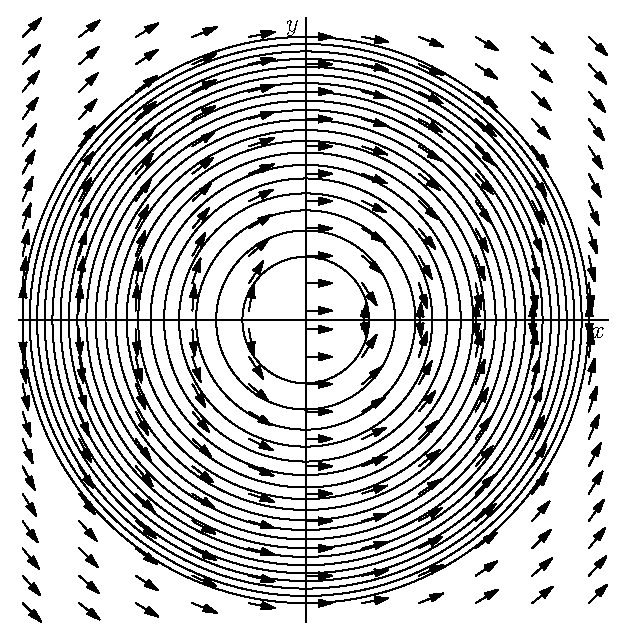
\includegraphics[width=6cm]{figure15.eps}
\caption{The Integral Curves for $\frac{dy}{dx} = \frac{x}{y}$.}
\label{figure-direction-field5-curves}
\end{figure}

\begin{example}
\begin{equation*}
\frac{dy}{dx} = -\frac{x}{y}
\end{equation*}
This is solved by $y = \pm \sqrt{c-x^2}$, which gives a series
of circles. The direction field shows the bounded, relatively
stable behaviour which is confirmed by the solutions. Notice
that these solution have finite domains: we are not guaranteed
solutions that apply to all real numbers. Figure
\ref{figure-direction-field5} shows the direction field and the infinite
family of solutions.
\end{example}

\section{Stability and Linearization}
\label{stability-and-linearization}

\subsection{Stability}
\label{stability}

Coming from applied mathematics, the language of stability is
a very useful language for talking about DEs. We again think
of a general autonomous DE as a population model.
\begin{equation*}
\frac{dp}{dt} = f(p)
\end{equation*}
We defined steady states when we did phase-line analysis:
these were roots of the function $f(p)$ and hence values of
$p$ where the rate of change is zero. 

\begin{defn}
The steady states of an autonomous DE are classified by their
\emph{stability} A steady state $P$ is \emph{stable} if $p(t)
\rightarrow P$ when the initial value is close to $P$. We can
also call these steady states \emph{attractors}. In the phase
line diagram, the trajectories points toward such states.
Similar, we can call a steady state \emph{stable or attractive
from above or below} if only one of the trajectories points
towards the steady state. If both trajectories point away, the
steady state is \emph{unstable}.
\end{defn}

\subsection{Linearization}
\label{linearization}

Once we have identified a steady state of a DE system, we
often are only interested in the behaviour of slight
perterbations from the steady state. This is the behaviour
that stability capture: whether we approach or diverge from
the steady state when we start a small distance away. If
$P$ is a steady state, the we can define a new function $q(t)
= p(t) - P$. A change of variables results in 
\begin{equation*}
\frac{dq}{dt} = f(P + q).
\end{equation*}
If we expand $f$ as a taylor series centered at $p$, this becomes
\begin{equation*}
\frac{dq}{dt} = f(P + q) = f(P) + f^\prime(P) (P+q -P) +
\ldots = f^\prime(P) q + \ldots.
\end{equation*}

\begin{defn}
The \emph{linearization} of the DE at the steady state $P$ is
\begin{equation*}
\frac{dq}{dt} = f^\prime(P) q.
\end{equation*}
\end{defn}

The solution to the linearized DE is 
\begin{equation*}
q(t) = q_0 e^{f^\prime(P) t}.
\end{equation*}
In particular, this linearized solution is either
exponential growth or decay, depending on the sign of
$f^\prime(P)$. Therefore, the sign of $f^\prime(P)$
determines the stability: positive and the solution is
unstabe, negative and the solution is stable. This can also
be seen in the phase line, since the sign of the derivative
can indicate the trajectories on either side of the steady
state. If $f^\prime(P) = 0$, then the stability is determined
by the higher order terms of the taylor series expansion.

For now, there isn't much more we will do with this
linearization. However, it is worth introducing here as a
theme since it is so central to applied mathematics. Linear
equations are almost always the first kind of DE that we try
to use, typically since they have elegant and accessible
solutions. Everything else gets simply referred to a
`non-linear'; in many ways, `non-linear' is a synonmy for
annoying and complication. However, linear models only go so
far and often the non-linearity holds the key to understanding
a model. Even so, we will often try to understand the
linear part and then figure out how to add in the
non-linearity in a reasonable fashion to add subtleties to
various models. 

\section{Seperable Equations}
\label{seperable-des}

\begin{defn}
A \emph{seperable equation} is a DE which has the form 
\begin{equation*}
\frac{dy}{dt} = f(y) g(t).
\end{equation*}
\end{defn}

The method of solving seperable equations treats the $dt$ and
$dy$ terms as independent infinitesimals, a strange but
historically reasonable treatment. If we allow for these
independent infinitesimals, we can seperate (hence the name)
the DE into two pieces, one involving each variable.
\begin{equation*}
\frac{1}{f(y)} dy = g(t) dt 
\end{equation*}
Then, again acting somewhat strangely by modern notational
conventions, we integrate both sides with respect to their own
variables.
\begin{equation*}
\int \frac{1}{f(y)} dy = \int g(t) dt
\end{equation*}
The solution is then left implicit unless we can reasonable
solve for $y$, in which case we can write $y$ as a
conventional function of $t$.

If you are interested in the justification of this splitting
procedure, we could think of the operation alternatively,
writing $f(y(t))$ to remember the independent variable. If
we bring the $f(y)$ to the left side, we get the expression
\begin{equation*}
\frac{1}{f(y(t))} \frac{dy}{dt} = g(t).
\end{equation*}
Then we can integrate both sides with respect to $t$, which is
a reasonable and justified operation.
\begin{equation*}
\int \frac{1}{f(y(t))} \frac{dy}{dt} dt = \int g(t) dt
\end{equation*}
Finally, we change of variables from $t$ to $y$ in the left
side integral. 
\begin{equation*}
\int \frac{1}{f(y)} dy = \int g(t) dt
\end{equation*}
In theory, we should get two constants of integration, one
from each side. However, we can move the left side constant to
the ride side and have the difference of two arbitrary
constants, which is equivalent to one arbitrary constant.
Therefore, we will only write on constant of integration for
seperable equations. 

In general, mathematicians have a practice of being somewhat
careless with this constant. Since it doesn't need to be
determined until we use an initial condition, we often forgoe
various operations on the constant. For example, if we had
$2(t+c)$, we would often simplify this to $2t+c$, since
whether we figure out the constant from $c$ or from $2c$
later, its value is still determined by the initial condition.
It's useful to become accustomed to this carelessness
constants of integration.


\begin{example}
\begin{align*}
\frac{dy}{dx} & = \frac{\sin x}{y} \\
y dy & = \sin x dx \\
\frac{y^2}{2} & = - \cos x + c \\
y & = \pm \sqrt{c - 2\cos x}
\end{align*}
It is interesting to note where the constant of integration ends
up. Since integration isn't the final step (we have to also
solve for $y$), the constant moves around in the resulting
algebra. In DE, we can't just add $+c$ at the very end of the
process.

\begin{figure}[t]
\centering
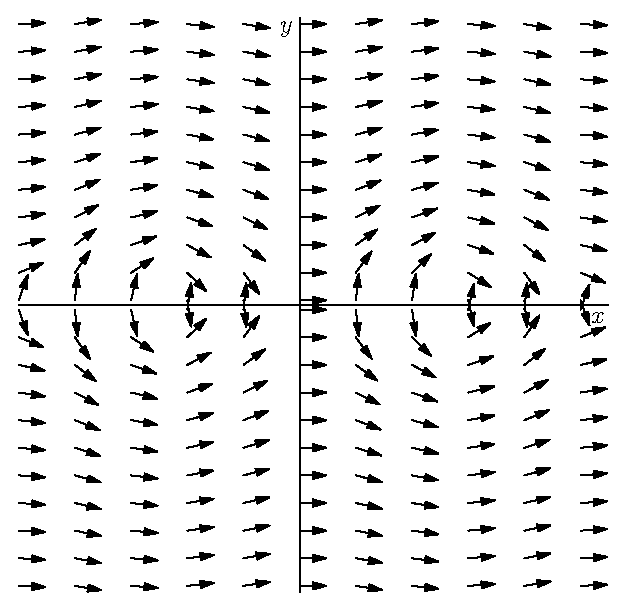
\includegraphics[width=6cm]{figure16.eps}
\caption{Direction Field for $\frac{dy}{dx}= \frac{\sin x}{y}$}
\label{figure-direction-field6}
\end{figure}

\begin{figure}[t]
\centering
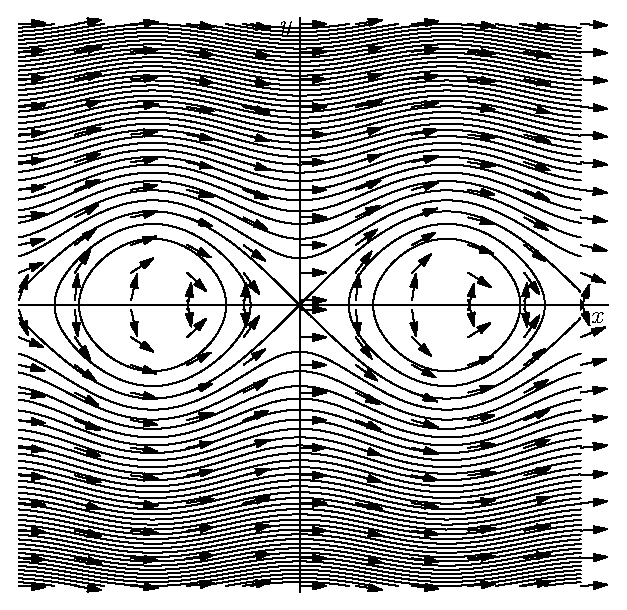
\includegraphics[width=6cm]{figure17.eps}
\caption{Direction Field with Solutions for $\frac{dy}{dx}=
\frac{\sin x}{y}$}
\label{figure-direction-field8}
\end{figure}

If we impose an initial condition of $y(0) = 1$, we can
determined the value of the constant of integration.
\begin{align*}
1 & = \sqrt{c - 2 \cos (0)} = \sqrt{c-2}\\
1 & = c-2 \\
c & = 3 \\
y & = \sqrt{3 - 2 \cos x} 
\end{align*}
\end{example}

Figure \ref{figure-direction-field6} shows the direction
field and solution for this example.  Notice the strange
domain issues with this implicit plot. When $|c| \leq 2$, we
have restricted domain solutions, represented by the closed
curves. There are no solutions at all when $c < -2$. We have
solutions with domain $\RR$ only for $c \geq 2$. When $c = 2$,
we get the strange crossed graph, which is not always
differentiable. When $c=-2$. the ``solution'' is only defined
at discrete points.

\begin{figure}[t]
\centering
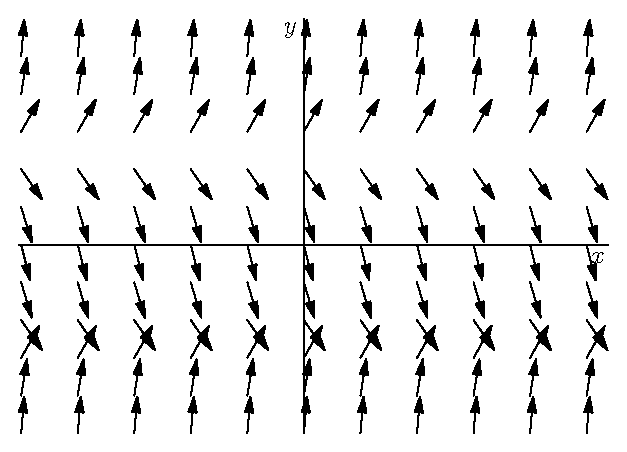
\includegraphics[width=6cm]{figure18.eps}
\caption{The Direction Field for $\frac{dy}{dx} = y^2-4$.}
\label{figure-direction-field7}
\end{figure}

\begin{figure}[t]
\centering
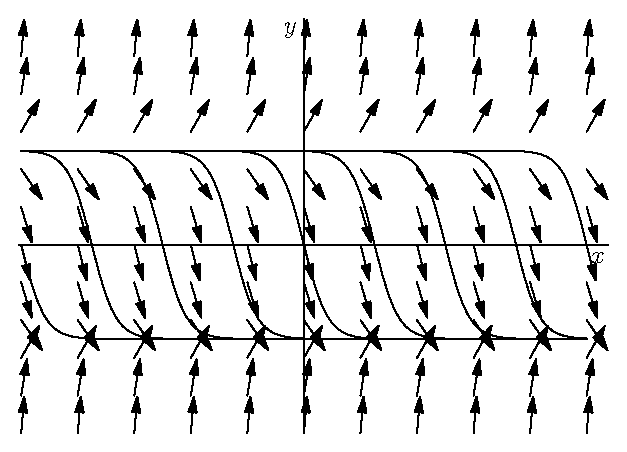
\includegraphics[width=6cm]{figure19.eps}
\caption{The Integral Curves for $\frac{dy}{dx} = y^2-4$.}
\label{figure-direction-field7-curves}
\end{figure}

\begin{example}
This is an autonomous example.
\begin{align*}
\frac{dy}{dx} & = y^2 - 4 \\
\int \frac{1}{y^2-4} dy & = \int 1 dx \\
\frac{-1}{2} \arctanh \left( \frac{y}{2} \right) & = x + c \\
\arctanh \left( \frac{y}{2} \right) & = -2x + c \\
\frac{y}{2} & = \tanh (-2x + c) \\
y & = 2 \tanh (-2x + c) \\
\end{align*}
Since this is an autonomous equation, we can look for steady
(constant) singular solutions when the right side of the
equation vanishes. Here, $y=2$ and $y=-2$ are steady states.
Moreover, $y=2$ is stable and $y=-2$ is unstable.
This can be seen in the direction field and implicit plot in
Figure \ref{figure-direction-field7} 

It is also interesting to note that the
output of $\tanh$ is only $-1$ to $1$, so it is 
impossible to get $y \leq -2$ or $y \geq 2$. We should
wonder if there are solutions in this range at all. In the
implicit plot, we could draw curves with these $y$ values.
These other curves are found by doing the integral
differently, since both hyperbolic tangent and hyperbolic
cotangent have the same anti-derivative. $y=2 \coth (-2x +
c)$ is also a solution.
\end{example}

\section{Existence and Uniqueness of Solutions}
\label{existence-and-uniqueness}

Before moving on with other techniques for solving first order
equations, this is a nice place to take a pure-mathematical
detour and talk about existence and uniqueness of solutions.
We're going to deal with first order equations where we can
isolate the derivative term, that is, equations of the form
\begin{equation*}
\frac{dy}{dx} = F(x,y).
\end{equation*}
The details of existence and uniqueness theorems rely on the
properties of $F$ as a function of two variable. In this
treatment, we think of $y$ and $x$ as two unrelated,
independent variables, even though the DE itself implies that
$y$ is a function of $x$.

\subsection{Existence}
\label{existence}

Existence of solutions to first order DES is established by
the Peano Existence Theorem. 

\begin{thm}
In a equation of this form above, if $F$ is continuous in both variables
in an open set $U \subset \RR^2$ and if $(x_0,y_0) \in U$,
then there exists $\epsilon > 0$ such that the Initial Value
Problem associated to the DE and the initial condition $y(x_0)
= y_0$ has a solution with domain at least
$[x_0-\epsilon,x_0+\epsilon]$. 
\end{thm}

This is a very local result: the small positive $\epsilon$
only guarantees a tiny piece of a function as a solution.
Existence (and later uniqueness) are only guaranteed very
close to the initial value of the function. We do know that
the function is differentiable in this small inteval, but we
don't know anything else: outside the interval, anything could
happen with the solution.

It's also useful to note, particularly for students with
experience in other senior mathematics classes, that this
theorem relies on topological considerations: we need an open
subset $U$ where $F$ is continuous.

\begin{example}
\begin{equation*}
y^\prime = y^{\frac{2}{3}} \hspace{2cm} y(0)=0
\end{equation*}
This satisfies the conditions of the theorem, so a solutions
exists. However, there are two solutions: $y=0$ and
$y=x^3/27$. Peano's theorem doesn't imply the uniqueness of a
solution.
\end{example}

\begin{example}
\begin{equation*}
y^\prime = \sqrt{|y|} \hspace{2cm} y(0) = 0
\end{equation*}
This $F$ is also continuous near $(0,0)$, so a solution exists
by Peano's theorm. This IVP is solved by $y=0$ and $y =
x^2/4$. It's obvious that we need something more to ensure
uniqueness.
\end{example}

Before we move on to the next result, we could ask for the
proof of this theorem. Unforunately, that proof doesn't fall
within the scope of this course. We would need to establish a
number of new definitions and techniques from real analysis,
as well as struggle through a bunch of tricky $\epsilon$ and
$\delta$ arguments. It's interesting stuff, but very
challenging and therefore left aside for this course.

\subsection{Lipschitz Continuity}
\label{lipschitz}

In order to state the theorem about uniqueness, we need a new
definition of continuity. 

\begin{defn}
A function from an open set $U$ in
$\RR$ to $\RR$ is called \emph{Lipschitz continuous} if
$\exists K > 0$ such that $\forall x_1,x_2 \in U$ we have
$|f(x_1) - f(x_2)| \leq K|x_1-x_2|$.
\end{defn}

This is a strange kind of continuity. The definition is
stronger than normal: Lipschitz continuity implies
normal continuity. Moreover, the definition is global over
$U$, not just local like conventional continuity. Therefore,
the domain matters: a function might be Lipschitz continuous
on a small set, but not on a larger one. 

As an interpretation, Lipschitz continuity is a control on the
global growth over the designated set. For a Lipschitz
continuous function, there is a linear function that bounds
the function on the designated set. Unsurprisingly, this means
that the defintion usually only works on bounded sets.
As a visualization, we can think of the definition as
comparing $f$ to a function $g(x) = K|x|$. The graph of $g$
gives a cone in $\RR^2$ and the $f$ must stay inside this cone
to be Lipschitz continuous. In this way, the definition 
limits the local growth of $f$ and its derivatives.

\begin{example}
Here are some examples to illustrate the idea of Lipschitz
continuity.
\begin{smallitemize}
\item $f(x) = x$ is Lipschitz continuous for $K=1$ on any interval,
since it is bounded by itself, a linear function. 
\item $f(x) = x^2$ is Lipschitz continuous on any \emph{bounded}
interval. Specifically, on $(-7,7)$ we can take $K=14$.
However, $f(x) = x^2$ is not Lipschitz continuous on all of
$\RR$, since no linear function bounds it. 
\item $f(x) = x^{\frac{2}{3}}$ is not Lipschitz continuous on
$(-1,1)$, since its slope gets arbitrarily steep near the
origin. This means that very close to $0$, it cannot be
bounded by a linear function through $(0,0)$. 
\end{smallitemize}
\end{example}

The previous example was not Lipschitz continuous at $0$, and
it also failed to be differentiable at that point. We might
wonder if differentiability is a sufficient condition. That
would be convenient, since we know how to check for
differentiability. However, consider a strange
example.

\begin{example}
\begin{equation*}
f(X) = \left\{ \begin{matrix} x^{\frac{3}{2}} \sin \left(
\frac{1}{x} \right) & x \in (0,1] \\ 0 & x = 0 \end{matrix}
\right. 
\end{equation*}
This isn't Lipschitz continuous, but it is differentiable near
zero, showing that differentiability isn't sufficient.
However, there is some good news: this example
is a strange aberation. 
\end{example}

\begin{prop}
A function which is $C^1$ at a point $a$ in its domain is also
Lipschitz continuous at a.
\end{prop}

$f \in C^1$ is roughly equivalent to saying that
$\frac{\del f}{\del y}$ must exist and be bounded. This last
criterion is the one we will use in practice: we check if the
derivatives exists and if it is bounded.

Consider the $f(x) = x^2$. The derivaitve is $2x$,
which is bounded locally near $0$. $f(x) = x^\frac{2}{3}$ has
derivative $\frac{2}{3} x^{\frac{-1}{3}}$ which is unbounded
near 0. The former function is Lipschitz continuous and the
later is not.

\subsection{Uniqueness}
\label{uniqueness}

The theorem for Uniqueness is called the Picard-Lindel\"of
thereom. It is a small improvement and adjustment of the
Peano existence theorem. 

\begin{thm}
If $F$ is Lipschitz continuous in y
and continuous is x on an open set $U$ in $\RR^2$ and if
$(x_0,y_0) \in U$ then the initial value problem
\begin{equation*}
\frac{dy}{dx} = F(x,y) \hspace{2cm} y(x_0) = y_0
\end{equation*}
has a unique solution $y=f(x)$ defined on the domain
$[x_0-\epsilon,x_0+\epsilon]$ for some $\epsilon > 0$. 
\end{thm}

All of the comments from the previous theorem apply here. The
result is very local, relies on topology, and the proof is
beyond the scope of the course.

\begin{example}
\begin{equation*}
\frac{dy}{dx} = x \sqrt{y}
\end{equation*}
We considered this differential equation earlier.  It had
multiple solutions for initial value $y(0) = 0$. The function
$F(x,y) = x\sqrt{y}$ has $y$ deriavtive $\frac{\del F}{\del y}
= \frac{x}{2\sqrt{y}}$, which is unbounded near $0$.
Therefore, it is not Lipschitz continuous and doesn't satisfy
the continious of the Picard-Lidenl\"of theorem, meaning that
we don't expect a unique solution.
\end{example}

Lastly, anticipating the next section, consider the general
first-order linear DE where $P$ and $Q$ are continuous
functions.
\begin{equation*}
\frac{dy}{dx} = Q(x) - P(x) y
\end{equation*}
In this case, $F(x,y) = Q(x) - P(x)y$ and the $y$ derivative
is $-P(x)$, which is bounded assuming that $F$ is continuous.
We can then apply the Picard-Lindel\"of theorem to conclude
that linear equations have unique solutions whenever their
coefficient functions $P$ and $Q$ are continuous.

\section{Linear Equations and Integrating Factors}
\label{linear-des}

First order linear equation have the general form
\begin{equation*}
a(t) \frac{dy}{dt} + b(t) y = f(t).
\end{equation*}
Here $a(t)$, $b(t)$ and $f(t)$ are various (usually continuous)
functions. If we avoid the values where $a(t) = 0$, we can divide
by $a(t)$ to isolate the derivative, giving the following
more typical form. (Remember the denominators! We
have to pay attention to the roots of $a(t)$
throughout the solution.)
\begin{equation*}
\frac{dy}{dt} + P(t) y = Q(t)
\end{equation*}

\subsection{Homogeneous Solutions}
\label{homogenoues}

The linear DE is called homogeneous if $Q(t) = 0$. In the
homogeneous case, the DE is relatively easy to solve as a
seperable equation.
\begin{align*}
\frac{dy}{dt} & = -P(t) y \\ 
\frac{1}{y} dy & = -P(t) dt \\
\int \frac{1}{y} dy & = -\int P(t) dt \\
\ln |y| & = -\int P(t) dt + c\\
y & = c e^{-\int P(t)} dt
\end{align*}
I should make a couple of notes about this calculation.
\begin{smallitemize} 
\item We are informal with the constant. When we take
exponents of each side of the equation, we should have
multiplication by $e^c$.  However, since this is still an
undetermined constant, we simply write $c$ instead of $e^c$.
Also, when we drop the absolute value bars from $y$, we should
have a $\pm$ term.  Again, since $c$ can be either positive or
negative, we don't worry about that $\pm$. 
\item We had a $y$ in the denominator for this process, which
means that we have to be careful at points where $y=0$. We use
limits to figure out behaviour when $y$ gets close to zero.
\item If $P$ is constant, this is our most basic exponential
equation with solution $y = ce^{-\alpha t}$.
\end{smallitemize}

\subsection{Linear Operators and Superposition}
\label{superposition}

Recall from Definition \ref{definition-linear-differential-operator}
the idea of linear operators. If we write $L = \frac{d}{dt} + P(t)$,
we can write a second order DE as
\begin{equation*}
L y = Q(t).
\end{equation*}
This is a \emph{linear} differential operator, so it behaves
linearly, that is, it has the two linearity properties.
\begin{align*}
L(y_1 + y_2) & = Ly_1 + Ly_2 \\
L(cy) & = cL(y) 
\end{align*}
Then consider both the homoegenous equation $Ly = 0$ and a
non-homogenous equation $Ly = Q(t)$. If $f$ is a solution to
the non-homogenous equation, then $Lf = Q(t)$, and if $g$ is a
solution to the homogenous equation, then $Lg = 0$. By
linearity, we can conclude that 
\begin{equation*}
L(f+\alpha g) = Lf + \alpha Lg = Q(t) + \alpha \cdot 0 = Q(t).
\end{equation*}

\begin{defn}
If we have a solution to $Ly=Q(t)$, we can get
other solutions by adding multiples of the solution to the
homogeneous equation $Ly=0$. The solution to $Ly = Q(t)$ is
called the \emph{particular solution} and this process is called
\emph{superposition of solutions}. 
\end{defn}

For those who remember their linear algebra, we can think of
the solutions of a linear equation as a linear subspace of the
vector space of differentiable functions (on an appropriate
domain). In this sense the solution set of a linear equation
is an offset span: the non-homogenous solution is the offset
and the basis of the span is any homogenous solution.
Superposition gives us the family-structure of solutions to
linear equations.  Any multiple of a homogenous solutions can
be added to the particular solution, so the family is the
particular solution plus any multiple of a homogeneous
solutions: $y_p + \alpha y_h$. This $\alpha$ is the parameter
of the family.

\subsection{Integrating Factors}
\label{integrating-factors}

We know how to solve homogenous linear equations, since they
are seperable. Finding non-homogenous solutions is
somewhat more difficult; since these are not seperable
equations, we need a new technique. 

Let $L = \frac{d}{dt} + Q(t)$ be as before, and let
$y_h$ be a homogeneous solutions (a solution to $Ly = 0$). The
technique we will use is called \emph{variation of
parameters}. This technique says we should look for a
particular solution of the type $y_p = g(t) y_h$. Assuming
that our solution has this special form, we have to try to
find this $g(t)$. In order to do that, we put $g(t) y_h$ into
the equation.
\begin{align*}
Ly_p(t) = L g(t) y(t) & = Q(t) \\
g^\prime(t) y(t) + g(t) y^\prime(t) + g(t) P(t) y(t) & = Q(t) \\
g^\prime(t) y(t) + g(t) \Big( y^\prime(t) + P(t) y(t)
\Big) = g^\prime(t) + g(t) L y & = Q(t) \\
g^\prime(t) y(t) + g(t) 0 & = Q(t) \\
g^\prime(t) & = \frac{Q(t)}{y(t)} \\
g(t) & = \int \frac{Q(t)}{y(t)} 
\end{align*}
We can put this back into our special form and use the fact
that the homogeneous solution is $y = e^{-\int P(t)dt}$.
\begin{align*}
y_p = g(t) y & = \left( \int \frac{Q(t)}{e^{-\int P(t) dt}} dt
\right) e^{-\int
P(t) dt } \\
y_p & = e^{-\int P(t) dt} \int e^{\int P(t) dt} Q(t) dt
\end{align*}

\begin{defn}
In solving a linear equation of the for $\frac{dy}{dt} + P(t)
y = Q(t)$, the expression $e^{\int P(t) dt}$ is called an
\emph{integrating factor} and it is typically written
$\mu(t)$. 
\end{defn}

We rearrange the expression using the integrating factor.
\begin{align*}
e^{\int P(t) y} y_p & = \int e^{\int P(t) dt} Q(t) dt \\
\frac{d}{dt} \left( e^{\int P(t) dt} y_p \right) & = e^{\int P(t)
dt} Q(t) \\
\frac{d}{dt} (\mu (t) y_p(t)) & = \mu (t) Q(t) \\
y_p & = \frac{\int \mu(t) Q(t) dt + c}{\mu (t)} 
\end{align*}
Multiplying by the integrating factor turns the $y_p^\prime(t)
+ P(t) y_p(t)$ side of the equation into a product rule
derivative, which we can just integrate to solve. The
integrating factor turns a linear equation into something that
can be directly solved by integration, hence the name. It is
best to remember the process this way: the original
DE becomes a product rule derivative problem by multiplying
both sides of the original DE by the integrating factor and
then isolating $y_p$. 

This variation of parameters is the first instance of a very
common approach to solving DEs. Often, working with no idea of
what kind of function we are looking for is simply too
open-ended and too difficult. Therefore, we make a reasonable
guess regarding the form of the solution. Here, that guess was
$y_p = g(t) y_h$ where $g(t)$ was some unknown function. Then
we put out special form back into the DE and try to find
specific information about the parameter or unknown
involved.

\subsection{Examples}
\label{linear-equations-examples}

\begin{example}
\label{linear-example1}
\begin{equation*}
\frac{dy}{dt} + \frac{y}{t} = 2e^t
\end{equation*}
Since there is a $t$ in the denominator, we must avoid $t=0$
in the domain of solutions. We first look for the homogeneous
solution.
\begin{equation*}
y_h(t) = ce^{-\int \frac{1}{t}} dt = ce^{-\ln |t|} = \frac{c}{t} 
\end{equation*}
Then the integrating factor is
\begin{equation*}
\mu(t) = e^{\int \frac{1}{t} dt } = e^{\ln |t|} = t.
\end{equation*}
We use the integrating factor to get a new DE.
\begin{align*}
\mu(t) \frac{dy}{dt} + \mu(t) \frac{y}{t} & = \mu(t) 2e^t\\
t \frac{dy}{dt} + t \frac{y}{t} & = t 2e^t\\
\frac{d}{dt} (t y) & = 2te^t \\
ty & = \int (2te^t) dt \\
ty & = 2(te^t - e^t) + c \\
y & = 2 \left( e^t - \frac{e^t}{t} \right) + \frac{c}{t}
\end{align*}
Notice that we actually get the the homogeneous pieces here
from the constant of integration, getting the whole linear
family. Also notice that $t=0$ is excluded from the domain.
\end{example}

\begin{example}
\begin{equation*}
(t^2-9) \frac{dy}{dt} + ty = 0 
\end{equation*}
This is just a homogeneous DE. We note that $t \neq \pm 3$ in the domain.
The solution to the homogeneous case is
\begin{equation*}
y = e^{-\int P(t) dt} = e^{-\int \frac{t}{t^2-9} dt} = e^{
- \frac{1}{2} \ln |t^2-9| + c} = \frac{c}{\sqrt{t^2-9}}.
\end{equation*}
We should be careful with the absolute value in $\ln |f(t)|$.
The calculation can be done in two pieces, when $f(t) > 0$
and when $f(t) < 0$. In the previous calculation, we were a
little careless with this detail.
\end{example}

\begin{example}
\begin{equation*}
\frac{dy}{dt} + y = f(t)
\end{equation*}
To add some complication, the non-homogeneous function here
is going to be a step function.
\begin{equation*}
f(t) = \left\{ \begin{matrix} 1 & 0 \leq t \leq 1 \\ 0 & t > 1
\end{matrix} \right. 
\end{equation*}
This is still allowed: often the coefficients and functions
involved in DEs are only piecewise continuous and/or piecewise
differentiable. We can still work with them. The integrating
factor is $\mu(t) = e^{\int 1 dt} = e^t$.  We have to work
with two different intervals. First look at  $[0,1]$.
\begin{equation*}
\frac{d}{dt} e^t y = e^t \implies e^ty = e^t + c_1 \implies y = 1
+ c_1e^{-t} 
\end{equation*}
Alternatively, look at $(1,\infty)$.
\begin{equation*}
\frac{d}{dt} e^t y = 0 \implies e^ty = t + c_2 \implies y =
c_2e^{-t} 
\end{equation*}
We have two constants, but we want a continuous solution.
(It will fail to be differentiable at $t=1$, but that's alright.
There is a sudden change in the situation, so that's expected.)
Continuity at $1$ means that $e-c_1 = c_2$. The final
solution is a continuous piecewise function.
\begin{equation*}
y = \left\{ \begin{matrix} 1 - ce^{-t} & t \in [0,1] \\
(e-c)e^{-t} & t \in (1,\infty) \end{matrix} \right.
\end{equation*}
Even with this piecewise function, we can still do initial
value problems. If $y(0) =0$, we find
that $c=1$ and we get a specific solution.
\end{example}

\section{Substitutions}
\label{substitutions}

The third and final technique we will study for first order
DEs is substitution. At some level, solving DEs is a more
complicated and involved version of doing integrals, since we
are trying to undo the results of differentiation.
Substitution is the most common and important technique for
solving integrals. It takes complicated integrals and changes
their setup to make them more approachable. The technique is
exactly the same here: we change the DE with some substitution
operation to turn it into something we already know how to do.
As with substitution for integrals, we can recognize some
typical forms, but many others require creativity and
ingenuity to solve. In this section, we'll introduce two forms
which use substitution.

\subsection{Homogeneous DEs}
\label{homogeneous}

The first substitution is for a class of terribly named DEs
called homogenous equations. Please note, this homogeneous has
\emph{nothing} to do with the previous definition for linear
equations. The word here comes from a different use of the
term in algebra. In any case, a homogenous DE has the form
\begin{equation*}
\frac{dy}{dt} = f \left( \frac{y}{t} \right).
\end{equation*}
The substitution is the relatively obvious replacement $v =
\frac{y}{t}$. The right side of the equation easily turns
into $f(v)$, but the transformation of the left side is
trickier. 
\begin{align*}
y & = tv \\
f(v) = \frac{dy}{dt} & = v + t \frac{dv}{dt} \\
\frac{dv}{dt} & = \frac{f(v) - v}{t} \\
\int \frac{dv}{f(v)-v} & = \int \frac{dt}{t}
\end{align*}
In the last step, we've already started to solve the
homogeneous equation as a seperable equation after the
substitution is complete. 

\begin{example}
This example is from Roberts and Marion. It is technically a
seperable equation, but it is still useful to see how the
substitution technique works.
\begin{align*}
\frac{dy}{dt} & = \frac{t}{y} \\
v & =\frac{y}{t} \\
 f(v) & = \frac{1}{v} \\
\frac{dv}{dt} & = \frac{\frac{1}{v} - v}{t} \\
\int \frac{dv}{\frac{1}{v} -v} & = \int \frac{dt}{t} \\
\int \frac{v}{1-v^2} dv & = \ln |t| + c \\
\frac{-1}{2} \ln |1-v^2| & = \ln |t| + C \\
\frac{1}{\sqrt{1-v^2}} & = ct \\
\sqrt{1-v^2} & = \frac{c}{t} \\
1-v^2 & = \frac{c}{t^2} \\
v^2 & = 1 - \frac{c}{t^2} \\
v & = \pm \sqrt{ 1 - \frac{c}{t^2}} \\
\frac{y}{t} & = \pm \sqrt{ 1 - \frac{c}{t^2}} \\
y & = \pm t \sqrt{1 - \frac{c}{t^2}} = \pm \sqrt{t^2 - c}
\end{align*}
Notice that we reverse the substitution at the end, so that we end
with the same variables as we started with. 
\end{example}

\begin{example}
\begin{align*}
\frac{dy}{dt} & = \frac{-y^2 - yt }{t^2} = \frac{-y^2}{t^2} -
\frac{y}{t} \\
v & = \frac{y}{t} \\ 
f(v) & = -v^2 -v \\
\frac{dv}{dt} & = \frac{f(v) - v}{t} = \frac{-v^2 -v -v}{t} =
\frac{-v^2 - 2v}{t} \\
\int \frac{dv}{-v^2-2v} & = \int \frac{dt}{t} = \ln |t| + c \\
\frac{1}{-v^2 - 2v} & = \frac{-1}{v(2+v)} = \frac{1}{2}
\frac{1}{v+2} + \frac{-1}{2} \frac{1}{v} \hspace{1cm}
\text{(Partial Fractions)}\\
\frac{1}{2} \int \frac{dv}{v+2} + \frac{-1}{2} \int \frac{dv}{v}
& = \ln |t| + c \\
\frac{1}{2} \ln |v+2| + \frac{-1}{2} \ln |v| & = \ln |t| + c \\
\ln |v+2|^{\frac{1}{2}} + \ln |v|^\frac{-1}{2} & = \ln |t| + c \\
\sqrt{1 + \frac{2}{v}} & = ct \\
\frac{1 + \sqrt{2}}{v} & = ct \\
1 + \frac{2}{v} & = ct^2 \\
\frac{2}{v} & = ct^2 -1 \\
v & = \frac{2}{ct^2 -1} \\
\frac{y}{t} & = \frac{2}{ct^2 - 1} \\
y & = \frac{2t}{ct^2 -1}
\end{align*}
\end{example}

\subsection{Bernoulli Equations}
\label{bernoulli}

The other substitution is for a class of DEs called Bernoulli
equations.

These equations are almost linear, but they have an extra
$y^n$ term. The most general form is 
\begin{equation*}
\frac{dy}{dt} + P(t) y = Q(t) y^n.
\end{equation*}
The substitution is $v = y^{1-n}$. Be careful: this is
$y^{1-n}$, not $y^{n-1}$. It's a very easy mistake to get
this exponent wrong. We transform the DE by looking at the
following derivations.
\begin{align*}
\frac{dv}{dt} & = (1-n) y^{1-n-1} \frac{dy}{dt} = (1-n)y^{-n}
\frac{dy}{dt} \\
& = (1-n)y^{-n} \left( Q(t) y^n - P(t) y \right) = (1-n) Q(t) -
(1-n) P(t) y^{1-n} \\
&= (1-n) Q(t) - (1-n) P(t) v \\
\frac{dv}{dt} + (1-n)v P(t) & = (1-n) Q(t) \\
\end{align*}
This is now a linear equation in $v$. We can solve it
as a linear equation in $v$ and then use the reverse
substitution to get back to $y$. 

\begin{example}
This example is from Roberts and Marion.
\begin{align*}
\frac{dy}{dt} - \frac{1}{2} \frac{y}{t} & = -e^t y^3 \\
n & =3 \\
v & = y^{-2} \\
\frac{dv}{dt} - (-2) v \frac{1}{2t} & = -2 (-e^t) = 2e^t \\
\frac{dv}{dt} + \frac{v}{t} & = 2e^t 
\end{align*}
This is a familiar linear equation which was solved
in Example \ref{linear-example1}. We recall the solution
from before.
\begin{align*}
v & = 2e^t \left( 1 + \frac{1}{t} \right) + \frac{c}{t} \\
y^{-2} & = 2e^t \left( 1 + \frac{1}{t} \right) + \frac{c}{t} \\
y & = \left( 2e^t \left( 1 + \frac{1}{t} \right) + \frac{c}{t}
\right)^{\frac{-1}{2}}\\
y & = \frac{\pm1}{\sqrt{2e^t \left( 1 + \frac{1}{t} \right) +
\frac{c}{t}}}
\end{align*}
\end{example}

\begin{example}
\begin{align*}
\frac{dy}{dt} & = y(ty^3 -1) = ty^4 - y \\
\frac{dy}{dt} + y & = ty^4 \\
v & = y^{-3} \\
\frac{dv}{dt} - 3v & = -3t \\
P(t) & = -3 \\
Q(t) & = -3t \\
\mu(t) & = e^{\int P(t) dt} = e^{-3t} \\
\frac{d}{dt} e^{-3t} v & = -3t e^{-3t} \\
e^{-3t} v & = \int -3t e^{-3t} dt = -3 \left(
\frac{te^{-3t}}{-3} - \int \frac{e^{-3t}{-3}} dt \right) \\
e^{-3t} v & = t e^{-3t} - \int e^{-3t} dt = t e^{-3t} +
\frac{e^{-3t}}{3} + c \\
v = & t + \frac{1}{3} + ce^{3t} = \frac{3t + 1 + ce^{3t}}{3} \\
y^{-3} & = \frac{3t + 1 + ce^{3t}}{3} \\
y^3 & = \frac{3}{3t + 1 + ce^{3t}} \\
y & = \sqrt[3]{\frac{3}{3t + 1 + ce^{3t}}} 
\end{align*}
\end{example}

\section{Approximation Methods and Applications for First Order Equations}
\label{approximation-methods}

As this point, many DE courses might include a section on
approximation methods or a section on applications, or both.
We will be not spending any time on either of these.

The applications are useful for motivation. The approximation
methods are interesting due to the fact, observed previously,
that many DEs are terribly difficult to solve. The
techniques we included above for first order equations cover
only a small portion of all the possible equations and even then,
we have to rely on integrals for seperable and linear
equations. Integrals themselves are difficult and often only
possible up to approximation. Therefore, a huge part of the
mathematics of differential equations is the study of
approximation techniques. Getting a sense of how these
approximations are set up is an important insight into the field.

\chapter{Second Order Linear Differential Equations}
\label{second-order-odes}

A second order (ordinary) differential equation involves the
second derivative of a function of one variable. In full
generality, this could be any ridiculously complicated
expression involving the independent variable, the function,
its first derivative, and its second derivative. 

\begin{example}
\begin{equation*}
\left( \frac{d^2 f}{dt^2} \right)^2 + \frac{\frac{df}{dt} - t^2
f^2}{\frac{df}{dt} - \frac{d^2 f}{dt^2}} = \frac{t^2 - \sin
t}{f}
\end{equation*}
\end{example}

We have basiclaly no idea and no hope for approaching such
complicated general cases. In this chapter, even more than
with first order equations, we will restrict to very
particular cases where there are useful techniques of
solutions. The general restriction will be to linear
equations, but even inside that restriction, we will make
further assumptions about the structure. 

As with first order equations, we solve initial value
problems. However, since we have a second derivative involved,
we expect (at least implicitly) to have to integrate twice.
This results in two constants of integration. Therefore, we
will require two initial values. Typically, for an equation
about a function $f(t)$, there will be an initial value for
the function $f(t_0) = a$ and an initial value for the
derivative $f^\prime(t_1) = b$.  In most cases, a specific
solution can only be found if both initial values are
specified.

\section{Linear DEs with Constant Coefficients}
\label{constant-coefficients}

\begin{defn}
A \emph{second order linear differential equation} is an
equation of the form
\begin{equation*}
a(t) \frac{d^2y}{dt^2} + b(t) \frac{dy}{dt} + c(t) y = f(t).
\end{equation*}
As with the first order case, this is called homogeneous if
$f(t) = 0$. 
\end{defn}

\begin{defn}
A \emph{second order linear differential operator} 
is an operator of the form. 
\begin{equation*}
L = a(t) \frac{d^2}{dt^2} + b(t) \frac{d}{dt} + c(t).
\end{equation*}
In operator notation, a second order linear differential
equation is $Ly = f(t)$. The principles of linearity and
superposition defined for first order equation in Section
\ref{linear-des} still hold for higher-order linear equations.
\end{defn}

Even though we look to linear equations for solvable second
order DEs, linear equations are still very tricky, particularly if the
coefficient functions are complicated. We need to restrict
even further, to the simplest case where the coefficient
functions are constant. 

\begin{defn}
A \emph{second order constant coefficient linear operator} has
the form
\begin{equation*}
L = a \frac{d^2}{dt^2} + b \frac{d}{dt} + c.
\end{equation*}
The corresponding homogeneous equation is $Ly=0$ and
the corresponding non-homogeneous equation is $Ly=f(t)$. 
To avoid writing a lengthy name over and over again, I'll
write SOCCLDE for a second order constant coefficient linear
differential equation.
\end{defn}

Second order constant coefficient linear differential
equations, even with their very restricted form, are quite
important for applied mathematics. They give models to
understand both harmonic motion and alternating current
electric curcuits. The harmonic motion interpretation is our
starting point. 

\subsection{Harmonic Motion}
\label{harmonic-motion}

Hooke's Law for a position function $x(t)$ in a harmonic
system is the equation $F = -kx(t)$. We interpret this
equation in terms of Newton's law of motion.
\begin{align*}
F & = -k x(t) \\
m a(t) + k x(t) & = 0 \\
m\frac{d^2 x}{dt^2} + k x(t) & = 0 
\end{align*}
This gives us a homogeneous SOCCLDE with $a=m$, $b=0$ and $c=k$.
This is the simplest possible spring and there are two
solutions.
\begin{equation*}
x_1(t) = \sin \left( \sqrt{\frac{k}{m}} x \right) \hspace{2cm}
x_2(t) = \cos \left( \sqrt{\frac{k}{m}} x \right) 
\end{equation*}
Since we can solve the homogeneous case, superposition applies
and we can get a general solution.
\begin{equation*}
x(t) = A \sin \left( \sqrt{\frac{k}{m}} t \right) +
B \cos \left( \sqrt{\frac{k}{m}} t \right) 
\end{equation*}
Note there are two parameters and the solution is a
\emph{linear combination} of the two independent solutions. 
That's expected for a second order equation. We expect two
linearly independent solutiolns (neither is a constant multiple
of the other) and the full family of homogeneous solutions is
all linear combinations of the two solutions. 

As an aside: the sums of $\sin$ and $\cos$ can be expressed
as a single sinusoidal wave. We are helped by a relatively
obscure but useful identity (if $a \geq 0)$.
\begin{equation*}
a \sin t + b \cos t = \sqrt{a^2+b^2} \sin (t + \phi)
\hspace{1cm} \text{where} \hspace{1cm} 
\phi = \arcsin \left( \frac{b}{\sqrt{a^2+b^2}} \right)
\end{equation*}
This identity lets us see linear combinations of sine and
cosine as a single wave. In particular, the amplitude of a
linear combination is the pythagorian combination
$\sqrt{a^2+b^2}$ of the original amplitudes and frequency is
altered, though the wave is shifted.

Hooke's Law is a nice starting point for understanding
harmonic motion. However, these SOCCLDEs have no $b$ term.
We can wonder: what should $b$ be? This $b$ is a coefficient
of the first derivative, the velocity of the system. Velocity
causes friction in the system, and the greater the velocity
the greater the friction. Hooke's law was an idealization
which ignored friction; by adding in a non-zero $b$
coefficient, we account for friction in the harmonic system.
Again, we set up Hooke's law as a force quation using Newton's
laws of motion.
\begin{align*}
F & = -k x(t) - b \frac{dx}{dt} \\
m a(t) + b \frac{dx}{dt} + k x(t) & = 0 \\
m\frac{d^2 x}{dt^2} + b \frac{dx}{dt} + k x(t) & = 0 
\end{align*}
Harmonic systems with friction are called \emph{damped
harmonic systems}. What do we expect out of such systems?
The undamped system is a sine or cosine wave, which just
oscillates forever. We expect that the friction should cause
the oscillations to eventually slow down. Therefore, we
expect decay in the amplitude of the sine way.

Now consider the non-homogeneous system. If
we have $L = m \frac{d^2x}{dt^2} + b \frac{dx}{dt} + k x$
where $m$ is mass, $b$ is the coefficient of friction and $k$
is the spring constant, then what is the interpretation of
$f(t)$ in $Lx(t) = f(t)$? The term $Lx(t)$ represents the
force, since we derived it using Newton's law. Therefore,
this must be an equation of forces and $f(t)$ must be some
external force on the system. The homogenous equation gives the
behaviour of the system on its own, and the non-homogenous
equation add the complication of external forces.

\subsection{Alternating Current Circuits}
\label{curcuits}

The second major interpretations of SOCCLDEs is as
alternating current circuits. The DE that will result is
exactly the same, but the interpretation of each of the
coefficients is quite different. Instead of a position
function $x(t)$, we will have a charge function $q(t)$ and the
movement of that charge will constitute current. For our
purposes, we will have four components to a circuit:
resistors, capacitors, inductors and an external
electro-motive force. Let's quickly given an account.

\begin{smallitemize}
\item Resistors allow for energy leaving the system and they represent the
resistance to energy flow. The resistance is written $R$ and
measured in
ohms. They act like friction in the mechanical system in that
they want to slow down the flow of current. They will result
in a decrease in current over time if there is no external
forcing. Resistors represent the devices powered by the
circuit, whatever those devices are.
\item Capacitors are storage devices for electrical energy in
electric fields. They have a measurement $c$ called
capacitance, which has units of farads (coloumbs per volt).
They stabilize alternating current flow; as such, they can be
see as controlling the natural way in which current flows.
They (up to a reciprocal) align with the spring constant,
which controlled the natural behaviour of the harmonic system
(before friction and external forces). 
\item Inductors are
storage devices for electrical energy in a magnetic field.
They have a measurement $L$ called inductance, which has units
of henrys. Inductors block alternating current; as such, they
represent the difficulty of moving charge through the system.
In the harmonic system, the difficult of moving the object was
its mass. Inductance takes the place of the mass term.
\item Electromotive forces are external forces to the
system, from batteries or generators. They are written 
$E(t)$ and have units of volts. Like the forces that add
movement to a harmonic system, these electromotive forces add
charge to a circuit.
\item To give a complete account of the units, charge is
written $q$ and measured in coloumbs. The
movement of charge is current, represented by the derivative
$\frac{dq}{dt}$. 
\begin{equation*}
L \frac{d^2 q}{dt^2} + R \frac{dq}{dt} + \frac{1}{c} q = E(t)
\end{equation*}
\end{smallitemize}

\subsection{Solving SOCCLDEs}
\label{solving-soccldes}

Now that we have the two classic interpretations in place, we
need to move on to actually solving SOCCLDEs. We'll use the
operator
\begin{equation*}
L = a \frac{d^2}{dt^2} + b \frac{d}{dt} + c.
\end{equation*}
In the homogeneous constant-coefficient first order case,
$\frac{dy}{dt} = at$, the solution was exponential $y =
e^{at}$. We look for the same kind of solution here by
assuming that $Ly =0$ has solution $y = e^{r t}$. We
put this potential solution in the DE.
\begin{align*}
\frac{d}{dt} e^{r t} & = r e^{r t} \\
\frac{d^2}{dt^2} e^{r t} & = r^2 e^{r t} \\
L e^{r t} & = a r^2 e^{rt} + br e^{rt} + ce^{rt} = e^{rt}
(ar^2 + br + c)
\end{align*}
If $Ly = 0$, then this equation is only satisfied if $ar^2 +
br + c = 0$. 

\begin{defn}
This equation is called the \emph{characteristic equation} of
the SOCCLDE. 
\end{defn}

The characteristic equation has two roots (with a possible
repeated root).
\begin{equation*}
r = \frac{-b \pm \sqrt{b^2-4ac}}{2a}
\end{equation*}
Recall the term $b^2 -4ac$ is called the discriminant. In
terms of the discriminat, there are three cases. We are making
use here of the fundamental theorem of arithmetic, which says
that polynoials always have roots over $\CC$.  See Section
\ref{complex-numbers} for reference.

\begin{smallparts}
\item $b^2 -4ac > 0 \implies$ two real roots.
\item $b^2 -4ac = 0 \implies$ one real repeated root.
\item $b^2 -4ac < 0 \implies$ two complex roots. 
\end{smallparts}

\subsection{Case 1: Two Real Roots}
\label{two-real-roots}

In this case, the solutions are normal exponential functions
$e^{r_1 t}$ and $e^{r_1 t}$. Since the roots are distinct,
these are linearly independent solutions (neither exponential
function is a multiple of the other).  We can simply check
that they satisfy the DE. 
\begin{equation*}
L e^{rt} = e^{rt} ( ar^2 + br+ c) = 0
\end{equation*}
Since we expect two linearly indepedent solutions to a linear
equation, the are no other solutions. The general solution is
a superposition (linear combination) of the two solutions.
\begin{equation*}
y= Ae^{r_1 t} + Be^{r_2t}
\end{equation*}
The behaviour is this case exponential. If $a$, $b$ and $c$
are positive (as they are in both the major interpretations),
then the roots are both negative, which means that both
solutions are exponential decay. If we are modelling harmonic
motion, the harmonic system decays to equilibrium with no
oscillations. The discriminant condition is $b^2 > 4ac$ and
recall that $b$ was the coefficient of friction. The case of
two real roots only happens if $b$ is large enough.
Exponential decay is the behaviour that results from a surplus
of friction. There is too much friction even to have
oscillations: we only have exponential decay to equilibrium.
We called these situations \emph{overamped} harmonic systems.

\begin{example}
We start with a classic example.
\begin{equation*}
y^{\prime\prime} - y= 0 
\end{equation*} 
The characteristic equation is is $r^2 -1=0$ which has roots
$r = \pm 1$. The solutions are $y=e^t$ and $y=e^{-t}$. The
general solution is $y=Ae^t + Be^{-t}$. If we have initial
conditions of $y(0) = 1$ and $y^\prime(0) = 0$ then we get a
system of equations for $A$ and $B$: $A+B=1$ and $A-B=0$,
which is solved by $A = B = \frac{1}{2}$. The final solution
is $\frac{1}{2} e^t + \frac{1}{2} e^{-t}$. We should notice
that this is just $\cosh t$, and then realize that we should
have predicted this solution. The DE asks: what function
returns to itself after two derivatives? Only the hyperbolics
have this behaviour.

We could have made different choices for the initial linearly
independent solutions by taking $y_1 = \cosh t$ and $y_2 =
\sinh t$. The linearily independent solutions are not unique.
For those who know linear algebra, these functions form a
basis for the space of solutions and it is well known that a
linear space has many different bases.
\end{example}

\subsection{Case 2: Repeated Real Roots}
\label{repeated-real-root}

If the characteristic equation factors as $(x-r)^2$, then $r$
is a repeated real root (with value $\frac{-b}{2a}$). This
gives us only one exponential solution: $e^{rt}$. This is a
problem, since we expect two linearly independent solutions.

The solution to this problem is a bit strange, but turns out
to be a common trick for linear equations: multiply by the
independent variable. The second solution is
$te^{rt}$. 
\begin{align*}
y & = te^{rt} \\
y^\prime & = rte^{rt} + e^{rt} \\
y^{\prime\prime} & = r^2 t e^{rt} + 2re^{rt} \\
a y^{\prime\prime} + a y^\prime + yc & = a (r^2 t e^{rt} + 2
re^{rt}) + b (rte^{rt} + e^{rt} ) + cte^{rt} \\
& = e^{rt} (ar^2 t + 2ar + brt + b + ct ) \\
& = e^{rt} ( t(ar^2 + br + c) + 2ar + b) \\
& = e^{rt} ( t \cdot 0 + 2a \frac{-b}{2a} + b ) = 0
\hspace{1cm} \text{Using } r = \frac{-b}{2a}
\end{align*}
So we have two linearly indepedent solutions: $y_1 = e^{rt}$
and $y_2 = te^{rt}$. We already understand the first, since
it is similar to the case of two distinct real roots. For
harmonic systems, $r<0$, the first solution is
exponential decay and it corresponds to sufficient friction.
The second solution is also exponential decay, since
asymptotically the $e^{-rt}$ dominates over $t$. However, it
allows for one oscillation before decay. 

The situation of repeated roots happens when $b^2 = 4ac$, so
that the $\pm$ disappears from the solutions to the quadratic.
For harmonic systems, this only happens if the friction is
exactly as this special value $b = \sqrt{4ac}$. This is the
exact friction that allows for this one oscillation before
exponential decay. We call these systems \emph{critically
damped}. This is the tipping point for friction: there is
exactly enough friction to result in exponential decay.

\begin{example}
\begin{equation*}
y^{\prime\prime} -2y^\prime + y = 0
\end{equation*}
 The characteristic equation is $r^2 = 2r
+ 1 = (r-1)^2$. The solutions are $y = e^t$ and $y=te^t$, so
the general solution is $y= Ae^t + Bte^t$. If $y(0) = 1$ and
$y^\prime(0) = 0$ then we substitute into the equations to get
$A=1$ and $B=-1$ for a solution of $e^t - te^t$. 
\end{example}

\subsection{Case 3: Complex Roots}
\label{complex-roots}

We have complex roots when $b^2 - 4ac<0$. In that situation,
we can factor $\imath$ out of the square root to get a real
root. 
\begin{equation*}
r = \frac{-b \pm \sqrt{b^2-4ac}}{2a} = \frac{-b}{2a} \pm \imath
\frac{\sqrt{4ac-b^2}}{2a} 
\end{equation*}
This gives a pair of complex numbers $x \pm y \imath$ with the
real part $x = \frac{-b}{2a}$ and imaginary part $y = \frac{
\sqrt{4ac-b^2}}{2a}$. They are a conjugate pair (each is the
conjugate of the other). This is expected behaviour: the
complex roots to a real quadratic always come as a conjugate
pair. To write this more succinctly, we define two new constants.
\begin{equation*}
\alpha = \frac{-b}{2a} \hspace{2cm} \beta =
\frac{\sqrt{4ac-b^2}}{2a}
\end{equation*}
Then the complex roots can be written as $\alpha \pm \imath
\beta$. The solutions to the DE are
\begin{equation*}
e^{(\alpha \pm \imath \beta)t} = e^{\alpha t} e^{\imath \beta
t}.
\end{equation*}
What do these complex functions means? The $e^{\alpha}$ term is fine,
it is just a real exponential. The complex exponential
is understood through Euler's formula (Proposition
\ref{prop-eulers-formula} in Section \ref{complex-numbers}). 

\begin{equation*}
e^{\alpha t} e^{\pm \imath \beta t} = e^{\alpha t} ( \cos
(\beta t) \pm \imath \sin (\beta t))
\end{equation*}
These solutions are problematic because they involve complex
numbers. We are trying to solve a real system with real
coefficient and we want real solutions. To find them, we need
to take clever linear combinations (over $\CC$!) of the two
solutions.
\begin{align*}
\frac{1}{2} e^{\alpha t}(\cos \beta t + \imath \sin \beta t) + 
\frac{1}{2} e^{\alpha t}(\cos \beta t - \imath \sin \beta t) & =
e^{\alpha t} \cos \beta t \\
\frac{1}{2\imath } e^{\alpha t}(\cos \beta t + \imath \sin \beta t) - 
\frac{1}{2\imath} e^{\alpha t}(\cos \beta t - \imath \sin \beta
t) & = e^{\alpha t} \sin \beta \\
\end{align*}
On the basis of these linear combinations, we can take the
following as our linearly independent real solutions.
\begin{equation*}
y_1 = e^{\alpha t} \sin \beta t \hspace{3cm} y_2 = e^{\alpha
t} \cos \beta t
\end{equation*}
The general, real-valued solutions are linear combinations of
the two linearly independent solutions.
\begin{equation*}
y = A e^{\alpha t} \sin \beta t + B e^{\alpha t} \cos \beta t
\end{equation*}

\begin{example}
\begin{equation*}
y^{\prime \prime} + y = 0
\end{equation*}
 The characteristic equation is $r^2 +1 $ which has roots $\pm
\imath$. Therefore $\alpha = 0$ and $\beta = 1$, so the
solutions are $\cos t$ and $\sin t$, with the general solution
of $A \cos t + B \sin t$. If $y(0) = 1$ and $y^\prime(0) = 0$,
substitution into the equation gives $A=1$ and $B=0$ for $y =
\cos t$ as the unique solution.
\end{example}

\begin{example}
\begin{align*}
y^{\prime \prime} - 2y^\prime + 5y & = 0 \\
r^2 + 2r + 5 & = 0 \hspace{2cm} \text{(Characteristic Equation)} \\
r & = \frac{2}{2} \pm \frac{\sqrt{4-20}}{2} = 1 \pm
\frac{\sqrt{-16}}{2} = 1 \pm \imath 2\\
\alpha & = 1 \hspace{1cm} \beta = 2 \\
y & = A e^t \cos 2t + B e^t \sin 2t \\
y(0) & = 4 \hspace{3cm} \text{(Initial Conditions)}\\
y^\prime(0) & = 6 \\
A & = 4 \hspace{1cm} B = 1 \\
y & = 4e^t \cos 2t + e^t \sin 2t
\end{align*}
\end{example}

\begin{example}
\begin{align*}
y^{\prime \prime} + 3y^\prime + 4y & = 0 \\
r^2 + 3r + 4 & = 0 \hspace{3cm} \text{(Characteristic Equation)} \\
r & = \frac{-3}{2} \pm \frac{\sqrt{9-16}}{2} = \frac{-3}{2} \pm
\frac{\sqrt{-7}}{2} = \frac{-3}{2} \pm \imath \sqrt{7}\\
\alpha & = \frac{-3}{2} \hspace{1cm} \beta = \sqrt{7} \\
y & = A e^{-\frac{3t}{2}} \cos \sqrt{7}t + B e^{-\frac{3t}{2}}
\sin \sqrt{7}t \\
y(0) & = 2 \hspace{3cm} \text{(Initial Conditions)}\\
y^\prime(0) & = 2 \\
A & = 2 \hspace{1cm} B = \frac{5}{\sqrt{7}} \\
y & = 2e^{-\frac{3t}{2}} \cos \sqrt{7} t + \frac{5}{\sqrt{7}}
e^{-\frac{3t}{2}} \sin \sqrt{7} t
\end{align*}
\end{example}

The previous example could be a harmonic system, since its
coefficients are all positive. The results are sinusoidal
functions with exponentially decaying amplitude. This fits our
expectations for harmonic systems.  We expect sinusoidal
behaviour, but with decreasing amplitude.  The complex roots
happen when $b^2 < 4ac$, meaning that friction is small enough
to allow for sinusoidal behaviour.  We call such harmonic
systems \emph{underdamped}.

\section{The Method of Undetermined Coefficients}
\label{undetermined-coefficients}
 
Undetermined coefficients is the first of two methods we
use to solve non-homogeneous SOCCLDEs. The second method,
variation of parameters, is more general, but undetermined
coefficients is easier and faster for particular types of
non-homogemeous terms. In the spirit of applications to
harmonic motion, I will often refer to the non-homogenous part
of the SOCCLDE as a forcing term.

Recall, before we start, that if $Ly = f(t)$ is a
non-homogeneous SOCCLDE, we know the structure of the general
family of solutions. We expect two linearly independent
solutions, $y_1$ and $y_2$, for the homogenous equaiton $Ly =
0$. We look for only one particular solution $y_p$ of $Ly =
f(t)$. The general solution has the form (where $\alpha$ and
$\beta$ are real parameter)
\begin{equation*}
y = y_p + \alpha y_1 + \beta y_2.
\end{equation*}
Undetermined coefficents and variation of parameters try to
find this particular solution $y_p$, and then we use the
homogenous solutions to write the complete family.

The idea of undetermined coefficients is relatively simple: we
try to guess a particular solution which is the same type of
function as the forcing. If the forcing is polynomial, we look
for a polynomial solution; if the forcing is exponential, we
look for an exponential solution; and if the foring is
sinusoidal, we look for a sinusoidal solution.  Undertermined
coefficients is going to work well for these three types of
forcing terms or forcing terms given by products of functions
of these types. However, it doesn't apply to other types of
functions, where we can't reasonably expect the solution to
look like the forcing term.

There is one possible pitfall to the process: sometimes the
forcing terms is similar to the homogeneous solutions. In
this case, the same type of function will only solve the
homogeneous equation, not the non-homogeneous case. Our
solution here is reminiscent of the case of repeated roots: we
multiply by the independent variable $t$ until we get
something new. We'll see how this works out in examples.

Before we get into examples, here is a useful chart. As I
said, we want to guess a similar type of functions to the
forcing. What is similar? This chart gives the guesses. The
constants $C_i$ and $D_j$ need to be determined: these
constants are the undetermined coefficients which give the
process its name.

\begin{tabular}{ l | l }
$f(t)$ & $y_p$ \\
\hline
$ke^{at}$ & $Ce^{at}$ \\
$kt^n$ & $C_n t^n + C_{n-1}t^{n-1} + \dots + C_1 t + C_0 $ \\
$k \cos(at)$ or $k \sin(at)$ & $C \cos(at) + D\sin(at)$ \\
$kt^n e^{at}$ & $e^{at}\left(C_n t^n + C_{n-1}t^{n-1} + \dots +
C_1 t + C_0\right)$ \\
$k t^n \cos(at)$ or $k t^n \sin(at)$ &
$\left(C_nt^n + \dots +C_0 \right)\cos(at) + \left(D_nt^n +
\dots + D_0 \right)\sin(at)$ \\
$ke^{at} \cos(bt)$ or $ke^{at} \sin(bt)$ &
$e^{at}\left(C \cos(at) + D\sin(at)\right)$ \\
$k t^n e^{at }\cos(bt)$ or $k t^n e^{at} \sin(bt)$ &
$\left(C_nt^n + \dots +C_0 \right)e^{at}\cos(bt)
+ \left(D_nt^n + \dots + D_0 \right)e^{bt}\sin(bt)$ \\
\end{tabular}

With this chart, the process is simple. We find the right
guess, put it into the DE, and try to work out the unknown
coefficients. Let's see this in examples. 

\begin{example}
This example is from Roberts and Marion.
\begin{align*}
y^{\prime \prime} - 3y^\prime + 2y & = t \hspace{2cm} y(0) =
\frac{3}{4} \hspace{1cm} y^\prime(0) = \frac{3}{2} \\
L & = \frac{d^2}{dt^2} + 3 \frac{d}{dt} + 2 \\
& \text{Solve the Homogeneous Case:} \\
Ly & = 0 \implies r^2 - 3r + 2 = 0 \\
(r-2)(r-1) & = 0 \implies r = 1,2\\
y_h & = A e^{2t} + B e^t \\
& \text{Our Guess for Undetermined Coefficients:} \\
y_p & = Ct + D \\
y_p^\prime & = C \\
y_p^{\prime \prime} & = 0 \\
& \text{Solve for the Coefficients:} \\
L y_p & = 0 - 3C + 2(Ct + D) = t \\
2C & = 1 \implies C = \frac{1}{2} \\
-3C + 2D & = 0 \\
-3 \frac{1}{2} + 2 D & = 0 \implies D =\frac{3}{4} \\
y_p & = \frac{t}{2} + \frac{3}{4} \\
y & = \frac{t}{2} + \frac{3}{4} + A e^{2t} + B e^t \\
& \text{Use the Initial Values:} \\
y(0) & = \frac{3}{4} \hspace{1cm} y^\prime(0) = \frac{3}{2} \\
y^\prime & = 2Ae^{2t} + Be^t + \frac{1}{2} \\
y(0) & = A + B + \frac{3}{4} = \frac{3}{4} \implies A = -B \\
y^\prime(0) & = 2A + B + \frac{1}{2} = \frac{3}{2} \\
2A + B & = 1 \\
2A - B & = 1 \implies A = 1 \implies B = -1 \\
y & = \frac{t}{2} + \frac{3}{4} + e^{2t} - e^t 
\end{align*}
\end{example}

\begin{example}
This example lacks initial values. I've skipped
over some of the algebra for the sake of brevity.
\begin{align*}
y^{\prime \prime} + 8 y^\prime + 3y & = e^{-2t} \cos 2t \\
L & = \frac{d^2}{dt^2} + 8 \frac{d}{dt} + 3 \\
& \text{Solve the Homogeneous Case:} \\
Ly & = 0 \implies r^2 + 8r + 3 = 0 \\
r & = -4 \pm \sqrt{13} \\
y_h & = Ae^{(-4+\sqrt{13})t} + B e^{(-4-\sqrt{13})t} \\
& \text{Our Guess for Undetermined Coefficients:} \\
y_p & = e^{-2t} (C \cos 2t + D \sin 2t) \\
y^\prime & = e^{-2t} ( (-2C + 2D) \cos 2t + (-2D -2C)\sin 2t) \\
y^{\prime\prime} & = e^{-2t} ( (-8D) \cos 2t + (8C)\sin 2t) \\
& \text{Solve for the Coefficients:} \\
L y_p & = e^{-2t} ((8D-13C) \cos 2t + (-8C -13D) \sin 2t) =
e^{-2t} \cos 2t \\
8D - 13 C & = 1 \\
-8C - 13 D & = 0 \\
D & = \frac{-8C}{13} \\
C & = \frac{-13}{233} \implies D = \frac{8}{233} \\
y_p & = e^{-2t} \left( \frac{-13}{233} \cos 2t + \frac{8}{233}
\sin 2t \right) \\
y & = Ae^{(-4+\sqrt{13})t} + B e^{(-4-\sqrt{13})t} + e^{-2t}
\left( \frac{-13}{233} \cos 2t + \frac{8}{233} \sin 2t \right)
\end{align*}
It's useful to go back to our harmonic system interpretation
to understand these solutions. There are no oscillations in
the homogeneous case here: sufficient friction gives 
exponential decay. However, there is oscillating forcing,
though the forcing is also undering going exponential decay.
This forcing is enough to add sinusoidal behaviour to the full
solutions, but the decaying forcing terms means that the
sinusoidal term will also decay over time. The amplitude of
this combination of waves is given by the pythagorean
combination: $\frac{\sqrt{13^2 + 8^2}}{233} =
\frac{1}{\sqrt{233}}$. 
\end{example}

\begin{example}
In this example, the forcing term is similar to one of the
homogeneous solutions, so you will notice that we have
multiplied by $t$ in our guess for the particular solution.
Again, I've skipped more of the algebra in this example,
particularly omitting the long derivatives and calculation of
$Ly_p$.
\begin{align*}
y^{\prime \prime} + 2y^\prime + 2y & = f(t) = 4e^{-t} \sin t \\
& \text{Solve the Homogeneous Case:} \\
r^2 + 2r + 2 & = 0 \implies r = -1 \pm \imath \\
y_h & = e^{-t} (A \sin t + B \cos t) \\
& \text{Our Guess for Undetermined Coefficients:} \\
y_p & = te^{-t} (C \sin t + D \cos t ) \\
y^{\prime} & = e^{-t} (C \sin t + D \cos t) + te^{-t}((-C-D)\sin t
+ (-D+C)\cos t) \\
y^{\prime\prime} & = e^{-t} ((-2C-2D) \sin t + (-2D+2C) \cos t)
+ te^{-t}((2D)\sin t + (-2C)\cos t) \\
& \text{Solve for the Coefficients:} \\
L y_p & = e^{-t} ((-2D) \sin t + (2C) \cos t) = 4e^{-t} \sin t \\
-2D & = 4 \implies D = -2 \\
2C & = 0 \implies C = 0 \\
y_p & = -2te^{-t} \cos t \\
y & = -2te^{-t} \cos t + e^{-t} (A \sin t + B \cos t) \\
\end{align*}
In this result, we still have exponential decay, since the
exponential is asymptotically dominant in the $te^{-t}$ term.
However, the trajectory and behaviour of the decay differs,
particular for small $t$, from the homogeneous solutions.
\end{example}

\section{Resonance}
\label{resonance}

The discussion in the previous section about the similarity
between forcing terms and the homogeneous solutions leads us
into the subject of resonance in harmonic sequences. The
question of resonance is this: is there a particular frequency
for an external force on a harmonic system which produces the
strongest effect? 

This is an important question in a number of situations. In
music and acoustics, we may want to design explicitly for
resonance. In the safety of structures, we would like to
ensure that resonant behaviour is impossible. 

Let's start with the SOCCLDE describing an underdamped
harmonic system. (Underdamped is necessary to allow for the
possibility of resonance, as we will see in the calculations).
Recall that for harmonic systems, the coefficients can be
identified as mass $m$, spring constant $k$, coefficient of
friction $b$ and forcting $f(t)$.
\begin{equation*}
m y^{\prime \prime} + b y^{\prime} + ky = f(t)
\end{equation*}
Look at the characterstic equation $mr^2 + br + k=0$. It has
solutions 
\begin{equation*}
r = \frac{-b}{2m} \pm \frac{\sqrt{b^2-4km}}{2m}.
\end{equation*}
We can define a new constant to keep track of the behaviour.
This constant is called the damping constant.
\begin{equation*}
\zeta := \frac{b}{2\sqrt{km}} 
\end{equation*}
The damping constant gives a nice measure of the friction. If
$\zeta < 1$ then the system is underdamped and we have
sinusoidal behaviour. If $\zeta = 1$ the situation is
critically damped and if $\zeta > 1$, the situation is
overdamped; in both cases, we just have exponential decay.
The frictionless case is $\zeta = 0$. Let's go back to the
frictionless case for a moment. The solutions when $\zeta =
0$ are 
\begin{equation*}
y = A \cos \sqrt{\frac{k}{m}} t + B \sin \sqrt{\frac{k}{m}} t.
\end{equation*}
We're going to define another useful constant.
\begin{equation*}
\omega := \sqrt{\frac{k}{m}}
\end{equation*}
This constant is called the natural frequency. It represents
the frequency of sinusoidal oscillation in a perfect system
without friction. (Note that all of the frequencies in this
section are not true frequencies: they are off by a factor of
$\frac{1}{2\pi}$. However, we'll ignore this fact and keep
referring to them as frequencies.)

Finally, we're going to define one more constant.
\begin{equation*}
\lambda \defeq \frac{b}{2m}
\end{equation*}
If we look back to the underdamped case, the exponential decay
term can be written $e^{-\lambda t}$. Therefore, $\lambda$ is
called the decay coefficient. With these new constants, the
roots of the characteristic equation become $r = -\lambda +\pm
\imath \sqrt{\omega^2 - \lambda^2}$ and we can rewrite the
homogeneous differential equation as
\begin{equation*}
y^{\prime \prime} + 2\lambda y^\prime + \omega^2 y = 0.
\end{equation*}
Now let's return to the idea of a sinusoidal forcing term
$f(t) = F\sin \gamma t$ with some frequency $\gamma$.  We want
to look at four situation to understand the effect of this
force and the possibility of resonance.

\subsection{Situation 1: No Friction, No Forcing}
\label{no-friction-no-forcing}

This is the trivial base case, where the system just
oscillates forever with frequency $\omega$. This frequency is
called the natural frequency because it describes the dynamics
of this trivla base case, even if the ideal frictionless
situation isn't particularly natural.

\subsection{Situation 2: No Friction, Forcing} 
\label{no-friction-forcing}

The differential equation currently has the form
\begin{equation*}
y^{\prime \prime} + \omega^2 y = F \sin \gamma t.
\end{equation*}
This is something that we can solve with undetermined
coefficients. If we assume that $\gamma \neq \omega$, then the
forcing term is unlike the homogeneous solutions. We use
undetermined coefficients. 
\begin{align*}
y_p & = C \sin \gamma t + D \cos \gamma C \\
y_p^\prime & = \gamma C \cos \gamma t - \gamma D \sin \gamma C \\
y_p^{\prime \prime} & = -\gamma^2 C \sin \gamma t - \gamma^2 D
\cos \gamma C \\
Ly_p & = (-\gamma^2 C + \omega^2 C) \sin \gamma t + (-\gamma^2 D
+ \omega^2 D) \cos \gamma t = F \sin \gamma t \\
-\gamma^2 C + \omega^2 C & = F \implies C = \frac{F}{\omega^2 -
\gamma^2 } \\
-\gamma^2 D + \omega^2 D & = 0 \implies D = 0 \\
y_p & = \frac{F}{\omega^2 - \gamma^2} \sin \gamma t \\
y & = A \sin \omega t + B \cos \omega t + \frac{F}{\omega^2 -
\gamma^2} \sin \gamma t 
\end{align*}
We see that the particular solution is a sine wave with
amplitutde $\frac{F}{\omega^2 - \gamma^2}$. The closer the
forcing frequency is to the natural frequency, the greater the
amplitude of the resulting oscillation.  If we impose the
initial conditions $y(0) = 0$ and $y^\prime(0) = 0$, then the
system is initially at rest and the only energy in the system
comes from the external forcing.  In this case, we easily get
$B=0$ from the first initial condition and we calculate for
the second.
\begin{align*}
y^{\prime} & = \omega A \cos \omega t + \frac{\gamma F}{\omega^2 -
\gamma^2} \cos \gamma t \\
y^\prime (0) & = A \omega + \frac{\gamma F}{\omega^2 - \gamma^2}
= 0 \implies A = \frac{-\gamma F}{\omega(\omega^2 - \gamma^2)}
\\
y & = \frac{-\gamma F}{\omega( \omega^2 - \gamma^2)} \sin \omega t
+ \frac{F}{\omega^2 - \gamma^2} \sin \gamma t = \frac{-\gamma F
\sin \omega t + \omega F \sin \gamma t}{\omega (\omega^2 -
\gamma^2)} 
\end{align*}
Now, to answer the question of resonance, let's take the limit
of this solution as $\gamma \rightarrow \omega$. The
denominator is undefined, but the numerator also evaluates to
$0$, so we can apply L'H\^opital's rule to calculate the
limit.
\begin{align*}
\lim_{\gamma \rightarrow \omega} \frac{-\gamma F \sin \omega t +
\omega F \sin \gamma t}{\omega (\omega^2 - \gamma^2)} 
& = \lim_{\gamma \rightarrow \omega} \frac{-F \sin \omega t +
\omega t F \cos \gamma t}{-2\gamma \omega} \\
& = \frac{-F \sin \omega t + \omega t F \cos \omega t}{-2
\omega^2} \\
& = \frac{F}{2\omega^2} \sin \omega t - \frac{Ft \cos \omega
t}{2\omega}
\end{align*}
The result has a $t \cos \omega t$ term, which is a sinusoidal
wave with linear growth in amplitude. The amplidute of the
system will grow linearly without bound. This is the ideal
(frictionless) understanding of resonance, where the
oscillations of the system continue to grow.

This is a justification, if you want, of why multiplying
by $t$ gives the particular solutions when you have a forcing
term similar to the homogeneous solutions. When $\gamma =
\omega$, the forcing is already a homogeneous solution, so
expect a solution multiplied by $t$. That's precisely what we
have here. It is also what we would have found if we with
$\omega = \gamma$ and used undetermined coefficients, instead
of using the limit process.

\subsection{Section 3: Friction, No Forcing}
\label{friction-no-forcing}

The homogeneous SOCCLDE with our choice of constants is
\begin{equation*}
y^{\prime \prime} + 2\lambda y^\prime + \omega^2 y = 0.
\end{equation*}
The characteristic equation is $r^2 + 2\lambda r + \omega^2$
with roots $-\lambda \pm \imath \sqrt{\omega^2 - \lambda^2}$
If we let $\omega_d = \sqrt{\omega^2 - \lambda^2}$, then the
homogeneous solutions are
\begin{equation*}
y= e^{-\lambda t} (A \cos \omega_d t + B \sin \omega_d t).
\end{equation*}
The new constant $\omega_d$ is called the damped frequency.
It is not the same as the natural frequency, since friction
changes the desire frequency of th system. We can observe
from the previous definition that.
\begin{equation*}
\lambda^2 = \frac{\zeta^2}{\omega^2} \hspace{2cm} \text{ or
equivalently} \hspace{2cm} \lambda^2 \omega^2 = \zeta^2.
\end{equation*}
Then we can also observe that
\begin{equation*}
\omega_d = \omega \sqrt{1 - \zeta^2}.
\end{equation*}
With friction involved and no forcing, we have sinusoidally
decaying oscillations where the frequency is this $\omega_d$.
As an interesting aside, as $\zeta$ approaches $1$ and we
approach the critical damped situation with simple exponential
decay, this damped frequency approaches zero. This explains
the transition from sinusoidal to exponential behaviour: as we
approach the critically damped situation, the wavelength of the
sine wave (which is a reciprocal of frequency) grows to
$\infty$. The wave stretches out further and further until
there isn't any wave left at all, just an exponential decay. 

\subsection{Situation 4: Friction and Forcing}
\label{friction-forcing}

The differential equation is now
\begin{equation*}
y^{\prime\prime} + 2\lambda y^\prime + \omega^2 y = F \sin
\gamma t.
\end{equation*}
The homogeneous solutions are known from the third situation.
\begin{equation*}
y_h = e^{-\lambda t} (A \cos \omega_d t + B \sin \omega_d t)
\end{equation*}
As in the second situation, our forcing term is $F\sin \gamma
t$ and has a particular frequency $\gamma$. Since the
forcing lacks the exponential term, it is not the same as the
homogeneous solutions. We can use undetermined coefficients
without any alteration. (What does this already imply?) Here
is the solution using undetermined coefficients, with some
matrix algebra in the middle to solve the system of
equations.
\begin{align*}
& \text{Our Guess for Undetermined Coefficients:} \\
y_p & = C \sin \gamma t + D \cos \gamma t \\
y_p^\prime & = C \gamma \cos \gamma t - D \gamma \sin \gamma t
\\
y_p^{\prime \prime} & = - C \gamma^2 \cos \gamma t - D \gamma^2
\sin \gamma t \\
& \text{Solve for the Coefficients:} \\
Ly_p & = (-C\gamma^2 - 2\lambda D \gamma + C \omega^2) \sin
\gamma t + (-D\gamma^2 + 2\lambda C \gamma + D \omega^2) \cos
\gamma t\\
-C\gamma^2 - 2\lambda D\gamma + C \omega^2 & = F \\
-D\gamma^2 + 2\lambda C\gamma + D \omega^2 & = 0 \\
\left[ \begin{matrix} \omega^2 - \gamma^2 & -2\lambda \gamma \\
2\lambda \gamma & \omega^2 - \gamma^2 \end{matrix} \right]
\left[ \begin{matrix} C \\ D \end{matrix} \right] & = 
\left[ \begin{matrix} F \\ 0 \end{matrix} \right] \\
M & = \left[ \begin{matrix} \omega^2 - \gamma^2 & -2\lambda \gamma \\
2\lambda \gamma & \omega^2 - \gamma^2 \end{matrix} \right] \\
\det M & = (\omega^2 - \gamma^2)^2 + 4 \lambda^2 \gamma^2 \\
M^{-1} & = \frac{1}{ \det M} \left[ \begin{matrix} \omega^2 -
\gamma^2 & 2 \lambda \gamma \\ -2 \lambda \gamma & \omega^2 -
\gamma^2 \end{matrix} \right] \\
\left[ \begin{matrix} C \\ D \end{matrix} \right] & = 
\frac{1}{\det M} \left[ \begin{matrix} \omega^2 - \gamma^2 & 2 \lambda
\gamma \\ -2 \lambda \gamma & \omega^2 - \gamma^2 \end{matrix}
\right] 
\left[ \begin{matrix} F \\ 0 \end{matrix} \right] \\ 
C & = \frac{(\omega^2 - \gamma^2) F}{(\omega^2 - \gamma^2)^2 + 4
\lambda^2 \gamma^2} \\
D & = \frac{-2\gamma\lambda F}{(\omega^2 - \gamma^2)^2 + 4
\lambda^2 \gamma^2} \\
y_p & = \frac{(\omega^2 - \gamma^2) F\sin \gamma t - 2 \gamma
\lambda F \cos \gamma t}{(\omega^2 - \gamma^2)^2 + 4
\lambda^2 \gamma^2} \\
y & = e^{-\lambda t} (A \cos \omega_d t + B \sin \omega_d t) + 
\frac{(\omega^2 - \gamma^2) F\sin \gamma t - 2 \gamma
\lambda F \cos \gamma t}{(\omega^2 - \gamma^2) + 4
\lambda^2 \gamma^2} 
\end{align*}
As time passes, the homogeneous solutions fall out and only
the term with the forcing frequency $\gamma$ remains. What is
its amplitude? The term is a linear combination of a sine and
cosine wave, so we can use the identity mentioned previously
that told us the amplitude of the combined wave was a
pythagorean combination of the two amplitudes. 
\begin{equation*}
a = F \frac{\sqrt{(\omega^2 - \gamma^2)^2 + 4 \gamma^2
\lambda^2}}{(\omega^2 - \gamma^2)^2 + 4 \gamma^2 \lambda^2} =
\frac{F}{\sqrt{(\omega^2 - \gamma^2)^2 + 4 \gamma^2
\lambda^2}}
\end{equation*}
The question of resonance now becomes a question of amplitude.
If $F$ is fixed, what is the maximum amplitude we can achieve
with a fixed force? Note this amplitude is always finite --
with friction, there is no infinite growth of amplitude. (As
predicted, since we didn't need to multiply by $t$ when we
setup the undetermined coefficients.) However, the amplitude
can be quite large. This is a optimization problem, so we
differentiate the expression for amplitude and find its
critical points.
\begin{align*}
a(\gamma) & = \frac{F}{\sqrt{(\omega^2 - \gamma^2)^2 + 4 \gamma^2
\lambda^2}} \\
a^\prime(\gamma) & = \frac{-F(2 (\omega^2 - \gamma^2) (-2\gamma)
+ 8 \gamma \lambda^2)}{2((\omega^2 - \gamma^2)^2 + 4 \gamma^2
\lambda^2)^{\frac{3}{2}}} = 0\\
4 \gamma (\omega^2 - \gamma^2) &= 8 \gamma \lambda^2 \\
\omega^2 - \gamma^2 & = 2 \lambda^2 \\
\gamma^2 & = \omega^2 - 2 \lambda^2 \\
\gamma & = \sqrt{\omega^2 - 2 \lambda^2} \\
\end{align*}
This is almost in the form we want. Recall that $\lambda^2 =
\omega^2 \zeta^2$ which allows the form
\begin{equation*}
\gamma = \sqrt{\omega^2 - 2 \zeta^2 \omega^2} = \omega \sqrt{1 -
2 \zeta^2}.
\end{equation*}
This is the critical point, and it is indeed a maximum
for the amplitude. It is the resonant frequency. However, are
we certain that it exists? We need $1-2\zeta^2$ to be
positive to define this square root. This implies, certainly,
that $\zeta < 1$, which we assumed when we decided to work
with the underdamped case (that assumption is now justified).
However, the inequality is stricter. 
\begin{equation*}
\zeta^2 \leq \frac{1}{2} \implies \zeta \leq \frac{1}{\sqrt{2}}
\end{equation*}
The bound for the damping coefficient is smaller than simply
for the underdamped case. The conclusion we reach is that a
resonant frequency only exists is the friction is minimal
enough, measured by this $\zeta < \frac{1}{\sqrt{2}}$. In
particular, if we are concerned about safety and want to avoid
the situation of resonant frequency, we know how much friction
we need to build into the system. 

\section{Variation of Parameters}
\label{variation-parameters}

Undetermined coefficients is an effective and efficient
(relatively speaking!) way to solve for a particular
non-homogeneous solution of a SOLCCDE. It's restriction is
its scope: it only works for specific forcing terms.
Variation of parameters is a much more general method of
finding particular solutions. It's weakness is the reliance
on difficult integrals -- often we'll have to leave the
solutions in a form which involves unfinished integrals. In
the examples, we'll often stick to forcing terms which could
have used undetermined coefficients, just to make the
integrals reasonable.

\subsection{Wronskians}
\label{wronskians}

\begin{defn}
Let $f_1, f_2, \ldots f_n \in C^{n-1}(\RR)$. The
\emph{Wronskian} of this set of functions is defined to be the
determinant of a matrix involving the $f_i$ and their
derivatives.
\begin{equation*}
W(f_1, f_2, \ldots, f_n) : = \left| \begin{matrix} 
f_1 & \ldots & f_n \\
f^\prime_1 & \ldots & f^\prime_n \\
f^{\prime\prime}_1 & \ldots & f^{\prime\prime}_n \\
\ldots & \ldots & \ldots \\
f^{(n-1)}_1 & \ldots & f^{(n-1)}_n \end{matrix} \right|
\end{equation*}
\end{defn}

The Wronskian of a set of functions has a number of different
uses. Its first use is checking for linear independence. The
set of functions linearly independent if and only if the
Wronskian is never zero. Most of the time, this is easy to
satisfy. In addition, if we have linearly independent
functions, we know the Wronskian is never zero and we can divide
by if with impunity.

For variation of parameters, we only need to the Wronskain of
two functions. The definition here is relatively simple.
\begin{equation*}
W(f_1,f_2) = \left| \begin{matrix} f_1 & f_2 \\ f_1^\prime &
f_2^\prime \end{matrix} \right| = f_1 f_2^\prime - f_2
f_1^\prime
\end{equation*}

\subsection{The Technique of Variations of Parameters}
\label{technique-vop}

Let $L$ be the second order operator
\begin{equation*}
L = \frac{d^2}{dt^2} +P \frac{d}{dt} + Q.
\end{equation*}
Let $y_1$ and $y_2$ be solutions to the homogeneous
equation $Ly=0$. The general solution to the homogeneous
equation is $Ay_1 + By_2$. As with the first-order case,
variation of parameters replaces the constants $A$ and $B$
with functions. That is, we look for a solution which has
the form (where $u_1(t)$ and $u_2(t)$ are unknown functions)
\begin{equation*}
y_p = u_1 y_1 + u_2 y_2.
\end{equation*}
Then we put this $y_p$ into the differential equation. A long
and tedious calculation ensues.
\begin{align*}
Ly_p & = 
u_1^{\prime \prime} y_1 + 2 u_1^\prime y_1^\prime + u_1
y_1^{\prime \prime} + u_2^{\prime \prime} y_2 + 2 u_2^\prime
y_2^\prime + u_2 y_2^{\prime \prime} + P \left( 
u_1^\prime y_1 + u_1 y_1^\prime + 
u_2^\prime y_2 + u_2 y_2^\prime \right) \\
& \hspace{2cm}+ Q \left( u_1 y_1 + u_2 y_2 \right) = f \\
& = u_1 \left( y_1^{\prime \prime} + Py_1^\prime + Q y_1 \right)
+ u_2 \left( y_2^{\prime \prime} + Py_2^\prime + Q y_2 \right) +
(y_1 u_1^{\prime \prime} + u_1^\prime y_1^\prime) +
(y_2 u_2^{\prime \prime} + u_2^\prime y_2^\prime) \\
& \hspace{2cm} + P \left( y_1 u_1^\prime + y_2 u_2^\prime \right) + 
y_1^\prime u_1^\prime + y_2^\prime u_2^\prime = f \\
& = u_1 (L y_1) + u_2 (L y_2) + 
\frac{d}{dt} \left( y_1 u_1^\prime \right) +
\frac{d}{dt} \left( y_2 u_2^\prime \right) +
P \left( y_1 u_1^\prime + y_2 u_2^\prime \right) + 
\left( y_1^\prime u_1^\prime + y_2^\prime u_2^\prime \right) 
= f \\
& = 0 + 0 + \frac{d}{dt} \left(y_1 u_1^\prime + y_2 u_2^\prime
\right) + P \left( y_1 u_1^\prime + y_2 u_2^\prime \right) + 
\left( y_1^\prime u_1^\prime + y_2^\prime u_2^\prime \right) 
= f \\
\end{align*}
So far, this doesn't look particularly useful. Part of the
problem is that we've given ourselves too much freedom.
Choosing two entirely unknown functions is not limiting
enough. The advantage of this situation is that we can impose
a reasonable restriction while still allowing for general
solutions. We impose the restriction $y_1 u_1^\prime +
y_2 u_2^\prime = 0$. (Why this restriction? Because it
works, and somewhere in matheamtical history, some clever
mathematician figured out that it works.) This restriction
removes two terms from the previous equation and leaves us
with a simple equation.
\begin{equation*}
\left( y_1^\prime u_1^\prime + y_2^\prime u_2^\prime \right) 
= f 
\end{equation*}
If we remember the restriction, we now have a system of two
equations.
\begin{align*}
y_1 u_1^\prime + y_2 u_2^\prime & = 0 \\
y_1^\prime u_1^\prime + y_2^\prime u_2^\prime & = f 
\end{align*}
We can express this system in matrix terminology.
\begin{equation*}
\colvec{2}{0}{f} =
\left( \begin{matrix}
y_1 & y_2 \\
y_1^\prime & y_2^\prime
\end{matrix} \right) 
\colvec{2}{u_1^\prime}{u_2^\prime} 
\end{equation*}
Linear algebra then solves the system. Conveniently, the
determinant of the system is the Wronskian $W(y_1,y_2)$, which
we will simply write $W$ for the remainder of this derivation.
\begin{align*}
u_1^\prime & = \frac{-y_2 f}{W} \\
u_2^\prime & = \frac{y_1 f}{W} 
\end{align*}
The solution gives us the derivatives of $u_1$ and $u_2$, so
we can integrate. 
\begin{align*}
u_1 & = - \int \frac{y_2 f}{W} dt \\
u_2 & = \int \frac{y_1 f}{W} dt \\
\end{align*}
We insert these $u_i$ in the original expression.
\begin{equation*}
y_p = \left( -\int \frac{y_2 f}{W} dt \right) y_1 + \left(
\int \frac{y_1 f}{W} dt \right) y_2
\end{equation*}
Therefore, the general solution to the original equation
$Ly = f$ is 
\begin{equation*}
y_p = \left( -\int \frac{y_2 f}{W} dx \right) y_1 + \left(
\int \frac{y_1 f}{W} dt \right) y_2 + Ay_1 + By_2.
\end{equation*}
Note that this general form implies, conveniently, that we don't
have to worry about constants of integration in either of the
two integrals. If we had a constant of integration, 
it would lead to a multiple of one of the homogeneous
solutions. Those multiples are already accounted for in the
general homogeneous solution.

\begin{example}
This example is from Roberts and Marion.
\begin{align*}
y^{\prime\prime} - 2y^{\prime} + 2y & = 2e^t \\
r^2 -2r +2 & = 0 \\
r & = 1 \pm \imath \\
y_1 & = e^t \cos t \\
y_2 & = e^t \sin t \\
y_1^\prime & = e^t \cos t - e^t \sin t \\
y_2^\prime & = e^t \sin t + e^t \cos t \\
W & = e^t \cos t (e^t \sin t + e^t \cos t) - e^t \sin t (e^t \cos
t - e^t \sin t) \\
& = e^{2t} (\cos t \sin t + \cos^2 t - \sin t \cos t + \sin^2 t)
= e^{2t} \\
u_1 & = \int \frac{-y_2 f}{W} dt = -\int \frac{ e^t \sin t
2e^t}{e^{2t}}dt \\
& = -2 \int \sin t dt = 2 \cos t \\
u_2 & = \int \frac{y_1 f}{W} dt = \int \frac{ e^t \cos t
2e^t}{e^{2t}}dt \\
& = 2 \int \cos t dt = 2 \sin t \\
y_p & = 2\cos t e^t \cos t + 2 \sin t e^t \sin t = 2e^t \\
y & = 2e^t + Ae^t \cos t + B e^t \sin t
\end{align*}
\end{example}

\begin{example}
\begin{align*}
y^{\prime\prime} - 4y^{\prime} + 4y & = (t+1)e^{2t} \\
r^2 -4r +4 & = 0 \\
r & = 2 \\
y_1 & = e^{2t} \\
y_2 & = te^{2t} \\
y_1^\prime & = 2e^{2t} \\
y_2^\prime & = 2te^{2t} + e^{2t} \\
W & = e^{2t} (e^{2t} + 2te^{2t}) - te^{2t} 2e^{2t} = e^{4t} \\
u_1 & = \int \frac{-y_2 f}{W} dt = -\int
\frac{te^{2t}(t+1)e^{2t}}{e^{4t}} dt \\
& = - \int t^2 + t = \frac{-t^3}{3} - \frac{t^2}{2} \\
u_2 & = \int \frac{y_1 f}{W} dt = \int \frac{ e^{2t}
(t+1)e^{2t}}{e^{4t}} dt \\
& = \int t+1 dt = \frac{t^2}{2} + t \\
y_p & = \left( \frac{-t^3}{3} - \frac{t^2}{2} \right) e^{2t} +
\left( \frac{t^2}{2} + t \right) te^{2t} \\
& = \frac{t^3 e^{2t}}{6} + \frac{t^2e^2t}{2} \\
y & = \frac{t^3 e^{2t}}{6} + \frac{t^2e^2t}{2} + Ae^{2t} +
Bte^{2t}
\end{align*}
\end{example}

\begin{example}
This is (finally) an example that couldn't have used
undetermined coefficients.
\begin{align*}
y^{\prime\prime} + 9y & = \csc 3t \\
r^2 + 9 & = 0 \\
r & = \pm 3\imath \\
y_1 & = \cos 3t \\
y_2 & = \sin 3t \\
y_1^\prime & = -3 \sin 3t \\
y_2^\prime & = 3 \cos 3t \\
W & = 3\cos^2 3t + 3 \sin^2 3t = 3\\
u_1 & = \int \frac{-y_2 f}{W} dt = -\int \frac{\sin 3t \csc
3t}{3} dt = \frac{-1}{3} \int dt = \frac{-t}{3} \\
u_2 & = \int \frac{y_1 f}{W} dt = \int \frac{\cos3t \csc 3t}{3}
dt = \frac{1}{3} \int \cot 3t = \frac{1}{9} \ln |\sin 3t| \\
y_p & = \frac{-t}{3} \cos 3t + \frac{\sin 3t \ln |\sin 3t|}{9}
\\
y & = \frac{-t}{3} \cos 3t + \frac{\sin 3t \ln |\sin 3t|}{9} + A
\cos 3t + B \sin 3t
\end{align*}
One of the reasons that undetermined coefficients wouldn't
have worked is that the form of the particular solution, $\ln
|\sin 3t|$, is not a function likely to be guessed.
\end{example}

\begin{example}
In this example, the resulting integrals are not
expressable by elementary functions. In these cases, we just
leave the integrals in the final solution. We just have to
live with these unexpressible function (or, I suppose, come up
with new names for them.) 
\begin{align*}
y^{\prime\prime} - y & = \frac{1}{t} \\
r^2 - 1 & = 0 \\
r & = \pm 1\\
y_1 & = e^t \\
y_2 & = e^{-t} \\
y_1^\prime & = e^t \\
y_2^\prime & = - e^{-t} \\ 
W & = -1 -1 = -2 \\
u_1 & = \int \frac{-y_2 f}{W} dt = -\int \frac{ e^{-t}
\frac{1}{t}}{-2} = \frac{1}{2} \int \frac{e^{-t}}{t} dt \\
u_2 & = \int \frac{y_1 f}{W} dt = \int \frac{ e^t
\frac{1}{t}}{-2} = \frac{-1}{2} \int \frac{e^t}{t} dt \\
y_p & = \frac{e^t}{2} \int \frac{e^{-t}}{t} dt -
\frac{e^{-t}}{2} \int \frac{e^t}{t} dt \\
y & = \frac{e^t}{2} \int \frac{e^{-t}}{t} dt -
\frac{e^{-t}}{2} \int \frac{e^t}{t} dt + Ae^t + Be^{-t}
\end{align*}
\end{example}

\chapter{Series Solutions to Linear Differential Equations}
\label{series-solutions}

There is a common approach to DEs:
we assume the solution has a certain form, put
that form into the differential equation, and solve for the
parameters of the chosen form. This chapter takes the same
approach, using Taylor series as the certain form. See
\ref{taylor-series} for a review of Taylor series.

We assume that the solution to a differential equation, a
function $f$, can be written as a series centered at some
$\alpha$ (usually $\alpha = 0)$.
\begin{equation*}
f = \sum_{n=0}^\infty c_n (t-\alpha)^n
\end{equation*}
The series is entirely determined by the coefficients $c_n$.
Therefore, we use the differential equation to find
information about the coefficients $c_n$. In that way, we can
find a description of a Taylor series, and hence a function,
which solves the differential equation.

There is one major caution for this approach.  While many
functions are analytic, is it a relativley restrictive
condition. The method of this chapter only finds analytic
solutions; it may miss many non-ananlytic functions which also
solve the differential equation. This is the risk in any
method which imposes a form, since the solution may not have
the desired form.

\section{Ordinary Points}
\label{ordinary-points}

\subsection{Existence of Solutions}
\label{ordinary-points-existence}

Consider a homogeneous linear second order differential
equation. 
\begin{equation*}
y^{\prime \prime} + P(t) y^\prime + Q(t) y= 0
\end{equation*}
In a departure from the Chapter \ref{second-order-odes}, we will
now allow $P$ and $Q$ to be functions instead of just
constants.  Before we jump into the method of series solutions, 
we need some theory about the existence of solutions. 

\begin{defn}
A point $\alpha$ is called an
\emph{ordinary point} for the differential equation if $P$ and
$Q$ are both analytic at $\alpha$. Otherwise it is called a
\emph{singular point}.
\end{defn}

\begin{thm}
\label{thm-series-solutions-existence}
If $\alpha$ is an ordinary point of a linear
homogeneous second order differential equation, the there
exists two linearly independent analytic solutions centered at
$\alpha$. These analytic solutions will have radii of
convergence at least as large as the distance from $\alpha$ to
the nearest singular point of the DE.
\end{thm}

This is a lovley theorem, but these is one catch. The
`distance' mentioned to the nearest singular point is actually
distance in $\CC$ to a possibly-complex singular point. In
practice, this isn't too much of a worry, but we should be
careful with our assumptions about the radii of convergence. 

\subsection{The Method for Solutions at Ordinary Points}
\label{method-ordinary-points}

\begin{example}
Let's start with a simple and known DE, to see how the method
works. 
\begin{equation*}
y^{\prime \prime} + y = 0 
\end{equation*}
Both $P$ and $Q$ are constant, so they analytic everywhere,
even in $\CC$. Since there are no singular points, we expect
solutions which have Taylor series defined for all of $\RR$.
We can centre them at $0$ for convenience. We assume the solution has
a Taylor series.
\begin{equation*}
y = \sum_{n=0}^\infty c_n t^n
\end{equation*}
We put this into the DE and calcluate, keeping in mind our
tools to manipulate the inidices of series.
\begin{align*}
y & = \sum_{n=0}^\infty c_n t^n \\
y^\prime & = \sum_{n=1}^\infty c_n nt^{n-1} \\
y^{\prime\prime} & = \sum_{n=2}^\infty c_n n(n-1)t^{n-2} \\
y^{\prime \prime} + y & = \sum_{n=2}^\infty c_n n(n-1)t^{n-2} +
\sum_{n=0}^\infty c_n t^n  = 0 \\
& = \sum_{n=0}^\infty c_{n+2}(n+2)(n+1)t^n + \sum_{n=0}^\infty
c_n t^n = 0 \\
& = \sum_{n=0}^\infty \left[ c_{n+2}(n+2)(n+1) + c_n \right] t^n
= 0
\end{align*}
Let's rewrite this last equation in a slightly different form.
\begin{equation*}
\sum_{n=0}^\infty \left[ c_{n+2}(n+2)(n+1) + c_n \right] t^n
= \sum_{n=0}^\infty 0 t^n 
\end{equation*}
We've just written the constant function $0$ as a series.
Now, two series are only equal is every coefficient is the
same. Therefore, we can take this equation and turn it into
an equation of coefficients. For every $n \in \NN$, we have a
recurrence relation.
\begin{equation*}
(n+1)(n+2)c_{n+2} + c_n = 0 \implies c_{n+2} =
\frac{-c_n}{(n+1)(n+2)} 
\end{equation*}
We'd like to solve this recurrence relation to get a
easier decription of the series coefficients. Without any
heavy-duty techniques for solving recurrence relations, we
work by inspection.

Before we start, we need two starting terms, $c_0$ and $c_1$.
This works out very well, since $c_0 = y(0)$ and $c_1 =
y^\prime(0)$. The initial seed terms for our recurrence
relation are exactly initial conditions for the DE. We can
either leave them as variables $a$ and $b$, or set them to
specific values.

Let's set $c_0 = 1$ and $c_1 = 0$. Then we use the recurrence
relation to calculate some terms.
\begin{align*}
c_0 & = 1 \\
c_1 & = 0 \\
c_2 & = \frac{-c_0}{(1)(2)} = \frac{-1}{2}\\
c_3 & = \frac{-c_1}{(2)(3)} = 0 \\
c_4 & = \frac{-c_2}{(3)(4)} = \frac{1}{2\cdot 3 \cdot 4}\\
c_5 & = \frac{-c_3}{(4)(5)} = 0 \\
c_6 & = \frac{-c_4}{(5)(6)} = \frac{-1}{2\cdot 3 \cdot 4 \cdot 5
\cdot 6 }\\
c_7 & = \frac{-c_5}{(6)(7)} = 0 \\
c_8 & = \frac{-c_6}{(7)(8)} = \frac{1}{8!}\\
c_9 & = \frac{-c_7}{(8)(9)} = 0 \\
c_{2n} & = \frac{(-1)^n}{(2n)!} \\
c_{2n+1} & = 0 
\end{align*}
After some of these terms, we can intuite the closed form. We
put these terms into the series.
\begin{equation*}
y = \sum_{n=0}^\infty \frac{(-1)^n}{(2n)!} t^{2n}
\end{equation*}
This is exactly the Taylor series for cosine, which makes
perfect sense, since cosine solves the original DE and matches
the initial conditions we imposed.
\end{example}

\begin{example}
This is our first example which has non-constant
coefficients, since $Q = t$. 
\begin{equation*}
y^{\prime \prime} + ty = 0
\end{equation*}
$P=0$ and $Q=t$, both of which are analytic everywhere,
so we expect a series solution with infinite radius of
convergence. We repeat the calculating from the previous
example.
\begin{align*}
y & = \sum_{n=0}^\infty c_n t^n \\
y^\prime & = \sum_{n=1}^\infty c_n nt^{n-1} \\
y^{\prime\prime} & = \sum_{n=2}^\infty c_n n(n-1)t^{n-2} \\
y^{\prime \prime} + ty & = \sum_{n=2}^\infty c_n n(n-1)t^{n-2} +
t\sum_{n=0}^\infty c_n t^n \\
& = \sum_{n=0}^\infty c_{n+2} (n+2)(n+1) t^n +
\sum_{n=0}^\infty c_n t^{n+1} \\
& = 2c_2 + \sum_{n=1}^\infty c_{n+2} (n+2)(n+1) t^n +
\sum_{n=1}^\infty c_{n-1} t^n \\
& = 2c_2 + \sum_{n=1}^\infty \left[ c_{n+2} (n+2)(n+1) + c_{n-1}
\right] t^n = 0 \\
\end{align*}
As before, to match the homogeneous $=0$, we need all these
coefficients to be zero. The second coefficient is isolated,
so we have $c_2=0$. For the rest, we have $c_0$ and $c_1$
unknown and a recurrence relation.
\begin{align*}
(n+2)(n+1)c_{n+2} + c_{n-1} & = 0 \\
c_{n+2} & = \frac{-c_{n-1}}{(n+2)(n+1)} \\
c_{n+3} & = \frac{-c_n}{(n+3)(n+2)} \\
\end{align*}
This is a third order recurrence relation. However,
we still have only two parameters, due to the condition that
$c_2=0$. We calculate the coefficients.
\begin{align*}
c_0 & = c_0 \\
c_1 & = c_1 \\
c_2 & = 0 \\
c_3 & = \frac{-c_0}{(3)(2)} \\
c_4 & = \frac{-c_1}{(4)(3)} \\
c_5 & = \frac{-c_2}{(5)(4)} = 0 \\
c_6 & = \frac{-c_3}{(6)(5)} = \frac{c_0}{(6)(5)(3)(2)} \\
c_7 & = \frac{-c_4}{(7)(6)} = \frac{c_1}{(7)(6)(4)(3)} \\
c_8 & = \frac{-c_5}{(8)(7)} = 0 \\
c_9 & = \frac{-c_6}{(9)(8)} = \frac{-c_0}{(9)(8)(6)(5)(3)(2)} \\
c_{10} & = \frac{-c_7}{(10)(9)} = \frac{-c_1}{(10)(9)(7)(6)(4)(3)} \\
c_{11} & = \frac{-c_8}{(11)(10)} = 0 \\
\end{align*}
We see that we have three groups of terms. 

\begin{smallitemize}
\item Terms of the form $c_{3n+2}$ are all zero, since they
all relate back to $c_2$. 
\item Terms of the form $c_{3n}$ all involve $c_0$.
\item Terms of the form $c_{3n+1}$ all involve $c_1$.
\end{smallitemize}

Expressing the coefficients in closed form is more difficult
than before, but we still can intuite the general form. 
We use some nice factorial tricks to express the coefficients.
\begin{align*}
c_{3n} & = \frac{(-1)^n (1)(4)(7)\ldots(3n-2)}{(3n)!} c_0 \\
c_{3n+1} & = \frac{(-1)^n (2)(5)(8)\ldots(3n-1)}{(3n+1)!} c_1 \\
c_{3n+2} & = 0 
\end{align*}
Then we group the $c_1$ terms into a series and the $c_2$ terms
into a series, to get a general solution.
\begin{equation*}
y = c_0 \left[  1 + \sum_{n=n}^\infty \frac{(-1)^n
(1)(4)(7)\ldots(3n-2)}{(3n)!} t^{3n} \right] + 
c_1 \left[ t + \sum_{n=0}^\infty \frac{(-1)^n
(2)(5)(8)\ldots(n+2)}{(3n-1)!} t^{3n+1} \right]
\end{equation*}
If we need to, we can easily check that each of these series
has infinite radius of convergence. 

We might wonder: what are these functions? These are two new,
strange and unfamiliar functions. Unless we have the good
fortune (as in the previous example) to recognize the
resulting Taylor series, we simply treat the solutions as new
functions.  However, we still consider the DE solved, since we
have Taylor series to define new functions. We know a
great deal about a function based on its Taylor series, so
this is a sufficient threshold of information to consider the
DE solved.
\end{example}

\begin{example}
\begin{align*}
(t^2+1)y^{\prime \prime} + ty^\prime - y & = 0 \\
y^{\prime \prime} + \left( \frac{t}{t^2+1} \right) y^{\prime} -
\left( \frac{1}{t^2+1} \right) y & = 0 \\
P(t) & = \frac{t}{t^2+1} \\
Q(t) & = \frac{1}{t^2+1} 
\end{align*}
$0$ is an ordinary point, but what is the distance to the
nearest singular point? Here, we need to remember to look for
singularities in $\CC$. The denominators are undefined at
$\pm \imath$, which is 1 unit away from the origin.
Therefore, centered at $0$, we expect a radius of $R=1$.

(As an aside, note that we can centre the series wherever we wish; we
default to $0$ simply because it is convenient and familiar.
Each choice of a center point gives a different series solution, with a
different radius of convergence. At $t=1$, we would have $R=
\sqrt{2}$ (the distance to $\imath$ in $\CC$). At $t=4$, we
would have $R = \sqrt{17}$.)

This series solutions starts with a lengthly calculation.
\begin{align*}
y & = \sum_{n=0}^\infty c_n t^n \\
y^\prime & = \sum_{n=1}^\infty c_n nt^{n-1} \\
y^{\prime\prime} & = \sum_{n=2}^\infty c_n n(n-1)t^{n-2} \\
(t^2+1)y^{\prime \prime} + ty^\prime - y & = 
(t^2+1) \sum_{n=2}^\infty c_n n(n-1)t^{n-2} 
+ t \sum_{n=1}^\infty c_n nt^{n-1} 
- \sum_{n=0}^\infty c_n t^n \\
& = \sum_{n=2}^\infty n (n-1) c_n t^n
+ \sum_{n=2}^\infty n (n-1) c_n t^{n-2} \\
& \hspace{1cm} + \sum_{n=1}^\infty n c_n t^n 
- \sum_{n=0}^\infty c_n t^n \\
& = \sum_{n=2}^\infty n (n-1) c_n t^n
+ \sum_{n=0}^\infty (n+2) (n+1) c_{n+2} t^n \\
& \hspace{1cm} + \sum_{n=1}^\infty n c_n t^n 
- \sum_{n=0}^\infty c_n t^n \\
& = \sum_{n=2}^\infty n (n-1) c_n t^n
+ 2c_2 + 6c_3t + \sum_{n=2}^\infty (n+2) (n+1) c_{n+2} t^n \\
& \hspace{1cm} + c_1 t + \sum_{n=2}^\infty n c_n t^n 
- c_0 - c_1 t - \sum_{n=2}^\infty c_n t^n \\
& = (2c_2 - c_0) + (6c_3 + c_1 - c_1) t \\
& \hspace{1cm} + \sum_{n=2}^\infty
\left[ n (n-1) c_n + (n+2) (n+1) c_{n+2} + n c_n 
- c_n \right] t^n = 0\\
\end{align*}
We proceed to find the recurrence relation by setting all the
coefficients to $0$. We leave $c_0$ and $c_1$ as unknowns. 
\begin{align*}
n (n-1) c_n + (n+2) (n+1) c_{n+2} + n c_n - c_n & = 0 \\
(n+1) (n+2) c_{n+2} & = (1 - n - n(n-1)) c_n \\
c_{n+2} & = \frac{-c_n (n^2-1)}{(n+2)(n+1)} = \frac{-c_n
(n+1)(n-1)}{(n+2)(n+1)} \\
& = \frac{ -c_n (n-1)}{n+2} 
\end{align*}
This is a second order recurrence relation. Here are the
first few terms. (We must be careful to use the isolated
expressions to find $c_2$ and $c_3$, and then the standard
recurrence relation for $c_n$ where $n \geq 4$).
\begin{align*}
c_0 & = c_0 \\
c_1 & = c_1 \\
c_2 & = \frac{c_0}{2} \\
c_3 & = 0 \\
c_4 & = \frac{-c_2(1)}{4} = \frac{c_0}{(2)(4)}\\
c_5 & = 0 \\
c_6 & = \frac{-c_4(3)}{6} = \frac{-c_0(3)}{(6)(4)(2)} \\
c_7 & = 0 \\
c_8 & = \frac{-c_6(5)}{8} = \frac{c_0(5)(3)}{(8)(6)(4)(2)} \\
c_9 & = 0 \\
c_{10} & = \frac{-c_8(7)}{10} = \frac{-c_0(7)(5)(3)}{(10)(8)(6)(4)(2)} \\
c_{2n+1} & = 0 \\
c_{2n} & = \frac{(-1)^n (3)(5)(7)\ldots (2n-3)}{(2)(4)(6)(8)
\ldots (2n)} c_0 = \frac{(-1)^n (2n-3)!}{(2)(4)(6) \ldots (2n-4)
2^n n!} c_0 \\
& = \frac{((-1)^n (2n-3)!}{2^{n-2} (n-2)! 2^n n!} c_0
= \frac{((-1)^n (2n-3)!}{2^{2n-2} n! (n-2)!} c_0
\end{align*}
We have two cases. The odd terms all vanish, so the only
place where we see $c_1$ is the isolated term $c_1 t$. That
implies that the linear polynomial $c_1 t$ is a solution for
any $c_1$. For the $c_0$ terms, we get a series. Putting this
together gives the general solution. Note that we have to start
the series at $n=2$, since the pattern doesn't hold before that
point. 
\begin{equation*}
y = c_0 \left[1 + \frac{t^2}{2} + \sum_{n=2}^\infty
\frac{((-1)^n (2n-3)!}{2^{2n-2} n! (n-2)!} \right] + c_1 t 
\end{equation*}
If we look at the radius of convergence (due to the
factorials on numerator and denominators) we can calculate the
expected value of $R=1$. Note that the second term, the
polynomial $c_1 t$ doesn't have a domain restriction. It's
possible to find solutions that exceed the limitation of the
radius of convergence; Theorem \ref{thm-series-solutions-existence}
guaranteed a solution with a minimum radius of convergence but
did not stipulate a maximum. 
\end{example}

\section{Legendre Functions}
\label{legendre}

There is a nice example of series solutions which deserves its
own section, since it leads to an important class of
functions. Let $k \in \NN$ and consider the differential
equation
\begin{equation*}
(1-t^2)y^{\prime \prime} - 2ty^\prime + k(k+1)y=0.
\end{equation*}
 We need to divide by $1-t^2$ to get this DE in standard form,
implying that $t = \pm1$ are singular points. A solution
centered at $0$ should have radius of convergence at least $R=1$. We
then apply the process of series solution.
\begin{align*}
(1-t^2)y^{\prime \prime} - 2ty^\prime + k(k+1) y & = 
(1-t^2) \sum_{n=2}^\infty c_n n(n-1)t^{n-2} \\
& \hspace{1cm} - 2t \sum_{n=1}^\infty c_n nt^{n-1} 
+k(k+1) \sum_{n=0}^\infty c_n t^n \\
& = \sum_{n=2}^\infty c_n n (n-1)t^{n-2}
- \sum_{n=2}^\infty c_n n(n-1) t^n \\
& \hspace{1cm} - \sum_{n=1}^\infty 2c_n n t^n 
+ \sum_{n=0}^\infty k(k+1) c_n t^n \\
& = \sum_{n=0}^\infty c_{n_2} (n+2) (n+1)t^n
- \sum_{n=2}^\infty c_n n(n-1) t^n \\
& \hspace{1cm} - \sum_{n=1}^\infty 2c_n n t^n 
+ \sum_{n=0}^\infty k(k+1) c_n t^n \\
& = 2c_2 + 6c_3 t + \sum_{n=2}^\infty c_{n_2} (n+2) (n+1)t^n \\
& \hspace{1cm} - \sum_{n=2}^\infty c_n n(n-1) t^n 
-2c_1 t - \sum_{n=2}^\infty 2c_n n t^n \\
& \hspace{1cm} + k(k+1) c_0 + k(k+1) c_1 t + \sum_{n=2}^\infty
k(k+1) c_n t^n \\ 
& = \left[ 2c_2 + k(k+1) c_0 \right] + \left[ 6c_3 - 2c_1 +
k(k+1) c_1 \right] t \\
& + \sum_{n=2}^\infty \left[ 
c_{n+2} (n+2) (n+1) - c_n n(n-1) - 2c_n n 
+ k(k+1) c_n \right] t^n 
\end{align*}
We need all these coefficients to be zero. We 
leave $c_0$ and $c_1$ as unknown parameters, since we haven't
imposed initial conditions. The first two isolated terms give
special relationships.
\begin{align*}
\left[ 2c_2 + k(k+1) c_0 \right] & = 0 \\
c_2 & = \frac{-c_0 k (k+1)}{2!} \\
\left[ 6c_3 - 2c_1 + k(k+1) c_1 \right] & = 0 \\ 
6c_3 + (k+2)(k-1) c_1 & = 0 \\
c_3 & = \frac{-c_1 (k+2)(k-1)}{3!} 
\end{align*}
The remaining terms are determined by the recurrence relation.
\begin{align*}
c_{n_2} (n+2) (n+1) 
- c_n n(n-1) - 2c_n n + k(k+1) c_n & = 0 \\
c_{n_2} (n+2) (n+1) 
+ (-n^2 + n - 2n + k(k+1)) c_n & = 0 \\
c_{n_2} (n+2) (n+1) 
+ (-n^2 - n + k^2 +k ) c_n & = 0 \\
c_{n_2} (n+2) (n+1) 
+ (k-n)(k+n+1) c_n & = 0 \\
c_{n+2} & = \frac{-c_n (k-n)(k+n+1)}{(n+1)(n+2)} 
\end{align*}
This is an order two recurrence relation. We calculate
coefficients using this relation.
\begin{align*}
c_0 & = c_0 \\
c_1 & = c_1 \\
c_2 & = \frac{-c_0 k (k+1)}{2!} \\
c_3 & = \frac{-c_1 (k+2)(k-1)}{3!} \\
c_4 & = \frac{-c_2 (k-2)(k+3)}{(3)(4)} = \frac{c_0
(k)(k+1)(k-2)(k+3)}{4!} \\
c_5 & = \frac{-c_3 (k-3)(k+4)}{(4)(5)} = \frac{c_1
(k-1)(k+2)(k-3)(k+4)}{5!} \\
c_6 & = \frac{-c_4 (k-4)(k+5)}{(5)(6)} = \frac{-c_0
(k)(k+1)(k-2)(k+3)(k-4)(k+5)}{6!} \\
c_7 & = \frac{-c_5 (k-5)(k+6)}{(6)(7)} = \frac{-c_1
(k-1)(k+2)(k-3)(k+4)(k-5)(k+6)}{7!} \\
\end{align*}
The pattern continues and gives us two series, one for the
$c_0$ terms and one for the $c_1$ terms. 

We assumed that $k \in \NN$. Let's consider two cases: $k$
even or $k$ odd. If $k$ is odd, then the term involving $c_1$ 
eventually has $(k-k)$ in the numerator. That means
the numerator will be zero: this recurrence relationship
eventually stop and we get a polynomial solution. If $k$ is
even, then terms involving $c_0$ eventually have $(k-k)$ in the
numerator, and again we get a polynomial solution. So, for any $k$,
we find a polynomial solution. (Note this extends the expected
radius of convergence. We were only guaranteed a radius of
$R=1$, but polynomials converge everywhere, so we get
$R=\infty$).

These special polynomial solutions are the solutions we're
interested in. They are called Legendre Polynomials for $k
\in \NN$. They are historically important special functions
with several other important
properties in addition to the property of solving the Legendre
DE. We'll calculate the first few. We have the unknown
$c_0$ or $c_1$ to consider; we'll always choice $c_0$ or $c_1$
so that the polynomial goes through the point $(1,1)$. (Which
is equivalent to the initial condition $y(1) = 1$.) This
convention leads to one of the important properties of
the Legendre polynomials. 
\begin{align*}
k=0 \implies P_0(t) & = c_0 \hspace{0.5cm} \text{choose } c_0 = 1 \\
P_0(t) & = 1 \\
k=1 \implies P_1(t) & = c_1t \hspace{0.5cm} \text{choose } c_1 = 1 \\
P_1(t) & = t \\
k=2 \implies P_2(t) & = c_0 (1 - 3t^2) \hspace{0.5cm}
\text{choose } c_0 = \frac{-1}{2} \\ P_2(t) & = \frac{1}{2} (3t^2 -1) \\
k=3 \implies P_3(t) & = c_1 (t - \frac{5}{3}t^3) \hspace{0.5cm}
\text{choose } c_1 = \frac{-3}{2} \\ P_3(t) & = \frac{1}{2}
(5t^3 -3t ) \\
P_4(t) & = \frac{1}{8} (35t^4 - 30 t^2 + 3) \\
P_5(t) & = \frac{1}{8} (63t^5 - 70t^3 + 15t) \\
P_6(t) & = \frac{1}{16} (231t^6 - 315t^4 + 105t^2 - 5) \\
P_7(t) & = \frac{1}{16} (429t^7 - 693t^5 + 315t^3 - 35t) \\
P_8(t) & = \frac{1}{128} (6435t^8 - 12012t^6 + 6903t^4 - 1260 +
35) \\
P_9(t) & = \frac{1}{128} (12155t^9 - 25740t^7 + 18018t^5 -
4620t^3 + 315t) \\
P_{10}(t) & = \frac{1}{256} (46189t^{10} - 109395t^8 + 90090t^6 -
30030t^4 + 3465t^2 - 63) 
\end{align*}

\begin{figure}[t]
\centering
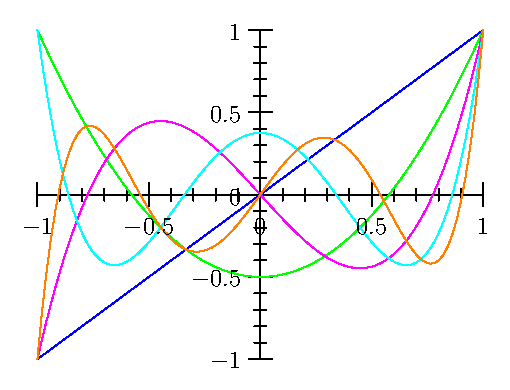
\includegraphics[width=12cm]{figure20.eps}
\caption{Legendre Polynomials}
\label{figure-legendre-polynomials}
\end{figure}

We can notice a number of interesting properties. First, all
the even $P_k$ are even functions, all the odd are odd. The
even one all pass through $(-1,1)$ and $(1,1)$. All the odd
ones pass through $(-1,-1)$ and $(1,1)$. We usually only work
with the Legendre polynomials on the domain $[-1,1]$. We can
notice interesting patterns in the coefficients. We have
powers of $2$ in the denominators, but some are skipped. 
Interesting patterns are also found in the prime divisors of
the numerators.

Here's a list of further interesting properties.
\begin{align*}
P_k(-t) & = (-1)^k P_k(t) \\
\int_{-1}^1 P_k(t) P_l(t) & = \frac{2}{2l+1} \delta_{kl} \\
(k+1)P_{k+1}(t) - (2k+1)tP_k(t) + k P_{k-1}(t) & = 0 \\
(2k+1) P_k(t) & = \frac{d}{dt} \left( P_{k+1}(t) - P_{k-1}(t)
\right) \\
P_k(t) & = \sum_{j=0}^k (-1)^j \binom{k}{j}^2 \left(
\frac{1+t}{2} \right)^{k-j} \left( \frac{1-t}{2} \right)^j
\end{align*}
The $\delta_{kl}$ in the second property is the Kronecker
delta. It evalutes to $1$ if $k=l$ and to $0$ otherwise.
It's a very useful piece of notation. This second property is
an orthogonality property: if we define an inner product of
two functions as the integral of their product over $[-1,1]$,
then the Legendre polynomials are all orthogonal to each
other. In linear algebra language, they form an orthogonal
basis for the infinite dimensional linear space of polynomials
(with this particular inner product). Orthogonal bases are
nice to work with, another fact that recommends the
Legendre polynomials.

The third property is called the functional equation. This
section is the start of a whole branch of mathematicals on
so-called `special functions'. The existence of a functional
equation which relates members of the family to each other is
quite typical for special functions. 

As an interesting aside, let's very briefly detour to talk
about generating functions.

\begin{defn}
If $\{a_n\}_{n=1}^\infty$ is a sequence of real numbers, a
generating function for the sequence is a Taylor series (or
other series in some contexts) where the $a_n$ are the series
coefficients. 
\end{defn}

In some way, the generating function `knows' the properties of
the sequence. I will share two interesting examples. 

\begin{example}
In some way, the function on the left relates to and accounts
for this sequences of integer squares. 
\begin{equation*}
\frac{t(t+1)}{(1-t)^3} = \sum_{n=0}^\infty n^2 t^n
\hspace{1cm} |t| < 1 
\end{equation*}
\end{example}

\begin{example}
This is the generativing function for squares with factorial
denominators.
\begin{equation*}
t(t+1)e^t = \sum_{n=0}^\infty \frac{n^2}{n!} t^n \hspace{1cm}
t \in \RR
\end{equation*}
\end{example}

It turns out, if we briefly allow ourselves to consider
functions of two variables, that there are generating functions for
Legendre polynomials. This relevant identity is
\begin{equation*}
\frac{1}{\sqrt{1- 2tx+x^2}} = \sum_{k=0}^\infty P_k(t) x^n.
\end{equation*}
Somehome, this strange two-variables square root functions
`knows' all the Legendre polynomials. There are all there,
encoded in the Taylor series coefficients.

\section{Issues and Next Directions}
\label{issues}

After these initial examples, two of questions seem
natural. First, we might observe that $P$ and $Q$ were, so
far, only rational functions, which means that we only need to
deal with polynomials in the calculation. What if $P$ and $Q$
were other analytic functions? In this cases, we would have
to expand $P$ and $Q$ as series about the ordinary point and
then multiply them by the series for $y$ in the calculation.
This is possible, but miserable.

We might also wonder why we restricted to homogeneous cases.
What happens if we add a forcing term $f(t)$? We can
certainly do this if $f$ is analytic on the same domain as $P$
and $Q$. In all our examples so far, we compared the
coefficients to $0$. If we have a forcing terms, we would
instead compare the coefficients to the coefficient of $f$
instead of $0$. This leads to more complications, since the
relationship between the coefficients may no longer be a
linear recurrence relation.

In both of these situations (non-polynomial $P$ and $Q$ or
non-homogeneous DE with forcing), we can easily end up in a
situation were the challenges of computation prevent us from
finding a nice form for the coefficients of $y$. Quite
frequently, we will only decide to calculate the first few
terms. The result is a Taylor polynomial approximation to the
solution, instead of a complete Taylor series solution.
However, approximate solutions (if they have sufficient
precision) are often sufficient.

\section{Regular Singular Points}
\label{regular-singular-points}

Throughout this section, we are considering this second order
linear homogeneous differential equation.
\begin{equation*}
y^{\prime \prime} + P(t) y^\prime + Q(t) y = 0
\end{equation*}
Recall that this differential equation has a regular
point if $P(t)$ and $Q(t)$ are analytic at that point. We've
dealt with solutions at ordinary points; now we will consider
solutions at singular points. There are particular types of
singular points which are reasonable to deal with, since the
functions $P$ and $Q$ are quite close to being analytic. Here
is the definition:

\begin{defn}
A singular point $t_0$ of this DE is called a \emph{regular
singular point} if the two functions $(t-t_0)P(t)$ and
$(t-t_0)^2 Q(t)$ are analytic at $t-0$. Equivalently,
$t_0$ is a regular singular point if the limits of $(t-t_0) P(t)$ and
$(t-t_0)^2 Q(t)$ as $t \rightarrow t_0$ exist and are finite. 
(In complex variables terminology, $P(t)$ and $Q(t)$ have
to have poles, not essential singaularities, the pole of $P$
has to be order 1, and the pole of $Q$ has to be order 1 or 2.)
Note that $P$ and $Q$ don't have to be rational
functions for this definition. 
\end{defn}

\subsection{Examples of Regular Singular Points}
\label{examples-rsp}

\begin{example}
\begin{equation*}
y^{\prime \prime} + \frac{y^\prime}{t^3(t-1)^2(t-2)(t-3)(t-4)} +
\frac{y}{t^2 (t-1)(t-2)^2 (t-3)^2 (t-4)^3} = 0 
\end{equation*}
All points other than $t=0,1,2,3,4$ are ordinary points.
Of the singular points, only $t=2,3$ are regular singular
points. The singular points $t=0,1$ have $P(t)$ with a pole of
order 2 or higher (a square term or worse in the denominator),
which is not allowed. The singular point $t=4$ has $Q(t)$
with a pole of order 3 (a cubic term in the denominator),
which is also not allowed.
\end{example}

\begin{example}
\begin{equation*}
y^{\prime \prime} + \cot t y^\prime + y = 0 
\end{equation*}
We use a limit to find the singular points.
\begin{equation*}
\lim_{t \rightarrow 0} t \cot t = \lim_{t \rightarrow 0} \frac{
t \cos t}{\sin t} = 1
\end{equation*}
The limit shows that $t \cot t$ is analytic at $t=0$, so
$t=0$ is a regular singular point.
\end{example}

\subsection{The Method of Frobenius}
\label{frobenius}

The method of Frobenius is a method of constructing solutions
at regular singular points. It relies on this existence
theorem. 

\begin{thm}
Consider a second order homogeneous linear differential
equation.
\begin{equation*}
y^{\prime \prime} + P(t) y^\prime + Q(t) = 0.
\end{equation*}
If $t_0$ is a regular singular point of this equation, then 
there exists at least one (but possibly two) $r \in \RR$ such that
we have a series solution of this form (with $c_0 \neq 0)$).
\begin{equation*}
y = (t-t_0)^r \sum_{n=0}^\infty c_n (t-t_0)^n
\end{equation*}
\end{thm}

This is an extension of the idea of analytic solutions. This
solution is analytic if $r \in \NN$. Otherwise, it is very
close, only differing by this multiple $(t-t_0)^r$. If $r$ is
any negative real number, we have an asymptote at $t=t_0$, so
we can't evaluate there. However, we expect convergence on $0
< |t-t_0| < R$.  If $r$ is a negative integer, we have a new
name for these series.

\begin{defn}
A \emph{Laurent series} is a series of the form
\begin{equation*}
\sum_{n=-\infty}^\infty c_n (t-t_0)^n
\end{equation*}
where $c_n \in \RR$. This is exactly the form of a Taylor
series, but we now allow negative exponents. 
\end{defn}

Now that we have this theorem, and the form of the solution,
we proceed as usual: we throw the form into the differential
equation and see what happens. We expect to have a similar
process for finding the coefficient $c_n$ of the series.
However, we also need a process for finding the number $r$.
Let's assume, for convenience in this derivation, that $t_0 =
0$ is the regular singular point. 

We know that $tP(t)$ and $t^2 Q(t)$ are analytic, from the
definition of a regular singular point. This means that
$P(t)$ and $Q(t)$ can be written in the form
\begin{equation*}
P(t) = \frac{p_{-1}}{t} + \sum_{n=0}^\infty p_n t^n
\hspace{2cm}
Q(t) = \frac{q_{-2}}{t^2} + \frac{q_{-1}}{t} +
\sum_{n=0}^\infty q_n t^n.
\end{equation*}
We will call these Laurent forms for $P$ and $Q$. The
coefficients $p_1$ and $q_2$ will be useful a bit later, so
here are two useful identities to calculate $p_1$ and $q_2$.
\begin{equation*}
p_{-1} = \lim_{t \rightarrow 0 } t P(t) \hspace{2cm}
q_{-2} = \lim_{t \rightarrow 0 } t^2 Q(t) \hspace{2cm}
\end{equation*}
Now we start the method of Frobenious by calculating the
derivatives of $y$ in this new series form.
\begin{align*}
y & = t^r \sum_{n=0}^\infty c_n t^n = \sum_{n=0}^\infty c_n
t^{n+r} \\
y^\prime & = \sum_{n=0}^\infty c_n (n+r) t^{n+r-1} \\
y^{\prime \prime} & = \sum_{n=0}^\infty c_n (n+r) (n+r-1) t^{n+r-2} \\
\end{align*}
(Notice that we don't necessarily lose terms when taking
derivatives; if $r$
is not an integer, there are no constant terms in the series
which go to zero under differentiation. If $r$ is an integer,
we should make a note to worry about derivatives setting
constant terms to zero.)

With these expressions for $y$, $P$ and $Q$, we put it all
together into the original DE.
\begin{align*}
\sum_{n=0}^\infty c_n (n+r) (n+r-1) t^{n+r-2} 
+ P(t) \sum_{n=0}^\infty c_n (n+r) t^{n+r-1} 
+ Q(t) \sum_{n=0}^\infty c_n t^{n+r} & = 0 \\
\sum_{n=0}^\infty c_n (n+r) (n+r-1) t^{n+r-2} 
+ \left(\frac{p_{-1}}{t} + \sum_{n=0}^\infty p_n t^n \right) 
\sum_{n=0}^\infty c_n (n+r) t^{n+r-1} & \\
+ \left( \frac{q_{-2}}{t^2} + \frac{q_{-1}}{t} +
\sum_{n=0}^\infty q_n t^n \right) 
\sum_{n=0}^\infty c_n t^{n+r} & = 0 \\
\end{align*}
This is quite a mess: we have $r$ to determine as well as the
series coefficients. However, we can focus on the coefficient
of the leading term ($t^{r-2}$).
\begin{align*}
r(r-1) c_0 t^{r-2} + \frac{p_{-1}}{t} r c_0 t^{r-1} +
\frac{q_{-2}}{t^2} c_0 t^r & = 0 \\
(r(r-1) + p_{-1} r + q_{-2}) c_0 t^{r-2} & = 0 \\
r(r-1) + p_{-1}r + q_{-2} & = 0 \hspace{1cm} \text{using the
fact that } c_0 \neq 0
\end{align*}

\begin{defn}
This quadratic determines $r$. It is called
the \emph{indicial equation}. 
\end{defn}

So, before we proceed to find the recurrence relations and the
series coefficients, we use this equation to determine $r$.
After finding $r$, the method looks very similar to solutions
at ordinary points. If there are two real roots of the
indicial equation, is seems we'll have to repeat the same
process for each root.  However, in practice, we can leave
$r$ undetermined for most of the procees.

\subsection{Examples}
\label{frobenius-examples}

\begin{example}
\begin{align*}
3ty^{\prime \prime} + y^\prime - y & = 0 \\
P & = \frac{1}{3t} \\
Q & = \frac{-1}{3t} \\
tP & = \frac{1}{3} \implies p_{-1} = \frac{1}{3} \\
t^2 Q & = \frac{-t}{3} \implies q_{-2} = 0 \\
r(r-1) + \frac{r}{3} & = 0 \\
3r^2 - 2r = 0 \implies r & = 0 \text{ or } r = \frac{2}{3} 
\end{align*}
We'll deal with the $r=0$ case first. (Note that $r=0$ means we
get a conventional Taylor series solution.)
\begin{align*}
3t \sum_{n=2}^\infty c_n (n) (n-1) t^{n-2} 
+ \sum_{n=1}^\infty c_n (n) t^{n-1} 
- \sum_{n=0}^\infty c_n t^{n} & = 0 \\
\sum_{n=2}^\infty 3c_n (n) (n-1) t^{n-1} 
+ \sum_{n=1}^\infty c_n (n) t^{n-1} 
- \sum_{n=0}^\infty c_n t^{n} & = 0 \\
\sum_{n=1}^\infty 3c_{n+1} (n+1) n t^n 
+ \sum_{n=1}^\infty c_{n+1} (n+1) t^n 
- \sum_{n=0}^\infty c_n t^{n} & = 0 \\
c_1 - c_0 + \sum_{n=1}^\infty \left[ 3(n+1)n c_{n+1} + (n+1)
c_{n+1} - c_n \right] t^n & = 0 \\
c_{n+1} = \frac{c_n}{3(n^2+n) + n+1} = \frac{c_n}{3n^2 +4n +1}
& = \frac{c_n}{(3n+1)(n+1)} 
\end{align*}
We have the recurrence relation (which is first order this
time), so we start calculating terms.
\begin{align*}
c_0 & = c_0 \\
c_1 & = c_0 \\
c_2 & = \frac{c_1}{(4)(2)} = \frac{c_0}{(4)(2)} \\
c_3 & = \frac{c_2}{(7)(3)} = \frac{c_0}{(7)(4)(3)(2)} \\
c_4 & = \frac{c_3}{(10)(4)} = \frac{c_0}{(10)(7)(4)(4)(3)(2)} \\
c_5 & = \frac{c_4}{(13)(5)} = \frac{c_0}{(13)(10)(7)(4)
(5)(4)(3)(2)} \\
c_n & = \frac{c_0}{n! (4)(7)(10) \ldots (3n-2)} \\
y_1 & = 1 + \sum_{n=1}^\infty \frac{t^n}{n! (4)(7)(10) \ldots
(3n-2)} \\
\end{align*}
This is the solution for $r=0$. Now we proceed to the
$r=\frac{2}{3}$ case. (This is a non-integer exponent, so
the solution is not a conventional Taylor series.)
\begin{align*}
3t \sum_{n=0}^\infty c_n \left(n + \frac{2}{3} \right) \left(n
+ \frac{2}{3}-1 \right)
t^{n + \frac{2}{3}-2} 
+ \sum_{n=0}^\infty c_n \left(n + \frac{2}{3} \right) t^{n + 
\frac{2}{3}-1} - \sum_{n=0}^\infty c_n t^{n + \frac{2}{3}} & =
0 \\ t^{\frac{2}{3}} \left[ \sum_{n=0}^\infty 3c_n \left(n+
\frac{2}{3} \right) \left(n - \frac{1}{3} \right) t^{n-1} 
+ \sum_{n=0}^\infty c_n \left(n+ \frac{2}{3} \right) t^{n-1} 
- \sum_{n=0}^\infty c_n t^{n} \right] & = 0 \\
t^{\frac{2}{3}} \left[ \sum_{n=0}^\infty 3c_n
\left(n + \frac{2}{3} \right) \left( n - \frac{1}{3}
\right) t^{n -1}
+ \sum_{n=0}^\infty c_n \left(n + \frac{2}{3} \right) t^{n-1}
- \sum_{n=1}^\infty c_{n-1} t^{n-1} \right] & = 0 \\
t^{\frac{2}{3}} \left[ \left(3\frac{2}{3} \frac{-1}{3} +
\frac{2}{3} \right) c_0 t^{-1} + \sum_{n=1}^\infty \left[ 3
c_n \left( n+ \frac{2}{3} \right) \left( n - \frac{1}{3}
\right) + c_n \left( n + \frac{2}{3} \right) - c_{n-1} 
\right] t^{n-1} \right] & = 0 \\
\left[ \left( n + \frac{2}{3} \right) \left( 3n - 1 + 1
\right) \right] c_n - c_{n-1} & = 0 \\
c_n = \frac{c_{n-1}}{ \left( n + \frac{2}{3} \right) (3n)} =
\frac{c_{n-1}}{(3n+2)n} & \\
c_{n+1} = \frac{c_n}{(3n+5)(n+1)} & 
\end{align*}
The term in front of $c_0$ reduces to $0$, so $c_0$ is
free. After the first term, we have a recurrence relation, 
so we start calculating terms.
\begin{align*}
c_0 & = c_0 \\
c_1 & = \frac{c_0}{5} \\
c_2 & = \frac{c_1}{(8)(2)} = \frac{c_0}{(8)(5)(2)} \\
c_3 & = \frac{c_2}{(11)(3)} = \frac{c_0}{(5)(8)(11)(2)(3)} \\
c_4 & = \frac{c_3}{(14)(4)} =
\frac{c_0}{(5)(8)(11)(14)(2)(3)(4)} \\
c_5 & = \frac{c_4}{(17)(5)} =
\frac{c_0}{(5)(8)(11)(14)(17)(2)(3)(4)(5)} \\
c_n & = \frac{c_0}{n! (5)(8)(11) \ldots (3n+2)} \\
y_2 & = 1 + \sum_{n=1}^\infty \frac{t^{n + \frac{2}{3}}}{n! (5)(8)
\ldots (3n+2)} \\
y & = A \left( 1 + \sum_{n=1}^\infty \frac{t^n}{n! (4)(7)(10) \ldots
(3n-2)} \right) 
+ B \left( 1 + \sum_{n=1}^\infty \frac{t^{n + \frac{2}{3}}}{n!
(5)(8) \ldots (3n+2)} \right) 
\end{align*}
The radius of convergence here is $R = \infty$, which we can
find by ratio test. It is good to note, though, that there
are no guarantees about the radius of convergence with the
method of Frobenius.

In this example, we could have gone as far as the recurrence
relation using an arbitrary $r$ to avoid repetition. We do
need to specify $r$ once we get to the recurrence relation.
\end{example}

\begin{example}
\begin{equation*}
ty^{\prime \prime} + y = 0 
\end{equation*}
Here $P =0$ and $Q=\frac{1}{t}$, so $p_{-1} = 0$ and $q_{-2} = 0$.
That means the indicial equation is $r(r-1) = 0$ with roots
$r=0$ and $r=1$. We start with the case $r=0$.
\begin{align*}
t \sum_{n=2}^\infty n(n-1)c_n t^{n-2} + \sum_{n=0}^\infty c_n
t^n & = 0 \\
\sum_{n=2}^\infty n(n-1)c_n t^{n-1} + \sum_{n=0}^\infty c_n
t^n & = 0 \\
\sum_{n=1}^\infty (n+1)nc_n t^n + \sum_{n=0}^\infty c_n
t^n & = 0 \\
c_0 + \sum_{n=1}^\infty \left[ (n+1)nc_n + c_n \right] 
t^n & = 0 \\
c_{n+1} & = \frac{-c_n}{(n+1)(n)} \\
c_0 & = 0 \\
c_1 & = c_1 \\
c_2 & = \frac{-c_1}{2} \\
c_3 & = \frac{-c_2}{(3)(2)} = \frac{c_1}{(3)(2)}\\
c_4 & = \frac{-c_3}{(4)(3)} = \frac{-c_1}{(4)(3)(3)(2)(2)} \\
c_5 & = \frac{-c_4}{(5)(4)} = \frac{c_1}{(5)(4)(4)(3)(3)(2)(2)} \\
c_n & = \frac{(-1)^{n+1} c_1}{n! (n-1)!} \\
y_1 & = \sum_{n=1}^\infty \frac{(-1)^{n+1} t^n}{n!(n-1)!}
\end{align*}
Then we calculate with $r=1$. Note the bounds in this case:
since the series doesn't have a constant term, we only loose
one term in the second derivative.
\begin{align*}
t \sum_{n=1}^\infty (n+1)nc_n t^{n-1} + \sum_{n=0}^\infty c_n
t^{n+1} & = 0 \\
\sum_{n=1}^\infty (n+1)nc_n t^n + \sum_{n=0}^\infty c_n
t^{n+1} & = 0 \\
\sum_{n=1}^\infty (n+1)nc_n t^n + \sum_{n=1}^\infty c_{n-1}
t^n+ & = 0 \\
(n+1)n c_n + c_{n-1} & = 0 \\
c_n & = \frac{-c_{n-1}}{(n+1)(n)} \\
c_{n+1} & = \frac{-c_n}{(n+2)(n+1)} \\
c_0 & = c_0 \\
c_1 & = \frac{-c_0}{2} \\
c_2 & = \frac{-c_1}{(3)(2)} = \frac{c_0}{(3)(2)}\\
c_3 & = \frac{-c_2}{(4)(3)} = \frac{-c_0}{(4)(3)(3)(2)(2)} \\
c_4 & = \frac{-c_3}{(5)(4)} = \frac{c_0}{(5)(4)(4)(3)(3)(2)(2)} \\
c_n & = \frac{(-1)^{n} c_0}{(n+1)! n!} \\
y_1 & = \sum_{n=0}^\infty \frac{(-1)^n t^{n+1}}{(n+1)!n!} \\
y_1 & = \sum_{n=1}^\infty \frac{(-1)^{n+1} t^n}{n!(n-1)!}
\end{align*}
Very curiously, we get the same series. The two roots don't lead to two
independent series, but to the same series. We would need other
information to get the second solutions. In general, finding
another solution can be quite difficult. With the method of
Frobenius, we are not guaranteed to find both solutions.
\end{example}

\subsection{Multiple Solutions in the Method of Frobenius}
\label{frobenius-multiple-solutions}

We have a theorem which deals with the situation in the
previous example, where both roots gave the same series.

\begin{thm}
In the setting of the method of Frobenius, assume that $r_1$
and $r_2$ are two real roots of the indicial equation.
Without loss of generalization, assume that $r_1 \geq r_2$.
Then there are three cases.

\begin{itemize}
\item[Case 1:] If $r_1 - r_2 \notin \NN$ then each root will
derive a linearly independent series solutions. (The idea
here is that different fractional or irrational exponents lead
to radically different behaviour.)
\item[Case 2:] If $r_1 - r_2 \in \NN$ but $r_1 \neq r_2$, then
the second root may not produce a new linearly independent
solution. If it doesn't, and both roots produce the solution
$y_1$, then a second solution exists and has the form:
\begin{equation*}
y_2 = a y_1 \ln t + \sum_{n=0}^\infty b_n t^{n+r_2}.
\end{equation*}
In this case, we would need to do extra work to find the
constant $a$ and the series coefficients $b_n$.
\item[Case 3] If the two roots are the same, then (obviously)
only one series solution is generated. A second solution
exists and has the same form as the previous case.
\end{itemize}
\end{thm}

The proof of this theorem relies on another differential
equation technique called \emph{reduction of order}. I've
chosen not to cover that technique in this courses, but it is
good to be aware that it exists. In general, if we have one
solution to a second order linear DE, then reduction of order
is a method for using that solution to change the second order
DE into a first order DE, which can then be solved by first
order methods.

\begin{thm}[Reduction of Order]
Assume that $y_1$ is a solution of homogeneous linear second
order DE of the form
\begin{equation*}
y^{\prime \prime} + P(t) y^\prime + Q(t) = 0.
\end{equation*}
Then a second linearly independent is given by the formula
\begin{equation*}
y_2 = y_1(t) \int \frac{e^{- \int P(t) dt}}{y_1^2(t)} dt.
\end{equation*}
This reduction of order technique is fairly impractical for
series solution, since dividing by $y_1^2$ and then
integrating is a miserable calculation. 
\end{thm}

\section{Bessel Functions}
\label{bessel-functions}

\subsection{The $\Gamma$ Function}
\label{gamma-function}

Before we get to a very interesting example of the method of
Frobenious, we need to define the $\Gamma$ (gamma)function.
This is a ubiquitous and useful function which generalizes the
factorial. 

\begin{defn}
The $\Gamma$ function is defined by this integral
\begin{equation*}
\Gamma(t) = \int_0^\infty x^{t-1}e^{-x} dx.
\end{equation*}
The $\Gamma$ function is defined on all $\RR$ except 0 and
negative integers. It is continuous and differentiable on $(0,
\infty)$. 
\end{defn}

There are several important properties of $\Gamma(t)$:
First, (as mentioned) it generalizes the factorial.
\begin{align*}
\Gamma(a+1) & = a \Gamma(a) \\
\Gamma(1) & = 1 \\
\Gamma(n) & = (n-1)! \text{ for } n \in \NN 
\end{align*}
Asymptotically, the factorial nature of the $\Gamma$ functions
means it grows faster than $e^t$. 

If the positive integer values of the $\Gamma$ function
generalize the factorial, what can be expect for other values?
The results are surprising. Look at the value of
$\Gamma(\frac{1}{2})$ (in this calculation, we use a
well-known result for the integral $e^{-u^2}$).
\begin{align*}
\Gamma \left( \frac{1}{2} \right) & = \int_0^\infty
x^{-\frac{1}{2}} e^{-x} dx \\
x & = u^2 \\
dx & = 2u du \\
x^{-\frac{1}{2}} & = \frac{1}{u} \\
& = 2 \int_0^\infty e^{-u^2} u \frac{1}{u} du \\
& = 2 \int_0^\infty e^{-u^2} \\
& = 2 \frac{\sqrt{\pi}}{2} = \sqrt{\pi}
\end{align*}
Then, from the factorial-like nature of $\Gamma$, all
other half-integer values are multiples of $\sqrt{\pi}$.
\begin{equation*}
\Gamma\left( \frac{2n+1}{2} \right) = \frac{ (3)(5)(7) \ldots
(2n-1) \sqrt{\pi}}{2^n} 
\end{equation*}

\subsection{Bessel's Equation}
\label{bessel-equation}

The method of Frobenius is used to solve a historically
interesting equation: Bessel's Equation. This equation shows
up in harmonic problems with certain cirucular boundary
conditions, such as the vibrations on a drum. It is also
useful for springs with fatigue (where the spring constant
gets weaker over time), the quantum model of the hydrogen
atom, and various electical/gravitational potentials
(particular those which are circularly or spherically
symmetric). Its solutions are another piece of the mathematics
of special functions.

Let $\nu \in \RR$. Bessel's equation of order $\nu$ is the
equation
\begin{equation*}
t^2 y^{\prime \prime} + t y^\prime + (t^2 - \nu^2) y = 0.
\end{equation*}
Written in standard form, $0$ is a regular singular point of
Bessel's equation.
\begin{align*}
P(t) & = \frac{1}{t} \implies p_{-1} = 1 \\
Q(t) & = 1-\frac{\nu^2}{t^2} \implies q_{-2} = -\nu^2 \\
\end{align*}
We calculate the indicial equation.
\begin{align*}
r(r-1) + r - \nu^2 & = 0 \\
r^2 -r + r - \nu^2 & = 0 \\
r^2 & = \nu^2 \\
r & = \pm \nu
\end{align*}
We start with $r = \nu$ first and assume that $\nu \geq
0$ without loss of generality. We calculate the derivatives of
$y$.
\begin{align*}
y & = \sum_{n=0}^\infty c_n t^{n+\nu} \\
y^\prime & = \sum_{n=0}^\infty c_n(n+\nu) t^{n+\nu- 1} \\
y^{\prime\prime} & = \sum_{n=0}^\infty c_n(n+\nu)(n+\nu-1)
t^{n+\nu- 2} 
\end{align*}
Then we proceed with a lengthly calculation.
\begin{align*}
t^2 y^{\prime \prime} + t y^\prime + (t^2 - \nu^2) y & = 0 \\
t^2 \sum_{n=0}^\infty c_n(n+\nu)(n+\nu-1)
+ t \sum_{n=0}^\infty c_n(n+\nu) t^{n+\nu- 1} 
+ t^2 \sum_{n=0}^\infty c_n t^{n+\nu} 
- \nu^2 \sum_{n=0}^\infty c_n t^{n+\nu} & = 0 \\
\sum_{n=0}^\infty c_n(n+\nu)(n+\nu-1) t^{n+\nu} 
+ \sum_{n=0}^\infty c_n(n+\nu) t^{n+\nu} 
+ \sum_{n=0}^\infty c_n t^{n+\nu+2} 
- \sum_{n=0}^\infty \nu^2 c_n t^{n+\nu} & = 0 \\
\sum_{n=0}^\infty c_n(n+\nu)(n+\nu-1) t^{n+\nu} 
+ \sum_{n=0}^\infty c_n(n+\nu) t^{n+\nu} 
+ \sum_{n=2}^\infty c_{n-2} t^{n+\nu} 
- \sum_{n=0}^\infty \nu^2 c_n t^{n+\nu} & = 0 \\
\nu(\nu-1) c_0 t^\nu + (\nu+1) \nu c_1 t^{\nu+1} + \nu c_0 t^\nu
+ (\nu+1)c_1t^{\nu+1} - \nu^2 c_0 t^\nu - \nu^2 c_1 t^{\nu+1} & \\
+ \sum_{n=2}^\infty c_n(n+\nu)(n+\nu-1) t^{n+\nu} 
+ \sum_{n=2}^\infty c_n(n+\nu) t^{n+\nu} 
+ \sum_{n=2}^\infty c_{n-2} t^{n+\nu} 
- \sum_{n=2}^\infty \nu^2 c_n t^{n+\nu} & = 0 \\
\nu(\nu-1) c_0 t^\nu + (\nu+1) \nu c_1 t^{\nu+1} + \nu c_0 t^\nu
+ (\nu+1)c_1t^{\nu+1} - \nu^2 c_0 t^\nu - \nu^2 c_1 t^{\nu+1} & \\
+ \sum_{n=2}^\infty \left[ c_n(n+\nu)(n+\nu-1) 
+ c_n(n+\nu) + c_{n-2} - \nu^2 c_n \right] t^{n+\nu} & = 0 
\end{align*}
Look at the coefficient of $t^{\nu}$.
\begin{align*}
\left( (\nu^2 - \nu) c_0 +\nu c_0 - \nu^2 c_0 \right) & = 0 \\
\left( \nu^2 - \nu + \nu - \nu^2 \right) c_0 & = 0 \\
0 c_0 & = 0 
\end{align*}
Therefore, $c_0$ is free. Look at the coefficient of
$t^{\nu+1}$.
\begin{align*}
\left( \nu(\nu+1)c_1 + (\nu+1) c_1 - \nu^2 c_1 \right) & = 0 \\
\left( \nu^2 + \nu + \nu + 1 - \nu^2 \right) c_1 & = 0 \\
\left( 2 \nu + 1 \right) c_1 & =0 \\
\end{align*}
So $c_1 = 0$ unless $\nu = \frac{-1}{2}$. However, we assumed
that we were dealing with $\nu$ positive, so we conclude that
$c_1 = 0$. (We'll pay some special attention to $\nu =
\frac{-1}{2}$ when we look at negative $\nu$, and to
half-integer values of $\nu$ in general.)

Then we have the general recurrence relation, for $n \geq 2$.
\begin{align*}
((n+\nu)(n+\nu-1) + n + \nu - \nu^2) c_n + c_{n-2} & = 0 \\
(n^2 + n\nu + n\nu + \nu^2 - n - \nu + n + \nu - \nu^2 ) c_n &
= -c_{n-2} \\
(n^2 + 2n\nu) c_n & = -c_{n-2} \\
c_n & = \frac{-c_{n-2}}{n(n+2\nu)} \\
c_{n+2} & = \frac{-c_n}{(n+2)(n+2+2\nu)} 
\end{align*}
These are the equations that calculate coefficients, so we
start calculating. 
\begin{align*}
c_0 & = c_0 \\
(2\nu+1) c_1 & = 0 \implies c_1 = 0 \implies c_{2n+1} = 0 \
\forall n \in \NN \\
c_2 & = \frac{-c_0}{2(2+2\nu)} \\
c_4 & = \frac{c_0}{(2)(4)(2+2\nu)(4+2\nu)} \\
c_6 & = \frac{-c_0}{(2)(4)(6)(2+2\nu)(4+2\nu)(6+2\nu)} \\
c_8 & = \frac{c_0}{(2)(4)(6)(8)(2+2\nu)(4+2\nu)(6+2\nu)
(8+2\nu)} \\
c_{2n} & = \frac{(-1)^n c_0}{2^{2n} n! (1+\nu)(2+\nu) \ldots
(n+\nu)}
\end{align*}
The constant $c_0$ is still undetermined. By convention, the
choice for $c_0$ is this strange value
\begin{equation*}
c_0 = \frac{1}{2^\nu \Gamma(1+\nu)}.
\end{equation*}
The properties of the $\Gamma$ function allow us to simplify the
denominator of the $c_n$.
\begin{equation*}
c_{2n} = \frac{(-1)^n}{2^\nu \Gamma(1+\nu)} \frac{1}{2^{2n}n!
(\nu+1) \ldots (\nu+n)} = \frac{(-1)^n}{2^{2n+v} n!
\Gamma(1+n+\nu)} 
\end{equation*}
With this simplification, we can write the final solution for
positive $\nu$. 

\begin{defn}
The solution constructed above is written $J_\nu$ and called
the Bessel function of the first kind of order $\nu$.
\begin{equation*}
J_{\nu} = \sum_{n=0}^\infty \frac{(-1)^n}{n! \Gamma(1+n+\nu)}
\left( \frac{t}{2} \right)^{2n+\nu} 
\end{equation*}
It converges on $(0, \infty)$. It may not be defined at 0 or
negative numbers. In general, we are only interested in the
Bessel function on the domain $(0, \infty)$. The Bessel
functions of the first kind for $\nu \in \ZZ$ are show in
Figure \ref{figure-bessel-first-kind}.
\end{defn}

\begin{figure}[t]
\centering
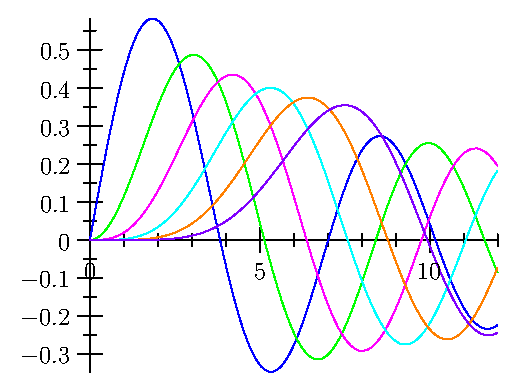
\includegraphics[width=11cm]{figure21.eps}
\caption{Integer-Order Bessel Functions of the First Kind}
\label{figure-bessel-first-kind}
\end{figure}

\begin{figure}[t]
\centering
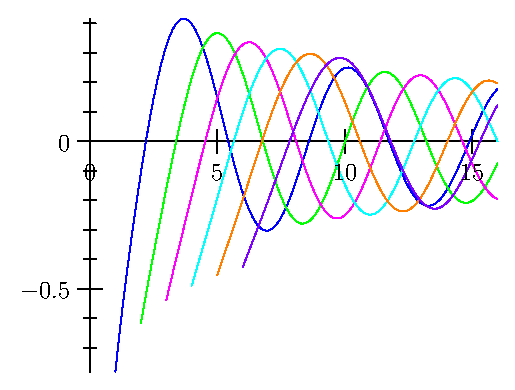
\includegraphics[width=11cm]{figure22.eps}
\caption{Integer-Order Bessel Functions of the Second Kind}
\label{figure-bessel-second-kind}
\end{figure}

We could redo the same work for negative $\nu$, but it is
very similar (for $n = \frac{-1}{2}$, we would get a term
$(2\nu - 1) c_1$, so we would still conclude that $c_1 = 0$,
hence all odd coefficients are $0$). In this way, we find the
rest of the Bessel functions of the first kind.
\begin{equation*}
J_{-\nu} = \sum_{n=0}^\infty \frac{(-1)^n}{n! \Gamma(1+n-\nu)}
\left( \frac{t}{2} \right)^{2n-\nu} 
\end{equation*}
One caution should be noted. If $n \in \NN$, this $J_{-n}$
gives an undefined denominator, hence doesn't define a series. 
In these cases, the method of Frobenius gives $J_{-n} =
(-1)^n J_{n}$. This is not necessarily surprising: in the
method of Frobenius, is the roots of the indicial equation
differ by an integer, we may not have linearly independent
solution. If $\nu \notin \ZZ$, then we have
two linearly independent solutions, as we would
expect with the method of Frobenius.

\begin{defn}
Let $n \notin \ZZ$. The \emph{Bessel function of the second
kind} of order $\nu$ are written $Y_{\nu}$ and defined by this
expression
\begin{equation*}
Y_{\nu} = \frac{\cos (\nu \pi) J_{\nu}(t) - J_{-\nu}(t)}{\sin \nu
\pi}.
\end{equation*}
This definition is a linear combination of Bessel functions of
the first kind. For $\nu \in \ZZ$, this linear combination
have been just a multiple of the one solution we know. To get
around this, for $\nu \in \ZZ$, we define the Bessel function
of the second kind as a limit.  
\begin{equation*}
Y_{\nu}(t) = \lim_{\alpha \rightarrow \nu} Y_{\alpha}(t)
\end{equation*}
L'Hopital's rule shows that this limit exists.  The Bessel
functions of the second kind are shown in Figure
\ref{figure-bessel-second-kind}. 
\end{defn}

To summarize, for any $\nu \geq 0$ we have $J_{\nu}$ and
$Y_{\nu}$, two linearly independent solutions to the
differential equation. The general solution is
\begin{equation*}
y = A J_{\nu} + B Y_{\nu}.
\end{equation*}

\subsection{The Aging Spring}
\label{aging-spring}

Consider the spring equation from before.
\begin{equation*}
my^{\prime \prime} + by^\prime + ky = 0
\end{equation*}
Now, instead of all constants, lets assume this is an
aging spring. That is, at time passes, the spring constant
decreases. One model is exponential decay, so let $k(t) = ke^{-\alpha
t}$ for $\alpha > 0$. Let's see what happens without friction.
\begin{equation*}
m y^{\prime \prime} + ke^{-\alpha t} = 0 
\end{equation*}
Here's a strange change of variables.
\begin{align*}
s & = \frac{2}{\alpha} \sqrt{\frac{k}{m}} e^{\frac{-\alpha t}{2}} \\
\frac{ds}{dt} & = \frac{2}{\alpha} \frac{-\alpha}{2} \sqrt{
\frac{4k}{m\alpha^2}} e^{\frac{-\alpha t}{2}} = -
\sqrt{\frac{k}{m}} e^{-\frac{\alpha t}{2}} \\
\frac{d^2s}{dt^2} & = \frac{\alpha}{2} \sqrt{\frac{k}{m}}
e^{-\frac{\alpha t}{2}} \\
\frac{dy}{dt} & = \frac{dy}{ds} \frac{ds}{dt} \\
\frac{d^2 y}{dt^2} & = \frac{d}{dt} \left( \frac{dy}{ds}
\frac{ds}{dt} \right) \\
& = \frac{d^2 s}{dt^2} \frac{dy}{ds} + \frac{ds}{dt}
\frac{d}{dt} \frac{dy}{ds} \\
& = \frac{d^2 s}{dt^2} \frac{dy}{ds} + \frac{ds}{dt}
\frac{d^2y}{ds^2} \frac{ds}{dt} \\
& = \frac{d^2 s}{dt^2} \frac{dy}{ds} + \left( \frac{ds}{dt}
\right)^2 \frac{d^2 y}{ds^2} \\
& = \frac{\alpha}{2} \sqrt{\frac{k}{m}} e^{-\frac{\alpha
t}{2}} \frac{dy}{ds} + \frac{k}{m} e^{-\alpha t} \frac{d^2
y}{ds^2}
\end{align*}
All this nonsense allows us to alter the original
equation as follows. (The change from the third to the fourth
line involves dividing by $m$, then dividing by $\alpha^2$,
then multiplying by 4.)
\begin{align*}
m y^{\prime \prime} + ke^{-\alpha t} & = 0 \\
m \left(\frac{d^2 s}{dt^2} \frac{dy}{ds} + \left( \frac{ds}{dt}
\right)^2 \frac{d^2 y}{ds^2} \right) + ke^{-\alpha t} & = 0 \\
\frac{m\alpha}{2} \sqrt{\frac{k}{m}} e^{-\frac{\alpha t}{2}}
\frac{dy}{ds} + m \frac{k}{m} e^{-\alpha t} + k e^{-\alpha t} y
& = 0 \\
\frac{2}{\alpha} \sqrt{\frac{k}{m}} e^{-\frac{\alpha t}{2}}
\frac{dy}{ds} + \frac{4}{\alpha^2} \frac{k}{m} e^{-\alpha t}
\frac{d^y}{ds^2} + \frac{4k}{m\alpha^2} e^{-\alpha t} y & = 0 \\
s^2 \frac{d^2y}{ds^2} + s \frac{dy}{ds} + s^2 y & = 0 
\end{align*}
This is Bessel's equation with $\nu = 0$. It is
solved by Bessel's functions (of the first and second kind)
for $\nu = 0$.
\begin{align*}
y & = A J_0(s) + B Y_0(s) \\
& = A J_0 \left( \frac{2}{\alpha} \sqrt{\frac{k}{m}}
e^{-\frac{\alpha t}{2}} \right) + B Y_0 \left( \frac{2}{\alpha}
\sqrt{\frac{k}{m}} e^{-\frac{\alpha t}{2}} \right) 
\end{align*}
These functions completely describe the behaviour of an aging
spring with exponential decay of the spring constant.

\subsection{Properties of the Bessel Functions}
\label{bessel-functions-properties}

We have some nice symmetry properties for integer orders. Let
$m \in \ZZ$. 
\begin{align*}
J_{-m}(t) & = (-1)^m J_m(t) \\
J_m(-t) & = (-1)^m J_m(t) 
\end{align*}
We mentioned a functional equation for the Legendre
polynomials. We have one here as well; this one is true for
arbitrary $\nu$.
\begin{equation*}
tJ_{\nu}^\prime(t) = \nu J_{\nu}(t) - t J_{\nu+1}(t) 
\end{equation*}
There are some interesting properties of Bessel functions with
half-integer orders. Look closely again at $J_{\frac{1}{2}}$. 
\begin{align*}
J_{\frac{1}{2}}(t) & = \sum_{n=0}^\infty \frac{(-1)^n}{n!
\Gamma(\frac{3}{2} + n))} \left( \frac{t}{2} \right)^{2n +
\frac{1}{2}} \\
\Gamma \left( \frac{3}{2} + n \right) & =
\frac{(2n+1)!}{2^{2n+1} n!} \sqrt{\pi} \\
J_{\frac{1}{2}}(t) & = \sum_{n=0}^\infty \frac{(-1)^n}
{\frac{(2n+1)!}{2^{2n+1}n!} \sqrt{\pi}} \left( \frac{t}{2}
\right)^{2n + \frac{1}{2}} \\
& = \sqrt{\frac{2}{\pi t}} \sum_{n=0}^\infty
\frac{(-1)^n}{(2n+1)!} t^{2n+1} \\
& = \sqrt{\frac{2}{\pi t}} \sin t \\
J_{-\frac{1}{2}} & = \sqrt{\frac{2}{\pi t}} \cos t
\end{align*}
These special half-integer function can actually be expressed
as elementary functions. The decay of the amplitude of these
waves is $\frac{1}{\sqrt{t}}$ not $e^{-t}$; this decay is
much slower than exponential decay. The half-integer Bessel
functions are called \emph{spherical Bessel functions}. The
reason for that name is that they solve the wave equation in
spherical coordinates. The wave equation in $\RR^3$ is
$\nabla^2 A + k^2 A = 0$ for $\nabla^2$ the Laplacian.
Changing to spherical coordinates and restricting to the
radial terms gives Bessel's equation with half-integer order.

We can think of these half-integer Bessel functions as the
standing waves of spherical harmonic systems.
$J_{\frac{1}{2}}$ is the first harmoinc, then
we get higher harmonics as we go. The typical image of these
spherical waves are the decaying amplitude ripples radiating
from a stone dropped in a pond.

\chapter{Laplace Transforms}
\label{laplace-transforms}

\section{Definitions}
\label{laplace-transforms-definitions}

In functional analysis, we have a group of operations on
functions called transforms. These operations act on a
certain set of functions and transform then into new functions:
through the transforms, we see behaviour that was previously
hidden.

The changes due to transforms are often radical: the resulting
functions do not look anything like the originals. We can
think of transforms as radically altering the environment of
the function, so that everything changes into a surprisingly
different form.

For those who like to think in linear algebra terms, we can
think of the space of functions defined on some interval in $\RR$
as a vector space. (The specific vector space depends on the
interval and the class of function: continuous,
piecewise-continuous, differentiable, etc). In this language,
transforms are nothing but interesting linear transformations
between vector spaces of functions.

In this section, we study the Laplace transform. It applies to
a functions with certain controls on their asymptotic growth,
which we now define.  

\begin{defn}
A function $f(t)$ defined on $[0,
\infty)$ is of \emph{exponential order c} if $\exists M > 0 \ \
\exists T > 0$ such that $\forall t > T \ \ \ |f(t)| <
Me^{ct}$. Asymptotically, this is equivalent to $f \in
\calO(e^{ct})$ for some real positive $c$. 
\end{defn}

If $f(t)$ is a piecewise-continuous function on $[0, \infty)$
of exponential order $c$, then its Laplace transform is 
\begin{equation*}
\calL \{ f(t) \} (s) = \int_0^\infty e^{-st} f(t) dt.
\end{equation*}
The Laplace transform is defined on the domain $(c, \infty)$.
We can check that this improper integral converges
for all $s \in (c, \infty)$. 

The restriction of exponential order is a fairly reasonable
one: in differential equations and applied mathematics, we
are rarely concerned with functions which grow faster
than the exponential. 

The choice of variables is standard for Lapalce transforms.
We will often refer to the original functions as functions in
the $t$-domain, and to their transforms as functions in the
$s$-domain. In addition, if $f(t)$ and $g(t)$ are function in
the $t$-domain, we will also often write $F(s)$ and $G(s)$ for
their Laplace transforms. By convention, we use lower case for
the $t$-domain and uppercase for the matching function in
the $s$-domain.

Most of the following examples are sub-exponential, so we expect
a transform on $(0, \infty)$. Note that we are never guaranteed
convergence at $0$. 

\begin{example}
\begin{align*}
\calL \{ 1 \} & = \int_0^\infty e^{-st} dt = \left.
\frac{-e^{-st}}{s} \right|_0^\infty = \lim_{a \rightarrow \infty}
\frac{-e^{-sa} + 1}{s} = \frac{1}{s} \\
\calL \{ t \} & = \int_0^\infty te^{-st} dt = \lim_{a
\rightarrow \infty} \left[ \left. \frac{-te^{-st}}{s}
\right|_0^a + \int_0^a \frac{e^{-st}}{s} dt \right] \\
& = \lim_{a \rightarrow \infty} \left[ \frac{0 - ae^{-sa}}{s} +
\left. \frac{-e^{-st}}{s^2} \right|_0^a \right] = \frac{1}{s^2}
\\
\calL \{ t^n \} & = \int_0^\infty t^ne^{-st} dt =
\frac{n!}{s^{n+1}} \\
\calL \{ e^{at} \} & = \int_0^\infty e^{-st}e^{at} dt =
\int_0^\infty e^{at-st} dt = \left. \frac{e^{at-st}}{a-s}
\right|_0^\infty = \frac{-1}{a-s} = \frac{1}{s-a} \hspace{2cm}
s \in (a, \infty)
\end{align*}
Our first observation about Laplace transforms is simply their
strangeness. Powers of $t$ turn into inverse powers of $s$,
but exponentials (which are very different) turn into very
similar reciprocals.
\end{example}

\begin{example}
We said that Lapalce transforms exist for piecewise-continuous
functions with a certain exponential order. Here is an
example for a piecewise continuous function and its transform.
\begin{align*}
f(t) & = \left\{ \begin{matrix} 0 & t \in [0,1] \\ t & t \in [1,
\infty) \end{matrix} \right. \\
\calL \{ f(t) \} & = \int_0^\infty f(t) e^{-st} dt \\
& = \int_1^\infty te{-st} dt = \left. \frac{-te^{-st}}{s}
\right|_1^\infty + \int_1^\infty \frac{e^{-st}}{s} dt \\
& = \frac{-e^{-s}}{s} + 0 + \left. \frac{-e^{-st}}{s^2}
\right|_1^\infty = \frac{-e^{-s}}{s} - \frac{e^{-s}}{s^2} =
\frac{-(s+1)e^{-s}}{s^2} 
\end{align*} 
The Laplace transform is not a piecewise function, even
thought the original was. 
\end{example}

\begin{example}
The Laplace transform of $t^n$ for $n \in \ZZ$ involved
factorials, so it is not surprising that $t^\alpha$ for
non-integer $\alpha$ involves the extension of the factorial:
the $\Gamma$ function.
\begin{align*}
\calL \{ t^\alpha \} & = \int_0^\infty e^{-st} t^{\alpha} dt \\
& = \int_0^\infty t^{(\alpha + a) - 1} e^{-st} \\
u & = st \\
& = \int_0^\infty \left( \frac{u}{s} \right)^{(\alpha+1)-1}
e^{-u} \frac{du}{s} \\
& = \frac{1}{s^{\alpha +1}} \int_0^\infty u^{(\alpha+ 1)-1}
e^{-u} du = \frac{\Gamma(\alpha +1)}{s^{\alpha +1}}
\end{align*} 
\end{example}

\begin{example}
Finally, Laplace transforms are defined for some important
oscillating functions, such as the trigonometric functions and
the Bessel functions. 
\begin{align*}
\calL \{ \sin t \} & = \int_0^\infty e^{-st} \sin t dt = \frac{1}{s^2+1} \\
\calL \{ \cos t \} & = \frac{s}{s^2+1} \\
\calL \{ J_0(kt) \} & = \frac{1}{\sqrt{s^2 + k^2}}
\end{align*} 
Again, note the strangeness: even starting with transcendental
and non-elementary functions like these, the Lapalce
transforms are rational and algebraic functions.
\end{example}

As an aside, I mentioned at the start of this chapter that the
Laplace transform is not the only transform in mathematics.
The most well-known and well-used transform is the 
Fourier transform. It uses the same conventions about the $s$
and the $t$ domains, but it applies to complex valued
functions. In place of the $e^{-st}$ term in the Laplace
transform, the Fourier transform uses the complex $e^{-2\pi
\imath st}$. 

\begin{defn}
The \emph{Fourier transform} of a function $f(s)$ is given by
this integral.
\begin{equation*}
\hat{f}(s) = \int_{-\infty}^\infty f(t) e^{-2\pi \imath t s} dt 
\end{equation*}
\end{defn}

\section{Properties of the Laplace Transform}
\label{laplace-transforms-properties}

\subsection{First Properties}
\label{first-properties}

\begin{prop}
The Laplace transform (like all reasonable operations
in analysis) is linear.
\begin{align*}
\calL \{ f+ g \} & = \calL \{ f \} + \calL \{ g \} \\
\calL \{ c f(t)\} & = c \calL \{ f \} 
\end{align*} 
\end{prop}

As we will discover, the Laplace transform is not
multiplicative. The question of how we deal with products
($\calL \{ fg \}$) will come later.

Second, the asymptotic order of $f$ was important to allowing
the definition of the Laplace transform. However, all the
transforms we've seen so far are decaying functions. This is a
general statment: for any function $f(t)$ of exponential order
$c > 0$, we have
\begin{equation*}
\lim_{s \rightarrow \infty} \calL \{ f(t) \} (s) = 0.
\end{equation*}
This property is a useful check: if you ever get a Laplace
transform which doesn't have this limit, you've made a
mistake.

For the same students who like linear algebra, this gives us a
specific understanding of the Laplace transform.  Let
$EOF(0,\infty)$ be the space of piecewise-continuous functions
of exponential order defined on $(0, \infty)$ ($EOF$ for
exponential order functions). Let $DF^+$ be the set of
continuous functions which are defined on $(a, \infty)$ for
some $a > 0$ and have limit $0$ as $s \rightarrow \infty$ (DF
for decay functions). These are both linear spaces, since
addition, subtraction and multiplication by constants preserve
the properties of definition. The the Laplace transform is a
linear map
\begin{equation*}
\calL : EOF(0,\infty) \rightarrow DF^+.
\end{equation*}

\subsection{Shifts}
\label{shifts}

We said we'd return to Laplace transforms of products. We
still can't handle the general case, but there is a nice
property for multiplication by an exponential function.

\begin{prop}
\begin{align*}
\calL \{ e^{at} f(t) \} (s) & = \int_0^\infty e^{at} f(t)
e^{-st} dt \\
& = \int_0^\infty f(t) e^{at-st} dt = \int_0^\infty f(t)
e^{(a-s)t} dt \\
& = \calL \{ f(t) \} (s-a)
\end{align*} 
Multiplication by $e^{at}$ in the $t$ domain results in a 
shift by $a$ in the $s$ domain. This also adjust the domain
of $s$, reflected the fact that multiplication by $e^{at}$
adjusts the exponential order.
\end{prop}

Shifts are quite important in the whole theory. We can also
ask what happens when we shift in the $t$ domain. 

\begin{defn}
The \emph{unit step function} $u_a(t)$ if defined as
\begin{equation*}
u_a(t) = \left\{ \begin{matrix} 0 & t < a \\ 1 & t \geq a.
\end{matrix} \right. 
\end{equation*}
\end{defn}

The unit step function $u_a(t) f(t)$ cancels any part of $f$
for $t<a$, but preserves $f$ for $t \geq a$. To define a shift
of $f$, we can write $u_a(t) f(t-a)$ to remove anything before
$t=0$ from $f$. (Note that we're allowed piecewise continuous
function for Laplace transforms.) We calculate to find the
result of this shift in the $t$-domain.
\begin{align*}
\calL \{ u_a(t) \} (s) & = \int_0^\infty u_a(t) e^{-st} dt =
\int_a^\infty e^{-st} dt \\
 & = \left. \frac{-e^{-st}}{s} \right|_a^\infty =
\frac{e^{-as}}{s} \\
\calL \{ u_a (t) f(t-a)\} (s) & = \int_a^\infty e^{-st} f(t-a) dt
\\
v & = t-a \\
& = \int_0^\infty e^{-s(v+a)} f(v) dv = e^{-sa} \int_0^\infty
e^{-sv} f(v) dv \\
& = e^{-sa} \calL \{ f(t) \} (s) = e^{-sa} F(s)
\end{align*} 
There is a nice parallel here, though it's not a perfect
symmetry. Shifts in one domain correspond to
multiplication by exponentials in the other domain.

\section{Distributions}
\label{distributions}

In the world of functional analysis and the use of transforms,
it turns out we can extend our notion of a function in strange
and novel ways. While I'm not going to give a formal
definition, these extensions are called distributions. The
basic idea is that a distribution may not be a well-defined
function, but it is something that behaves well in
integration. (If the word `distribution' reminds you of
probability and statistics, that's a good intuition. These
distributions are very similar to distributions used in
statistics).

The distribution we will be using in this section is the
$\delta$-function. (The name is terrible, since it is most
certainly \emph{not} a function.) 

\begin{defn}
The $\delta$-function is a distribution with values
\begin{equation*}
\delta_a(t) = \left\{ \begin{matrix} \infty & t = a \\ 0 & t
\neq a \end{matrix} \right.
\end{equation*}
This is not a function, since $\infty$ is not a valid
output for a function. However, this does give us an intuition.
We can think of $\delta_a(t)$ as a thing which is zero away
from $t=a$ and has an infinitely tall spike at $t=a$. Often,
this is defined by a limit. 
\end{defn}

Let $b > 0$ and consider the bell curve function
$\frac{\sqrt{b}}{\sqrt{\pi}} e^{-b(t-a)^2}$. All of these
functions have integral $1$, by design of the choice of the
coefficient.
\begin{equation*}
\int_{-\infty}^\infty \frac{\sqrt{b}}{\sqrt{\pi}} e^{-b(t-a)^2} dt =
\frac{\sqrt{b}}{\sqrt{\pi}} \int_{-\infty}^\infty e^{-b(t-a)^2} dt =
\frac{\sqrt{b}}{\sqrt{\pi}} \frac{ \sqrt{\pi}}{\sqrt{b}} = 1
\end{equation*}

\begin{figure}[t]
\centering
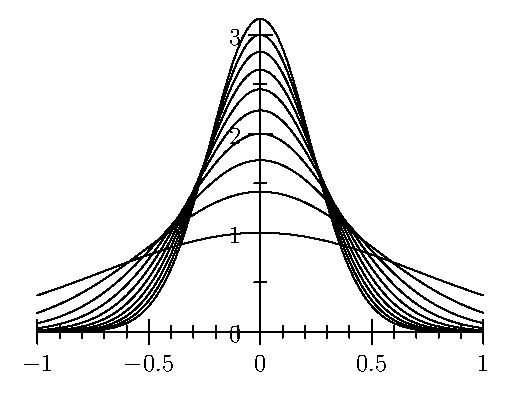
\includegraphics[width=11cm]{figure23.eps}
\caption{Narrower and Narrower Bell Curves}
\label{figure-bell-curves}
\end{figure}

These functions are all bell curves, but they become taller
and narrower at $b$ increases. Figure \ref{figure-bell-curves} shows
the progression of these bell curves.

Then we could define $\delta_a(t)$ as 
\begin{equation*}
\delta_a(t) = \lim_{b \rightarrow \infty}
\frac{\sqrt{b}}{\sqrt{\pi}} e^{b(t-a)^2}.
\end{equation*}
The delta function is the limit of these functions. The
intuition before, of an infinitely narrow and infinitely tall
spike, fits this limit process, since the bell curves are
becoming taller and narrower with each step.  The value of the
integral is unchanged for the entire limit process.
Since integration works well with limits, the integral of the
delta function should be 1.
\begin{equation*}
\int_{-\infty}^\infty \delta_a(t) dt = 1
\end{equation*}
We said that distribution worked well with integration and we
just defined the integral of $\delta_a$ over $\RR$. Now
we can think about integrating products $f(t) \delta_a(t)$.

If we integrate $f(t) \frac{\sqrt{a}}{\sqrt{\pi}} e^{-at^2}$,
we get a weighted average of $f(t)$ values near $a$. In the
limit, though, only the value at $f(a)$ matters, since we
multiply by zero everywhere else. This gives the most
convenient proprety of $\delta$-function.
\begin{equation*}
\int_{-\infty}^\infty \delta_a (t) f(t) dt = f(a)
\end{equation*}
In some sense, the $\delta$-functions are the nicest possible
functions to integrate, since their integrals are just
evaluations of functions. 

Since the $\delta$-function, and distributions in general,
work well with integration, we can take their Laplace
transforms. The Laplace transform for the $\delta$-function
is very easy to calculate.
\begin{equation*}
\calL \{ \delta_a(t) \} (s) = \int_0^\infty \delta_a (t) e^{-st}
dt = \left\{ \begin{matrix} 
0 & a < 0 \\ 
1 & a = 0 \\ 
e^{-as} & a \geq 0 
\end{matrix} \right.
\end{equation*}
Again, this is quite an odd result. We started with a
distribution which wasn't even a proper function, but it's
Laplace transform is a proper, well-behaved differentiable
function.  

Before we end this section, we can ask why we would define
such a strange function. Let's think about harmonic systems
and forcing terms again. The $\delta$-function can act as a
forcing term; if it does, it represents an instantaneous jolt
to the system. The standard image of a harmonic system is a
mass on a spring. In this image, a $\delta$-function
represents hitting the mass with a hammer at one moment in
time. The force only acts for an instant, but it transfers
some finite energy and causes a change in the system.

\section{Laplace Transforms and Derivatives}
\label{derivatives}

This is a course on differential equations; if Laplace
transforms are useful, we will need them to relate to
derivatives. Let's calculate what happens to a derivative of
a function (of exponential order) in a Laplace transform.
\begin{align*}
\calL \left\{ \frac{df}{dt} \right\} & = \int_0^\infty
\frac{df}{dt} e^{-st} dt \\
& = \left. fe^{-st} \right|_0^\infty - \int_0^\infty (-s) f(t)
e^{-st} dt \\
& = \lim_{a \rightarrow \infty} f(a) e^{-sa} - f(0) + s \calL \{
f(t) \} (s) = -f(0) + s F(s)
\end{align*} 
We can sumarize the result in a rule.
\begin{equation*}
\calL \{ f^\prime(t) \} (s) = -f(0) + sF(s).
\end{equation*}
This is a lovely and convenient property. In the $s$-domain,
there is no more differentiation. We just have multiplication
by the $s$ term and evaluation of the function at a point. 

We can do a similar calculation for second derivatives. The
calculation will involve two uses of integration by parts,
though we can make use of the previous calcullation to
simplify the work.
\begin{align*}
\calL \left\{ \frac{d^2f}{dt^2} \right\} & = \int_0^\infty
\frac{d^2f}{dt^2} e^{-st} dt \\
& = \left. \frac{df}{dt} e^{-st} \right|_0^\infty +
s\int_0^\infty \frac{df}{dt} e^{-st} dt \\
& = -f^\prime(0) - sf(0) + s^2 F(s)
\end{align*} 
Again, this is very convenient. The derivatives are
completely removed in the $s$-domain, replaced with simple
algebraic operations. The general result for any order of
differentiation is
\begin{equation*}
\calL \left\{ \frac{d^n f}{dt^n} \right\} = s^n F(s) - s^{n-1}
f(0) - s^{n-2} f^\prime(0) - s^{n-3} f^{\prime \prime}(0) -
\ldots - f^{(n-1)}(0).
\end{equation*}
This leads to the amazing use of Laplace transforms in solving
DEs. A Laplace transform change differentiation into simple
algebraic operations; therefore, it should change some DEs
into algebraic equations. Since algebraic equations are much
easier to solve than DEs, this is a huge advantage. However,
we have one problem. If we want to solve a DE, we want to
solve it in the $t$-domain. We can transform to the $s$-domain
and solve the algebraic equation, but we need to get back to
the $t$-domain to finish. For this, we need to invert the
transform, which we will defined in the next section. 

Before we move on, here are two other properties of the Laplace
transform which relate to derivatives. The first shows that
integrals are also changed into something algebraic.
\begin{equation*}
\calL \left\{ \int_0^t f(u) du \right\} = \frac{1}{s} \calL \{
f(t) \} 
\end{equation*}
The second is a parallel identity which shows how
differentiation in the $s$-domain also comes from an algebraic
operation on the $t$-domain.
\begin{equation*}
\calL \{ t^n f(t) \} = (-1)^n \frac{d^n}{ds^n} \calL \{ f(t) \} 
\end{equation*}

\section{Inverse Laplace Transforms}
\label{inverse-transforms}

We would like an operation $\calL^{-1}$ which undoes the
Laplace transform.
\begin{equation*}
\calL^{-1} \left\{ \calL \{ f(t) \} \right\} = f(t) 
\end{equation*}
This is very difficult to calculate directly, and the
construction of the inverse transform is beyond the scope of
this course. (It relies on complex ananlysis.) I'll state the
result for completeness.

\begin{thm}
Let $\alpha$ be a real number which is larger than all
real singularities of $F(s)$. Let $\gamma$ be a path in $\CC$
which goes in a straight line from $\alpha - \imath T$ to
$\alpha + \imath T$. 
\begin{equation*}
\calL^{-1} (F(s)\} = \frac{1}{2\pi \imath} \lim_{T \rightarrow
\infty} \int_{\gamma} e^{st} F(s) ds 
\end{equation*}
\end{thm}

Note this is a contour integral in $\CC$, a common object in
the study of complex variables. The use of the
distance to singularities makes sense in that discipline,
since contour integrals depend on the location of
singularities. For those with a background in complex
variable, note that this is not a closed curve and the
homotopy implications depend a great deal on the function $F$.

For our purposes, we'll just use tables to find inverse
Laplace transforms, using the functions we already know. We'll
try to turn the $s$ domain answers into familiar forms and
invert known functions. This is a bit tricky, but can often be
done. The use of shifts will be particularly inportant. 
We should note that $\calL^{-1}$ is also linear.

We can make a table of the most important inverse transforms.
\begin{align*}
\calL^{-1} \left\{ \frac{n!}{s^{n+1}} \right\} & = t^n \\
\calL^{-1} \left\{ \frac{1}{s-a} \right\} & = e^{at} \\
\calL^{-1} \left\{ \frac{k}{s^2 + k^2} \right\} & = \sin kt \\
\calL^{-1} \left\{ \frac{s}{s^2 + k^2} \right\} & = \cos kt \\
\calL^{-1} \left\{ \frac{k}{s^2 - k^2} \right\} & = \sinh kt \\
\calL^{-1} \left\{ \frac{s}{s^2 -k^2} \right\} & = \cosh kt \\
\calL^{-1} \left\{ e^{-sa} \right\} & = \delta_a(t)
\end{align*} 
The shift in an inverse transform is captured by the rule 
\begin{equation*}
\calL^{-1} \left\{ e^{-sa} F(s) \right\} = u_a(t) f(t-a).
\end{equation*}
This shifts of trigonometric functions are common enough that
it is useful to mention them here.
\begin{align*}
\calL^{-1} \left\{ \frac{\beta}{(s+ \alpha)^2 + \beta^2}
\right\} & = e^{-\alpha t} \sin \beta t \\
\calL^{-1} \left\{ \frac{s + \alpha}{(s+ \alpha)^2 + \beta^2}
\right\} & = e^{-\alpha t} \cos \beta t 
\end{align*}

\section{Using Laplace Transforms to Solve Linear DEs}
\label{laplace-linear-odes}

As we've seen, Laplace transforms turn derivatives into
algebraic operations. Therefore, particularly for certain
linear equations, we can expect Laplace transforms to turn DEs
into algebraic equations. We'll start with a very well known
case: homogeneous second order constant coefficient linear
equations. 

\begin{example}
\begin{equation*}
y^{\prime \prime} + y = 0 \hspace{2cm} y(0) = 1 \hspace{1cm}
y^\prime(0) = 0
\end{equation*}
We apply the Laplace transform, making use of the initial
values when we transform the derivative.
\begin{align*}
\calL \{ y^{\prime \prime} + y \} & = 0 \\
(s^2Y - sy(0) - y^\prime(0)) + Y & = 0 \\
s^2Y - s + Y & = 0 \\
(s^2+1)Y & = s \\
Y & = \frac{s}{s^2 + 1} \\
y & = \calL^{-1} \left\{ \frac{s}{s^2+1} \right\} = \cos t
\end{align*} 
We recover the expected $y(t) = \cos t$, but without any
calculation of the characteristic equation or interpretation
of complex roots. We also didn't have to get the complete
solution and solve for unknown constants, since we made use of
the initial values in the process. If initial values were not
given, we would have to use unknown constants in their place
in the calculation.
\end{example}

\begin{example}
Let's move on to a move involved harmonic system and 
assume that $b^2 - 4mk < 0$, so that we know to expect
sinusoidal solutions. 
\begin{equation*}
my^{\prime \prime} + b y^\prime + ky = 0 \hspace{2cm} y(0) =
1 \hspace{1cm} y^\prime(0) = \frac{-b}{2m}
\end{equation*}
Then we can apply the Laplace transform to the entire equation.
\begin{align*}
\calL \{ my^{\prime \prime} + b y^\prime + ky \} & = \calL \{ 0
\} \\
m (s^2Y - sy(0) - y^\prime(0)) + b(sY - y(0)) + kY & = 0 \\
Y(ms^2 + bs + k) - ms - b + \frac{b}{2} & = 0 \\
Y & = \frac{ms+\frac{b}{2} }{ms^2+bs+k} 
= \frac{s + \frac{b}{2m}}{s^2 + \frac{b}{m} s + \frac{k}{m}} \\
& = \frac{s + \frac{b}{2m}}{ \left( s^2 + \frac{b}{m} s +
\frac{b^2}{4m^2} \right)+ \left( \frac{k}{m} - \frac{b^2}{4m^2}
\right) } \\
& = \frac{s + \frac{b}{2m}}{ \left( s + \frac{b}{2m} \right)^2 +
\left( \frac{4km - b^2}{4m^2} \right)} \\
y & = \calL^{-1} \left\{ \frac{s + \frac{b}{2m}}{ \left( s + \frac{b}{2m}
\right)^2 + \left( \frac{4mk - b^2}{4m^2} \right)} \right\} \\
& = e^{-\frac{b}{2m}t} \cos \left( \frac{\sqrt{4mk-b^2}}{2m} t
\right) 
\end{align*} 
Now let's add a forcing term. Since we can take a Laplace
transform of a delta function, we'll use that for the forcing
term. $F\delta_0(t)$ is a sudden impact with force $F$ (in
appropriate units) at time $t$. We'll use initial values of
$y(0) = y^\prime(0) = 0$, so that the system is initially at
rest. Again, we'll assume that $b^2 -4km < 0$ for harmonic motion. 

\begin{align*}
my^{\prime \prime} + by^\prime + ky & = F \delta_0(t) \\
\calL \{ my^{\prime \prime} + by^\prime + ky \} & = \calL \{ F
\delta_0(t) \} \\ 
m (s^2 Y - s y(0) - y^\prime(0)) + b(sY - y(0)) + kY & = F \\
(ms^2 + bs + k) Y & = F \\
Y & = \frac{F}{ms^2 + bs + k} \\
Y & = \frac{\frac{F}{m}}{s^2 + \frac{b}{m}s + \frac{k}{m}} \\
Y & = \frac{\frac{F}{m}}{\left( s^2 + \frac{bs}{m} +
\frac{b^2}{4m^2} \right) + \left( \frac{k}{m} - \frac{b^2}{4m^2}
\right) } \\
Y & = \frac{F}{m} \frac{2m}{\sqrt{4km-b^2}}
\frac{\frac{\sqrt{4km-b^2}}{2m}}{\left( s + \frac{b}{2m} \right)^2 +
\left( \frac{4km - b^2}{4m^2} \right) } \\
y(t) & = \frac{2m}{4km-b^2} \frac{F}{m} e^{\frac{-b}{2m}t} \sin \left(
\frac{\sqrt{4km-b^2}}{2m}t \right) \\
y(t) & = \frac{2F}{4km-b^2} e^{\frac{-b}{2m}t} \sin \left(
\frac{\sqrt{4km-b^2}}{2m}t \right) \\
\end{align*} 
We could ask: what changes if we move the impact to a later
time? If the impact is at $t=4$, then the forcing term is 
$\delta_4(t)$. We again proceed with the Laplace transform.

\begin{align*}
my^{\prime \prime} + by^\prime + ky & = F \delta_4(t) \\
\calL \{ my^{\prime \prime} + by^\prime + ky \} & = \calL \{ F
\delta_0(t) e^{-4s}\} \\ 
m (s^2 Y - s y(0) - y^\prime(0)) + b(sY - y(0)) + kY & = F
e^{-4s} \\
(ms^2 + bs + k) Y & = F e^{-4s} \\
Y & = \frac{Fe^{-4s}}{ms^2 + bs + k} \\
Y & = \frac{\frac{Fe^{-4s}}{m}}{s^2 + \frac{b}{m}s + \frac{k}{m}} \\
Y & = e^{-4s} \frac{\frac{F}{m}}{\left( s^2 + \frac{bs}{m} +
\frac{b^2}{4m^2} \right) + \left( \frac{k}{m} - \frac{b^2}{4m^2}
\right) } \\
Y & = e^{-4s} \frac{F}{m} \frac{2m}{\sqrt{4km-b^2}}
\frac{\frac{\sqrt{4km-b^2}}{2m}}{\left( s + \frac{b}{2m} \right)^2 +
\left( \frac{4km - b^2}{4m^2} \right) } \\
y(t) & = u_4(t) \frac{2m}{4km-b^2} \frac{F}{m}
e^{\frac{-b}{2m}(t-4)} \sin \left(
\frac{\sqrt{4km-b^2}}{2m} (t-4) \right) \\
y(t) & = u_4(t) \frac{2F}{4km-b^2} e^{\frac{-b}{2m} (t-4) } \sin
\left( \frac{\sqrt{4km-b^2}}{2m} (t-4) \right) \\
\end{align*} 
Unsurprinsingly, we get precisely the same wave, just shifted $4$
units to the right. 
\end{example}

\begin{example}
This example has an exponential forcing term.
\begin{align*}
y^{\prime \prime} + 4y^\prime + 4y & = e^{-2t} \\
y(0) & = 0 \hspace{2cm} y^\prime(0) = 2 \\
s^2 Y - sy(0) - y^\prime(0) + 4(sY - y(0)) + 4Y & = \frac{1}{s+2}
\\
s^2 Y - 2 + 4sY + 4Y & = \frac{1}{s+2} \\
(s^2 + 4s + 4)Y & = \frac{1}{s+1} + 2 = \frac{2s+3}{s+2} \\
Y & = \frac{2s+3}{(s+2)(s+2)^2} = \frac{2s+3}{(s+2)^3} \\
Y & = \frac{2}{(s+2)^2} + \frac{1}{(s+2)^3} \\
y & = 2te^{-2t} + t^2e^{-2t} = e^{-2t}(2t+t^2)
\end{align*} 
\end{example}

\begin{example}
This example has a linear forcing term. 
\begin{align*}
y^{\prime \prime} + 4y & = 4t^2 - 4t + 10 \\
y(0) & = 0 \hspace{2cm} y^\prime(0) = 3 \\
s^2 Y - sy(0) - y^\prime(0) + 4Y & = \calL \{ 4t^2 - 4t + 10 \}
\\
s^2 Y + 4sY -3 & = \frac{8}{s^3} - \frac{4}{s^2} +
\frac{10}{s}\\
Y & = \frac{8-4s+10s^2 + 3s^3}{s^3(s^2+4)} \\
Y & = \frac{2s^2-s+2}{s^3} + \frac{-2s+4}{s^2+4} \\
& = \frac{2}{s} - \frac{1}{s^2} + \frac{2}{s^3} -
\frac{2s}{s^2+4} + \frac{4}{s^2+4} \\
y & = 2 - t + t^2 - 2 \cos 2t + 2 \sin 2t 
\end{align*} 
\end{example}

\begin{example}
Since we can take Laplace transforms of piecewise-continuous
functions, here is an example with a piecewise forcing term. 
\begin{equation*}
f(t) = \left\{ \begin{matrix} 0 & t \leq \pi \\ 3 \cos t & t >
\pi \end{matrix} \right.
\end{equation*}
This represents a sinusoidal forcing term which is turned of
at time $t=\pi$. We calculate the Lapalce transform of this
piecewise function.
\begin{align*}
y^{\prime \prime} + y & = f(t) \hspace{2cm} y(0) = 0
\hspace{1cm} y^\prime(0) = 0 \\
s^2Y + Y & = 3 \calL \{ u_\pi(t) \cos t\} = 3 \calL \{ -u_\pi(t)
\cos (t-\pi) \} \\
& = -3 e^{-\pi s} \frac{s}{s^2+1} \\
(s^2+1)Y & = \frac{-3se^{-\pi s}}{s^2+1} \\
Y & = \frac{-3se^{-\pi s}}{(s^2+1)^2} \\
Y & = -3e^{-\pi s} \frac{s}{(s^2+1)^2} \\
Y & = -3e^{-\pi s} \frac{1}{2} \frac{d}{dt} \frac{-1}{s^2+1} \\
y & = \frac{-3}{2} u_{\pi}(t) (t-\pi) \sin (t-\pi)
\end{align*} 
Notice that the forcing term is discontinuous, representing a
sudden change, but the resulting solution is still continuous.
The force suddenly changes, but the system still responds
continuously.
\end{example}

\section{Laplace Transforms of Periodic Functions}
\label{laplace-periodic}

Laplace transforms cooperate well with periodic functions. We've
already see this for sine and cosine, but it is also true for
arbitrary, even discontinuous periodic functions. 

\begin{example}
This is the square wave. 
\begin{equation*}
f(t) = \left\{ \begin{matrix} 0 & t \in [2n+1, 2n+2] \\1
& 1 \in (2n, 2n+1) \end{matrix} \right.
\end{equation*}
\end{example}

\begin{example}
This is the sawtooth wave. 
\begin{equation*} \
f(t) = \left\{ t-n \hspace{1cm} t \in [n, n+1) \right.
\hspace{1cm} \forall n \in \NN
\end{equation*}
\end{example}

For each of these functions, doing an integration over
$(0,\infty)$ is problematric. Instead, we have a convenient
theorem for Laplace transforms of such waves.

\begin{prop}
If $f(t)$ is periodic with period $T$, and of exponential
order, then 
\begin{equation*}
\calL\{ f(t) \} = \frac{1}{1-e^{-sT}} \int_0^T e^{-st} f(t) dt.
\end{equation*}
\end{prop}

\begin{example}
\label{example-square-wave}
Let $f(t)$ be the square wave, which has period
2. Then we can use $f$ as a forcing term and solve the
following DE with a Laplace transform (we factor $1-e^{-2s}$
as a difference of squares in this calculation).
\begin{align*}
y^\prime + by & = f(t) \\
sY + bY & = \frac{1}{1-e^{-2s}} \int_0^2 f(t) e^{-st} dt \\
& = \frac{1}{1-e^{-2s}} \int_0^1 e^{-st} dt \\
& = \frac{1}{1-e^{-2s}} \left. \frac{e^{-st}}{-s} \right|_0^1 =
\frac{-(e^{-s}-1)}{s(1-e^{-2s})} \\
& = \frac{1}{s(1+e^{-s})} \\
Y & = \frac{1}{s(s+b)(1-(-e^{-s}))}
\end{align*} 
This expression is problematic for an inverse transform.
Specficially, the $\frac{1}{1-e^{-s}}$ term is the problem. We
solve the problem by expressing it as a geometric series.
\begin{align*}
Y & = \frac{1}{s(s+b)(1-(-e^{-s})} \\
& = \frac{1}{s(s+b)} \left( 1 - e^{-s} + e^{-2s} - e^{-3s} +
\ldots \right) \\
& = \frac{1}{b} \left( \frac{1}{s} - \frac{1}{s +
b}\right) \left( 1 - e^{-s} + e^{-2s} - e^{-3s} +
\ldots \right) \\
& = \frac{1}{b} \left( \frac{1}{s} - \frac{e^{-s}}{s} +
\frac{e^{-2s}}{s} - \frac{e^{-3s}}{s} + \ldots \right) \\
& \hspace{1cm} - \frac{1}{b} \left( \frac{1}{s + b} -
\frac{e^{-s}}{s + b} + \frac{e^{-2}}{s + b}
- \frac{e^{-3}}{s + b} + \ldots \right) \\
y & = \frac{1}{b} \left( 1 - u_1(t) + u_2(t) - u_3(t) + \ldots)
\right) \\
& \hspace{1cm} - \frac{1}{b} \left( e^{-bt} - u_1(t)
e^{-b(t-1)} + u_2(t) e^{-b(t-2)} - u_3(t)
e^{-b(t-3)} + \ldots \right) \\
y & = \frac{1}{b} \left( 1-e^{-bt} \right) + \frac{1}{b}
\sum_{n=1}^\infty (-1)^n u_n(t) (1-e^{-b(t-n)}) 
\end{align*} 
We might ask about convergence, since this is an infinite
series (though not a taylor series, since its terms are
exponentials). We'll leave the technical details of
convergence for now, and trust that the solution of the DE is
attainable and converges for some reasonable domain.
\end{example}

\section{Algebraic Properties of the Laplace Transform}
\label{laplace-algebraic}

We know that the Laplace transform is linear, but we said we
would return to the issue of product. To start, it is easier
to think in reverse: if we have a product $FG$ in the
$s$-domain, where did it come from in the $t$-domain?
Here is the relevant calculation (the change in the order of
integration near the end is jutified by theorems in
multivariable analysis).

\begin{align*}
FG & = \int_0^\infty e^{-st} f(t) df \int_0^\infty e^{-su} g(t)
du \\
& = \int_0^\infty \int_0^\infty e^{-s(u+t)} f(t)g(u) dt du \\
& = \int_0^\infty f(t) \left[ \int_0^\infty e^{-s(u+t)} g(u) du
\right] du \\
v & = u+ t \\
& = \int_0^\infty f(t) \left[ \int_t^\infty e^{-sv} g(v-t) dv
\right) dt \\
& = \int_0^\infty e^{-sv} \left[\int_0^t f(t) g(v-t) dt \right]
dv \\
& = \calL \left\{ \int_0^t f(t) g(v-t) dt \right\} 
\end{align*} 
The product $FG$ in the $s$-domain turns into this strange
integral-based combination of the function $f$ and $g$. This
is a new `product'; it is called a convolution.

\begin{defn}
Let $f,g$ be integrable function on $[0,\infty)$. Their
convoluiton is defined by this integral.
\begin{equation*}
f \star g (t) = \int_0^t f(\tau) g(t-\tau) d \tau.
\end{equation*}
\end{defn}

The convolution takes two functions and produces a new
function, so it is a product. However, it is a strange product
with new properties. 

\begin{prop}
\begin{smallitemize}
\item The convolution is commutative: $f \star g = g \star f$. 
\item The convolution is associative: $(f \star g) \star h = f
\star (g \star h)$. 
\item The convolution is distributive: $f \star (g \pm h) = f
\star g \pm f \star h$. 
\item The convolution respect constants. $a (f \star g) = (af)
\star g = f \star (ag)$
\item The Laplace transform turns convolutions into products:
\begin{equation*}
\calL \left\{ f \star g \right\} = F(s) G(s)
\end{equation*}
\end{smallitemize}
\end{prop}

Here is an interesting question: if this is a product, what is the
identity? That is, what function $g$ satisfies
\begin{equation*}
f \star g = \int_0^t f(\tau) g(t-\tau) d \tau = f(t).
\end{equation*}
In this question, the integral needs to evaluate $f(\tau)$
at $\tau = t$. We know a `function' that does this:
$\delta_0$. 
\begin{equation*}
f \star \delta_0 = \int_0^t f(\tau) \delta_0 (t-\tau) d \tau =
f(t) 
\end{equation*}

\begin{prop}
The $\delta$-function at 0 is the identity for the convolution. 
\end{prop}

The convolution behaves well with differentiation.
\begin{equation*}
\frac{d}{dt} (f \star g) = \frac{df}{dt} \star g = g \star
\frac{dg}{dt} \\
\end{equation*}
It also behaves well with integration.
\begin{equation*}
\int_0^\infty f \star g dt = \int_0^\infty f(t) dt \int_0^\infty
g(t) dt 
\end{equation*}
Finally, it lets us understand inverse Lapalce transforms of
products.
\begin{align*}
\calL^{-t} \left\{ \frac{k^2}{(s^2+k^2)^2} \right\} & = \calL^{-1}
\left\{ \frac{k}{s^2+k^2} \frac{k}{s^2+k^2} \right\} \\
& = \sin kt \star \sin kt \\
& = \int_0^t \sin ku \sin (kt-ku) du \\
& \text{Using } \left[ \sin A \sin B = \frac{1}{2} \cos (A-B) - \cos (A+B) \right] \\
\calL^{-t} \left\{ \frac{k^2}{(s^2+k^2)^2} \right\} 
& = \frac{1}{2} \int_0^t \cos (ku - kt + ku) - \cos (ku + kt -
ku ) du \\
& = \frac{1}{2} \int_0^t \cos (2ku - 2t) - \cos (kt) du \\
& = \frac{1}{2} \left. \frac{\sin (2ku - kt)}{2k} \right|_0^t -
\left. \frac{1}{2} u \cos (kt) \right|_0^t \\
& = \frac{\sin (2kt-kt) - \sin (-kt)}{4k} - \frac{t\cos kt}{2}
\\
& = \frac{\sin (kt)}{2k} - \frac{t\cos kt}{2} = \frac{\sin kt -
kt \cos kt}{2k} 
\end{align*} 
In addition to differential equations, sometimes we get
integral equations in mathematics. Laplace transforms and
convolutions can help solve certain types of integral
equations.

\begin{align*} 
3t^2 - e^{-t} - \int_0^t f(u) e^{t-u} du & = f(t) \\
3t^2 - e^{-t} - f \star e^t & = f(t) \\
\frac{6}{s^3} - \frac{1}{s+1} - F(s) \frac{1}{s-1} & = F(s) \\
\frac{6}{s^3} - \frac{1}{s+1} & = F(s) \left( 1 + \frac{1}{s+1}
\right) \\
\frac{6}{s^3} - \frac{1}{s+1} & = F(s) \left( \frac{s}{s-1}
\right) \\
F(s) & = \frac{6(s-1)}{s^4} - \frac{(s-1)}{s(s+1)} \\
& = \frac{6}{s^3} - \frac{6}{s^4} + \frac{1}{s} - \frac{2}{s+1}
\\
f & = 3t^2 - t^3 + 1 - 2e^{-t} \\
\end{align*}

\section{More Examples of Solving DEs with Laplace
Transforms}
\label{laplace-examples}

\begin{example}
Consider a slightly different version of the square wave.
\begin{equation*}
f(t) = \left\{ \begin{matrix} 1 & t \in [2n, 2n+1) \\
-1 & t \in [2n+1, 2n+2) \end{matrix} \right.
\end{equation*}
Using initial conditions $y(0) = y^\prime(0)= 0$ we solve the
equation $y^{\prime \prime} + y = f(t)$. 
\begin{align*}
(s^2+1)Y & = \frac{1}{1-e^{-2s}} \int_0^2 e^{-st} f(t) dt \\
& = \frac{1}{1-e^{-2s}} \left[ \int_0^1 e^{-st} dt - \int_1^2
e^{-st} dt \right] \\
& = \frac{1}{1-e^{-2s}} \left[ \left. \frac{e^{-st}}{-s}
\right|_0^1 + \left. \frac{e^{-st}}{s} \right|_1^2 \right] \\
& = \frac{1}{1-e^{2s}} \left[ \frac{-e^{-s}}{s} + \frac{1}{s} +
\frac{e^{-2s}}{s} - \frac{e^{-s}}{s} \right] \\
& = \frac{1-2s^{-s} + e^{-2s}}{s(s^2+1)} \frac{1}{1-e^{-2s}} \\
& = \frac{1}{s(s^2+1)} (1-2e^{-s} + e^{-2s}) ( 1 - e^{-2s} +
e^{-4s} - e^{-6s} + e^{-8s} - \ldots ) \\
& = \left( \frac{-s}{s+1} + \frac{1}{s} \right) (1 - 2e^{-s} +
2e^{-3s} - 2e^{-5s} + 2e^{-7s} - \ldots )
\\
y & = 1 - \cos t - 2u_1(t) (1-\cos(t-1)) + 2u_3(t) (1-\cos(t-3))
\\
& \hspace{1cm} - 2u_5 (t) (1-\cos(t-5)) + 2 u_7(t) (1 - \cos
(t-7) ) - \ldots \\
& = 1 - \cos t + 2\sum_{k=0}^\infty (-1)^{k+1} u_{2k+1} (t) (1 -
\cos(t-(2k+1)))
\end{align*}
As with the previous square wave solution in Example
\ref{example-square-wave}, this solution
involves an infinite series of shifts, each one slightly
further along. Periodic functions always lead to an infinite
series of shifts.
\end{example}

\begin{example}
This examples also involves a step function.
\begin{align*}
y^{\prime \prime} + 6y^\prime + 5y & = t - tu_2(t) \hspace{1cm}
y(0) = 1 \hspace{1cm} y^\prime(0) = 0 \\
s^2 Y - s + 6sY - 6 + 5Y & = \frac{1}{s^2} - e^{-2s} \left(
\frac{1}{s^2} - \frac{2}{s} \right) \\
(s+5)(s+1) Y & = \frac{1}{s^2} - \frac{e^{-2s}}{s^2} +
\frac{2e^{-2s}}{s} + s + 6 \\
Y & = \frac{1}{s^2(s+1)(s+5)} - \frac{e^{-2s}}{s^2(s+1)(s+5)} +
\frac{2e^{-2s}}{s(s+1)(s+5)} \\
& \hspace{1cm} + \frac{s}{(s+5)(s+1)} +
\frac{6}{(s+5)(s+1)} \\
& = \frac{1}{5s^2} + \frac{1}{4(s+1)} - \frac{1}{100(s+5)} -
\frac{6}{25s} - \frac{e^{-2s}}{5s^2} - \frac{e^{-2s}}{4(s+1)} +
\frac{e^{-2s}}{100(s+5)} \\
& \hspace{1cm} + \frac{6e^{-2s}}{25s} -
\frac{e^{-2s}}{2(s+1)} + \frac{e^{-2s}}{10(s+5)} +
\frac{2e^{-2s}}{5s} + \frac{5}{4(s+5)} - \frac{1}{4(s+1)} \\
& \hspace{1cm} - \frac{3}{2(s+1)} + \frac{3}{2(s+5)} \\
Y & = \frac{1}{5s^2} - \frac{6}{25s} + \frac{3}{20(s+1)} +
\left( \frac{-1}{100} + \frac{5}{4} + \frac{3}{2} \right)
\frac{1}{s+5} \\
& \hspace{1cm} + e^{-2s} \left( \frac{1}{5s^2} + \left(
\frac{6}{25} + \frac{2}{5} \right) \frac{1}{s} + \left(
\frac{-1}{4} - \frac{1}{2} \right) \frac{1}{s+1} +
\left(\frac{1}{100} + \frac{1}{10} \right) \frac{1}{s+5} \right)
\\
& = \frac{1}{5s^2} - \frac{6}{25s} - \frac{3}{2(s+1)} +
\frac{137}{50(s+5)} \\
& \hspace{1cm} + e^{-2s} \left( \frac{1}{5s^2} +
\frac{16}{25s} - \frac{3}{4(s+1)} + \frac{11}{100(s+5)} \right) \\
y & = \frac{t}{5} - \frac{6}{25} - \frac{3e^{-t}}{2} +
\frac{137e^{-5t}}{50} + u_2(t) \left[ \frac{(t-2)}{5} +
\frac{16}{25} - \frac{3e^{2-t}}{4} + \frac{11e^{10-5t}}{100}
\right] \\
y & = \frac{t}{5} - \frac{6}{25} - \frac{3e^{-t}}{2} +
\frac{137e^{-5t}}{50} + u_2(t) \left[ \frac{t}{5} +
\frac{6}{25} - \frac{3e^{2-t}}{4} + \frac{11e^{10-5t}}{100}
\right] 
\end{align*}
\end{example}

\begin{example}
This example uses two $\delta$-functions, representing
two sudden impacts.
\begin{align*}
y^{\prime \prime} - 7y^\prime + 6y & = e^t + \delta_2(t) +
\delta_4(t) \hspace{1cm} y(0) = y^\prime(0) = 0 \\
s^2 Y - 7sY + 6Y & = \frac{1}{s-1} + e^{-2s} + e^{-4s} \\
Y & = \frac{1}{(s-1)(s-6)(s-1)} + \frac{e^{-2s}}{(s-6)(s-1)} +
\frac{e^{-4s}}{(s-6)(s-1)} \\
& = \frac{-1}{25(s-1)} - \frac{1}{5(s-1)^2} + \frac{1}{25(s-6)}
\\
& \hspace{1cm} + e^{-2t} \left( \frac{1}{5(s-6)} -
\frac{1}{5(s-1)} \right) \\
& \hspace{1cm} + e^{-4t} \left( \frac{1}{5(s-6)} -
\frac{1}{5(s-1)} \right) \\
y & = \frac{e^{-t}}{25} - \frac{1}{2} \calL^{-1} \left\{
\frac{d}{dt} \frac{-1}{s-1} \right\} + \frac{1}{25} e^{6t} \\
& \hspace{1cm} \frac{u_2(t)}{5} \left( e^{6(t-2)}- e^{t-2}
\right) + \frac{u_4(t)}{5} \left( e^{6(t-4)}- e^{t-4} \right) \\
y & = \frac{e^{-t}}{25} - \frac{te^t}{5} + \frac{1}{25} e^{6t} \\
& \hspace{1cm} \frac{u_2(t)}{5} \left( e^{6t-12}- e^{t-2} \right) +
\frac{u_4(t)}{5} \left( e^{6t-24}- e^{t-4} \right) 
\end{align*} 
\end{example}

\begin{example}
This is a ridiculous example with infinitely many
$\delta$-functions, representing a new impact at every unit of
time.
\begin{align*}
f(t) & = \sum_{n=0}^\infty \delta_n (t) \\
y^{\prime \prime} + 3 y^\prime + 2y & = f(t) \hspace{1cm} y(0) =
y^\prime(0) = 0 \\
s^2 Y + 3sY + 2Y & = \frac{1}{1-e^{-s}} \int_0^1 e{-st} \delta_0
(t) dt = \frac{1}{1-e^{-s}} \\
Y & = \frac{1}{1-e^{-s}} \frac{1}{(s+2)(s+1)} \\
Y & = \left( \frac{1}{s+1} - \frac{1}{s+2} \right) \left( 1 _
e^{-s} + e^{-2s} + e^{-3s} + e^{-4s} + \ldots \right) \\
y & = e^{-t} - e^{-2t} 
+ u_1(t) \left( e^{-(t-1)} - e^{-(2t-2)} \right) 
+ u_2(t) \left( e^{-(t-2)} - e^{-(2t-4)} \right) \\
& \hspace{1cm} + u_3(t) \left( e^{-(t-3)} - e^{-(2t-6)} \right) 
+ u_4(t) \left( e^{-(t-4)} - e^{-(2t-8)} \right) \\
y & = e^{-t} - e^{-2t} 
+ u_1(t) \left( e^{1-t} - e^{2-2t} \right) 
+ u_2(t) \left( e^{2-t} - e^{4-2t} \right) \\
& \hspace{1cm} + u_3(t) \left( e^{3-t} - e^{6-2t} \right) 
+ u_4(t) \left( e^{4-t} - e^{8-2t} \right) \\
& = \sum_{k=0}^\infty u_k(t) \left( e^{k-t} - e^{2(k-t)}
\right)
\end{align*}
This is an interesting superposition of decay functions. They
all have the same shape with a slightly higher peak. Adding
them all up gives something which slowly rises higher and
higher, while still trying to decay. Eventually the system
does grow beyond any bounds, even with all the decay
functions.
\end{example}

\begin{example}
This is an example with an integral.
\begin{align*}
\frac{dy}{dt} + 6y(t) + 9 \int_0^t y(u) du & = -1 \hspace{1cm} y(0)
= 0 \\
sY+ 6Y + 9 \frac{Y}{s} & = \frac{-1}{s} \\
s^2 + 6sY + 9Y & = -1 \\
Y & = \frac{-1}{(s+3)^2} = \frac{d}{ds} \frac{1}{s+3} \\
y & = te^{-3t}
\end{align*}
We could try the previous example another way, by first
differentiating both sides.
\begin{align*}
\frac{dy}{dt} + 6y(t) + 9 \int_0^t y(u) du & = -1 \hspace{1cm} y(0)
= 0 \\
\frac{d^2y}{dt^2} + 6 \frac{dy}{dt} + 9y & = 0 \\
r^2 + 6r + 9 & = 0 \implies r = 3 \\
y & = ae^{-3t} + bte^{-3t} \\
y(0) & = 0 \implies a=0 \\
y & = bte^{-3t}
\end{align*}
\end{example}

In this previous example, we would ask: what about $b$? In the
original method, to match with the $-1$, we need $b=1$.
In th second method, since we differentiated both sides of the
equation, we lost the information that determined the constant
$b$.

\chapter{Systems of Differential Equations}
\label{systems}

So far, our differential equations involves one 
dependent variable and one independent variable (typically
time). It's very common to have two or more variables which
all depend on the same independent variable and whose
derivatives interact with each other. This interaction
produces systems of differential equations involving those
functions and their derivatives. This chapter introduces
qualitative analysis of systems of DEs and solutions to linear
systems using Laplace transforms.

\section{Key Examples}
\label{systems-key-examples}

There are a number of important motiavting examples. We first
look to biology, where the interaction of species produces
systems of linear equations. The Lokta-Volterra equations 
model predator-prey relationships. Let $p(t)$ be
the population of prey and $q(t)$ be the population of
predators. These equations describe the
interactions between the two derivatives.
\begin{align*}
\frac{dp}{dt} & = ap - bpq \\
\frac{dq}{dt} & = cpq - dq
\end{align*}
The coefficients $a,b,c$ and $d$ are all positive
coefficients. $a$ is a natural birth rate for the prey, $b$
is the death of prey due to predation, $c$ is the growth rate
of predators due to predation, and $d$ is the natural death
rate of predators. The product $pq$ represents the number of
interactions between predators and prey. The Lokta-Volterra
system is a classic system in mathematical biology;
however, its non-linearity makes it difficult to solve and the
solutions are not expressible by elementary functions. To help
understanding the system without having to actually calculate
difficult solutions, we will develop qualitative methods of
analysis.

Mathematical biology has many systems similar to
Lokta-Volterra. If $p$ and $q$ are two species competing for
the same resources, we have a similar two-equation DE model.
\begin{align*}
\frac{dp}{dt} & = a_pp\left(1- \frac{p + b_p q}{c_p} \right) \\
\frac{dq}{dt} & = a_qp\left(1- \frac{q + b_q p}{c_q} \right)
\end{align*}
The coefficients $a_p$ and $a_q$ are the natural growth rates
of each species, $c_p$ and $c_q$ are the carrying capacities of
the environment for each species, and $b_p$ and $b_q$
measure the effects of competition. 

Infection disease models are also systems of differential
equations. The SIR model is a good example. In a population
exposed to an infection disease, let $S$ be the susceptible
population, $I$ the infected population, and $R$ the recovered
population. The model is this system of three
differential equations.
\begin{align*}
\frac{dS}{dt} & = -a I S \\
\frac{dI}{dt} & = a I S - b I \\
\frac{dR}{dt} & = b I 
\end{align*}
Here $a$ measures the increase in infection due to interactions
between the infected and susceptible population and $b$
measure the natural recovery of the infected population. Many
similar models exist to model infection disease.

Mathematical biology only gets more complex and involved from
here. The following link shows the system of DEs in the 2004
Molecular Biology of the Cell Paper ``Integrative Analysis of
Cell Cycle Control in Budding Yeast'' by K.C. Chen et. al.

\url{http://www.ncbi.nlm.nih.gov/pmc/articles/PMC491841/table/tbl1/}

Examples exist in other disciplines as well. If we go back to
physics, we can look at the physics of the coupled spring. In
this sytem, we have a mass $m_1$ on a spring with spring
constant $k_1$ attached to a fixed object. Then we have a
second mass $m_2$ attached to the first by a spring with
spring constant $k_2$. Analyzing the forces and using Newton's law
of motion results in a system of DEs.
\begin{align*}
m_1x_1^{\prime \prime} & = - k_1x_1 + k_2(x_2 - x_1) \\
m_2x_2^{\prime \prime} & = -k_2(x_2-x_1) 
\end{align*}

\section{Qualitative Methods}
\label{systems-qualitative-methods}

For first order autonomous equations, we used a phase-line
analysis to determine the steady states and the trajectories
of movement between the steady states. We analyzed the
stability of the steady states, and the phase line gave a
fairly complete picture of the behaviour of the system
depending on an initial value. For systems of DEs, the same
analysis applies; however, for each function involved in the
system, we get an additional dimension of analysis. In this
section, for ease of drawing the analysis, we restrict to
systems with two functions and two equations.

Let's write $p(t)$ and $q(t)$ for the two functions. As with
phase-line analysis, we need autonomous equations. An
autonomous system does not involve the independent variable
explicitly, so it can be written in the form
\begin{align*}
\frac{dp}{dt} & = f(p,q) \\
\frac{dq}{dt} & = g(p,q).
\end{align*}
The qualititative analysis takes place in the plane, which we
call the phase-plane. The axes are the values of the
functions $p$ and $q$, so that an isolated point represents a
starting value for $p$ and $q$. We would like to identify
the steady states, look at the trajectories, and analyze the
stability of the steady states. We lay out the process.

\begin{smallitemize}
\item Draw the locus $f = 0$ (this is called the
\emph{nullcline} of f). Do likewise for $g$ (the nullcline of
$g$). Label where $f>0$ and $f<0$ on either side of the
nullcines, and likewise for $g$.
\item The steady states exists at the intersections of the
nullclines, where for $f$ and $g$ are zero.
\item Regions where $f>0$ and $g>0$ have growth in both
variables. Label these with an arrow pointing up and right.
Do likewise for the other three cases: $f>0$ and $g<0$ has an
arrow pointing up and left; $f<0$ and $g>0$ has an arrow
pointing down and right; and $f<0$ and $g<0$ has an arrow
pointing down and left. 
\item On the nullclines of $f$ away from the steady states,
use the value of $g$ to determine the movement along the
nullclines and label that with an arrow. Do the same for the
nullclines of $g$.
\item The solution trajectories are paths in the plane which
roughly follow the arrows. 
\end{smallitemize}

We want to know the stability of the steady states in the
model. Recall for phase-linea analysis that the stability of
the steady states was a relatively simple situation. There
were only three cases: stable, unstable, and stable only from
one side. For the phase-plane, there are many different
behaviours for steady states. However, there are six frequent
behaviours of steady states which we classify in the following
list.  

\begin{smallitemize}
\item The steady state can be entirely attractive, where all
the nearby trajectories tend towards the steady state. If the
trajectories tend towards the steady state with relatively
little rotation, this is called a stable focus.
\item The steady state can be entirevly repulsive, where all
the nearby trajectories tend away from the steady state. If
the trajetories tend directly away from the steady state with
relatively little rotation, this is called an unstable focus.
\item The steady state can be partially stable, where there is
an axis which is attractive and an axis which is respulsive.
This is called a saddle point.
\item If the steady state is entirely attractive but the
trajectories spiral inwards, then the steady state is a stable
node.
\item Similarly, if the steady state is entirely repulsive and
the trajectories spiral outwards, then the state state is an
unstable node.
\item Finally, the steady state can be neither attracitve of
repuslive and the nearby trajectories simply form periodic
loops around the steady state. This is called a centre.
\end{smallitemize}

Figure \ref{figure-stable-focus-nullclines} to
\ref{figure-centre-trajectories} show the six cases.
In each figure, vertical and horizontal lines are the
nullclines and the intersection is the steady state. The
directions of movement are shown on the left and the
trajectories are shown on the right.

These six cases, while the most common and the most important,
are not the only possible behaviours. Many other strange
behaviours and stability situations are possible. However, we
will restrict our attention to systems that display one of
these six behaviours.

\begin{figure}[t]
\centering
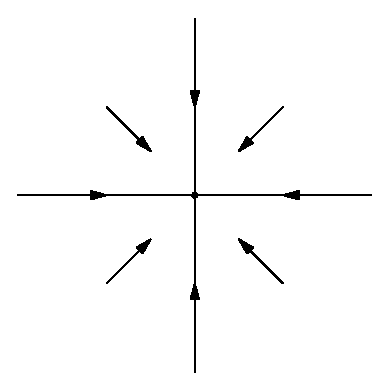
\includegraphics[width=4cm]{figure30.eps}
\caption{Stable Focus - Nullclines and Directions}
\label{figure-stable-focus-nullclines}
\end{figure}

\begin{figure}[t]
\centering
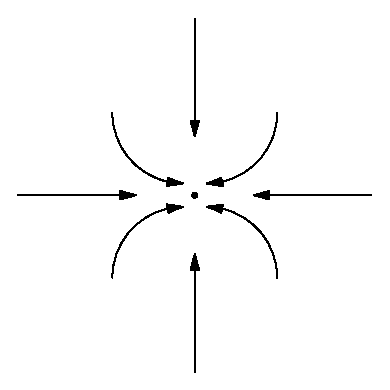
\includegraphics[width=4cm]{figure46.eps}
\caption{Stable Focus - Trajectories}
\label{figure-stable-focus-trajectories}
\end{figure}

\begin{figure}[t]
\centering
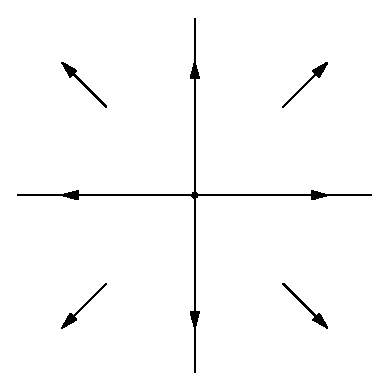
\includegraphics[width=4cm]{figure31.eps}
\caption{Unstable Focus - Nullclines and Directions}
\label{figure-unstable-focus-nullclines}
\end{figure}

\begin{figure}[t]
\centering
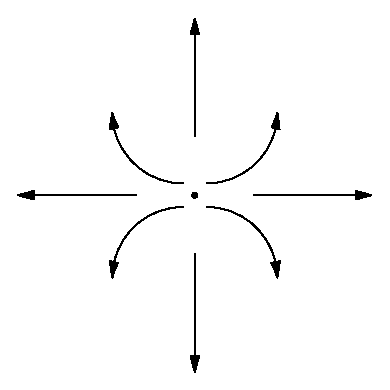
\includegraphics[width=4cm]{figure51.eps}
\caption{Unstable Focus - Trajectories}
\label{figure-unstable-focus-trajectories}
\end{figure}

\begin{figure}[t]
\centering
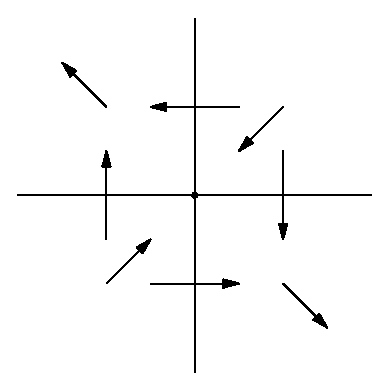
\includegraphics[width=4cm]{figure34.eps}
\caption{Saddle Point - Nullclines and Directions}
\label{figure-saddle-point-nullclines}
\end{figure}

\begin{figure}[t]
\centering
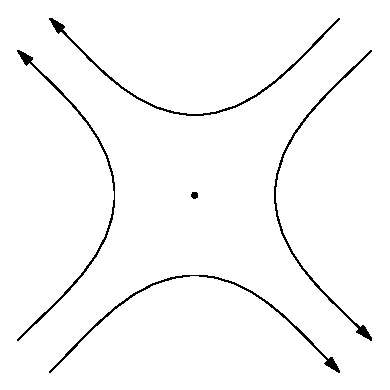
\includegraphics[width=4cm]{figure49.eps}
\caption{Saddle Point - Trajectories}
\label{figure-saddle-point-trajectories}
\end{figure}

\begin{figure}[t]
\centering
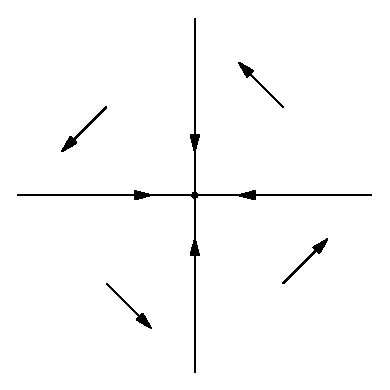
\includegraphics[width=4cm]{figure32.eps}
\caption{Stable Node - Nullclines and Directions}
\label{figure-stable-node-nullclines}
\end{figure}

\begin{figure}[t]
\centering
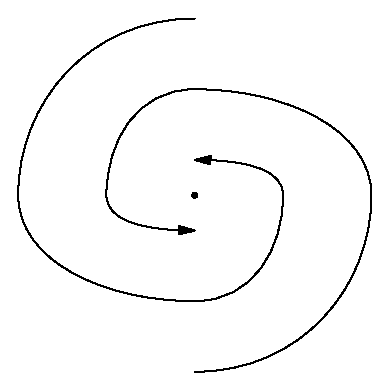
\includegraphics[width=4cm]{figure47.eps}
\caption{Stable Node - Trajectories}
\label{figure-stable-node-trajectories}
\end{figure}

\begin{figure}[t]
\centering
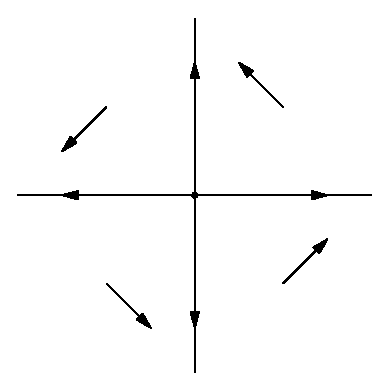
\includegraphics[width=4cm]{figure33.eps}
\caption{Unstable Node - Nullclines and Directions}
\label{figure-unstable-node-nullclines}
\end{figure}

\begin{figure}[t]
\centering
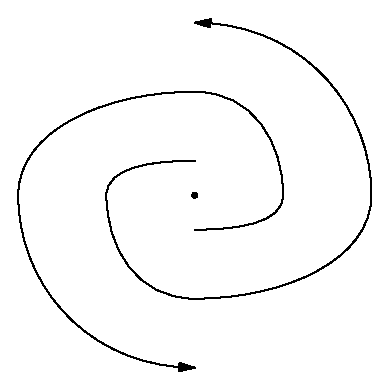
\includegraphics[width=4cm]{figure48.eps}
\caption{Unstable Node - Trajectories}
\label{figure-unstable-node-trajectories}
\end{figure}

\begin{figure}[t]
\centering
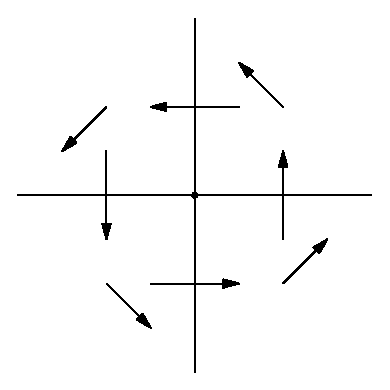
\includegraphics[width=4cm]{figure29.eps}
\caption{Centre - Nullclines and Directions}
\label{figure-centre-nullclines}
\end{figure}

\begin{figure}[t]
\centering
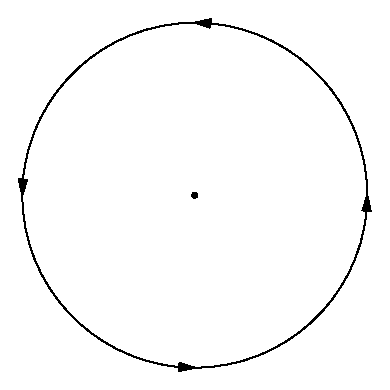
\includegraphics[width=4cm]{figure50.eps}
\caption{Centre - Trajectories}
\label{figure-centre-trajectories}
\end{figure}

\begin{example}
Let's start with Lokta-Volterra. In the above
notation, Lokta-Volterra is described by two DEs, with these
functions.
\begin{align*}
f(p,q) & = ap - bpq \\
g(p,q) & = cpq - dq 
\end{align*}
We need to graph the zero-loci of the right sides.
\begin{align*}
ap - bpq & = 0 \implies p ( a - bq) = 0\\
cpq - dq & = 0 \implies q (cp - d) = 0
\end{align*}
The loci we get are the two axes $p=0$ and $q=0$, the
horizontal line $q = \frac{a}{b}$ and the vertical line $p =
\frac{d}{c}$. There are four intersections points, $(0,0)$,
$\left(\frac{d}{c},0\right)$, $\left(0,\frac{a}{b} \right)$
and $\left( \frac{d}{c}, \frac{a}{b} \right)$. The later is
the only steady state with non-zero values, so the only
possibility for a steady state which actually involves both
species. The nullcines are shown in Figure
\ref{figure-nullclines-lokta-voltera} and the directions in Figure
\ref{figure-directions-lokta-voltera}. 

The signs of $f(p,q)$ and $g(p,q)$ give the trajectory
directions in each portion of the phase plane and on the
nullclines. We can use those directions to sketch an idea of
the trajectories of the system. For Lokta-Volterra, these
directions show something which is vaguely circular or
elliptical, as in Figure \ref{figure-trajectories-lokta-voltera}.
\end{example}

\begin{figure}[t]
\centering
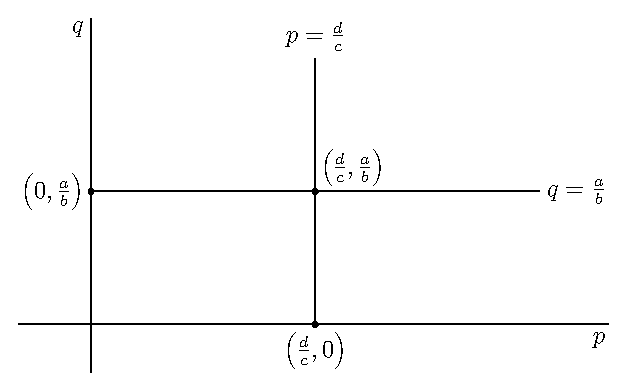
\includegraphics[width=8cm]{figure24.eps}
\caption{The Nullclines for Lokta-Voltera}
\label{figure-nullclines-lokta-voltera}
\end{figure}

\begin{figure}[t]
\centering
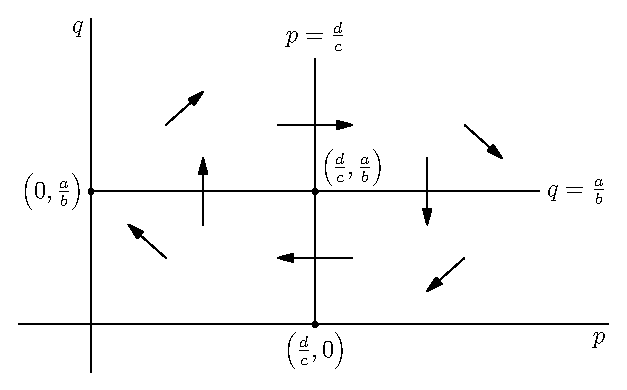
\includegraphics[width=8cm]{figure25.eps}
\caption{The Directions for Lokta-Voltera}
\label{figure-directions-lokta-voltera}
\end{figure}

\begin{figure}[t]
\centering
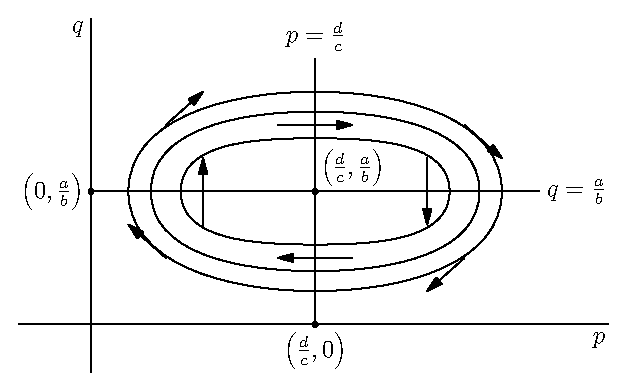
\includegraphics[width=8cm]{figure26.eps}
\caption{The Trajectories for Lokta-Voltera}
\label{figure-trajectories-lokta-voltera}
\end{figure}

\begin{figure}[t]
\centering
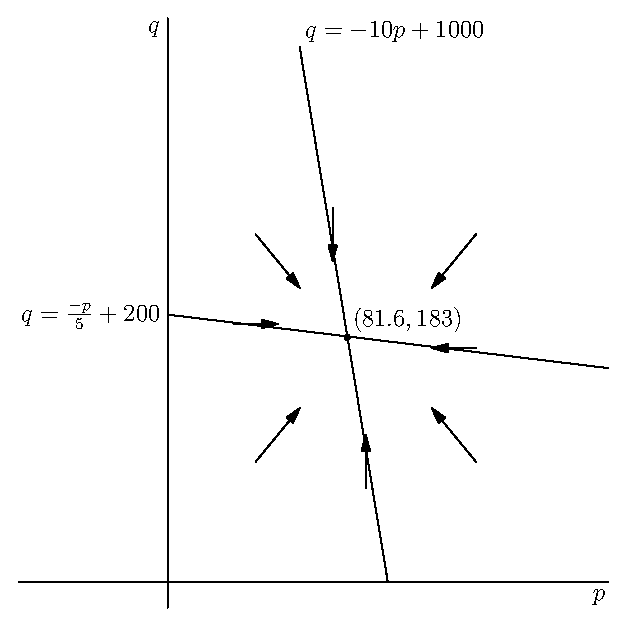
\includegraphics[width=8cm]{figure27.eps}
\caption{The Nullclines and Directions for a Competition
Example}
\label{figure-competition-example}
\end{figure}

\begin{example}
This is a competition example.
\begin{align*}
\frac{dp}{dt} & = \frac{1}{10} p\left(1- \frac{p +
\frac{1}{10}q}{100} \right) \\
\frac{dq}{dt} & = \frac{1}{5} \left(1- \frac{q + \frac{1}{5}
p}{200} \right)
\end{align*}
The zero loci of the right sides determine the nullclines.
\begin{align*}
\frac{1}{10} p\left(1- \frac{p +
\frac{1}{10}q}{100} \right) & = 0 \\
\frac{1}{5} \left(1- \frac{q + \frac{1}{5}
p}{200} \right) & = 0 
\end{align*}
Again, the axes $p=0$ and $q=0$ are nullclines. In addition,
we have the lines $p = \frac{-q}{10} + 100$ an $p - \frac{-5q}
+ 1000$. Figure \ref{figure-competition-example} shows the graph of
the nullclines with the directions of movement added.

The steady state is a stable focus. The trajectories are all
inwards towards the steady state. Therefore, we can conclude
that there is a stable equilibrium between the two competing
species and that they populations will approach this
equilibrium over time.
\end{example}

\section{Linear Systems}
\label{linear-systems}

\subsection{Qualitative Analysis}
\label{qualitative-analysis}

A linear system of two differential equations has the form 
\begin{align*}
x^\prime & = ax + by \\
y^\prime & = cx + dx. 
\end{align*}
The nullclines of a linear system are the lines $y =
\frac{-a}{b} x$ and $y = \frac{-c}{d} $. The only steady
state is $(0,0)$. The six behaviours listed in the previous
section (stable/unstable node, stable/unstable focus, saddle,
centre) are all possible. However, for linear systems,
these six cases are the \emph{only} possible cases. 

\subsection{Laplace Transforms for Linear Systems}
\label{laplace-linear-systems}

\begin{figure}[t]
\centering
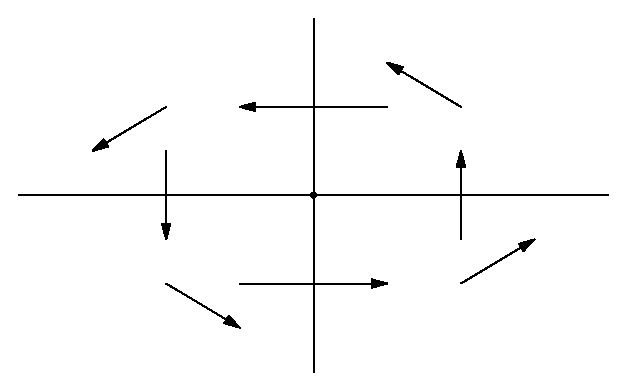
\includegraphics[width=8cm]{figure39.eps}
\caption{First Linear System Example}
\label{figure-linear-system1}
\end{figure}

\begin{example}
Let's start with a simple example. We can solve linear
systems with Laplace transforms, since the Laplace transform
will be a linear system of algebraic (not differential)
equations. We solve these with basic techniques, such as
isolating and replacing, or with linear algebra.
\begin{align*}
x^\prime & = -y \\
y^\prime & = x \\
x(0) & = 0 \hspace{1cm} y(0) = 1 \\
sX & = -Y \implies X = \frac{-Y}{s}\\
sY -1 & = X \implies sY - 1 = \frac{-Y}{S} \\
sY + \frac{Y}{s} & = 1 \\
Y & = \frac{s}{s^2+1} \\
X & = \frac{-Y}{s} = \frac{-1}{s^2+1} \\
y & = \cos t \\
x & = - \sin t \\
\end{align*}
In this case, the nullclines are simply the axes. The steady
state $(0,0)$ is a centre. Figure \ref{figure-linear-system1}
shows the nullclines and directions.
\end{example}

\begin{figure}[t]
\centering
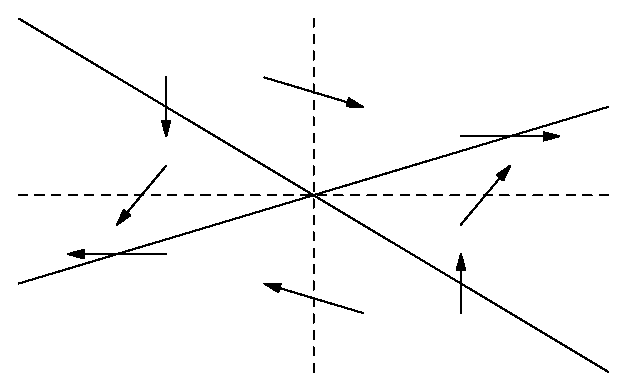
\includegraphics[width=8cm]{figure35.eps}
\caption{Second Linear System Example}
\label{figure-linear-system2}
\end{figure}

\begin{example}
\begin{align*}
x^\prime & = 2x + 2y \hspace{1cm} x(0) = 1 \\
y^\prime & = 2x - y \hspace{1.2cm} y(0) = 1 \\
sX - 1 & = 2X + 2Y \\
sY - 1 & = 2X - Y \implies X = \frac{2Y+1}{s-2} \\
sY - 2 \left( \frac{2Y+1}{s-2} \right) + Y & = 1 \\
(s+1) Y - \frac{4Y}{s-2} & = 1 + \frac{2}{s-2} \\
\left( \frac{s^2-s-6}{s-2} \right) Y & = 1 + \frac{2}{s-2} \\
Y & = \frac{s-2}{(s-3)(s+2)} + \frac{2}{(s-3)(s+2)} =
\frac{s}{(s-3)(s+2)} \\
& = \frac{\frac{2}{5}}{s+2} + \frac{\frac{3}{5}}{s-3} \\
X & = \frac{2Y+1}{s-2} = \frac{2\left( \frac{s}{(s-3)(s+2)}
\right) + 1}{s-2} = \frac{2s + s^2 - s - 6}{(s-3)(s-2)(s+2)} \\
& = \frac{(s+3)(s-2)}{(s-3)(s-2)(s+2)} 
= \frac{s+3}{(s-3)(s+2)} = \frac{\frac{6}{5}}{s-3} -
\frac{\frac{1}{5}}{s+2} \\
x & = \frac{6}{5} e^{3t} - \frac{1}{5} e^{-2t} \\
y & = \frac{2}{5} e^{-2t} + \frac{3}{5} e^{3t} 
\end{align*}
In this case, the nullclines are $y = -x$ and $y = 2x$. 
The steady state is a saddle point. The solutions are 
a mix of exponential growth and exponential decay; this mix of
growth and decay fits the expected behaviour of a saddle point.
Figure \ref{figure-linear-system2} shows the nullclines
and directions. 
\end{example}

\begin{figure}[t]
\centering
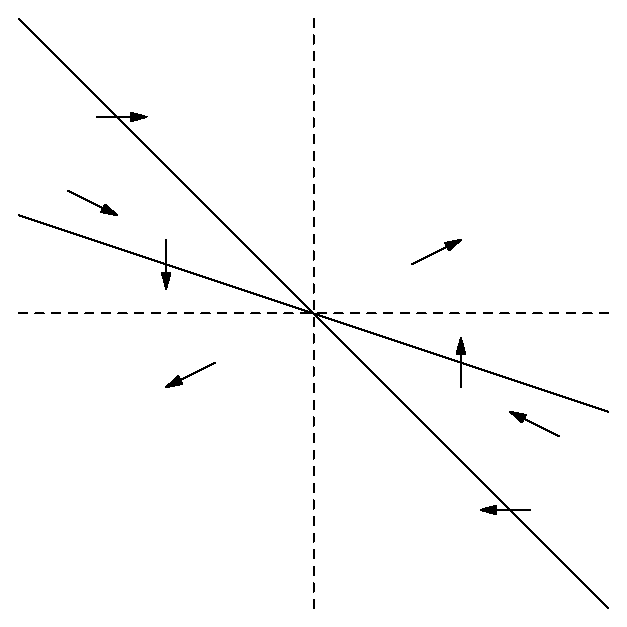
\includegraphics[width=6cm]{figure36.eps}
\caption{Third Linear System Example}
\label{figure-linear-system3}
\end{figure}

\begin{example}
\begin{align*}
x^\prime & = 2x + 3y \hspace{1cm} x(0) = 1 \\
y^\prime & = 2x + y \hspace{1.2cm} y(0) = 1\\
sX - 1 & = 2X + 3Y \\
sY - 1 & = 2X + Y \implies X = \frac{3Y+1}{s-2} \\
sY - Y - 2 \left( \frac{3Y+1}{s-2} \right) & = 1 \\
\left( \frac{s^2-3s-4}{s-2} \right) Y & = 1 + \frac{2}{s-2} \\
Y & = \frac{s-2}{(s-4)(s+1)} + \frac{2}{(s-4)(s+1)} =
\frac{s}{(s-4)(s+1)} = \frac{\frac{4}{5}}{s-4} +
\frac{\frac{-1}{5}}{s+1} \\
X & = \frac{3\frac{s}{(s-4)(s+1)} + 1}{s-2} =
\frac{3s+s^2-3s-4}{(s+1)(s-4)(s-2)} =
\frac{s^2-4}{(s+1)(s-4)(s-2)} \\
& = \frac{s+2}{(s+1)(s-4)} = \frac{\frac{6}{5}}{s-4} -
\frac{\frac{1}{5}}{s+1} \\
x & = \frac{6}{5} e^{4t} - \frac{1}{5} e^{-t} \\
y & = \frac{4}{5} e^{4t} + \frac{1}{5} e^{-t}
\end{align*}
In this case, the nullclines are $y = \frac{-2}{3}x$ and $y =
-2x$. The behaviour is again a saddle point and again we have
a mix of positive and negative exponential terms. Figure
\ref{figure-linear-system3} shows the nullclines and
directions.
\end{example}

\begin{figure}[t]
\centering
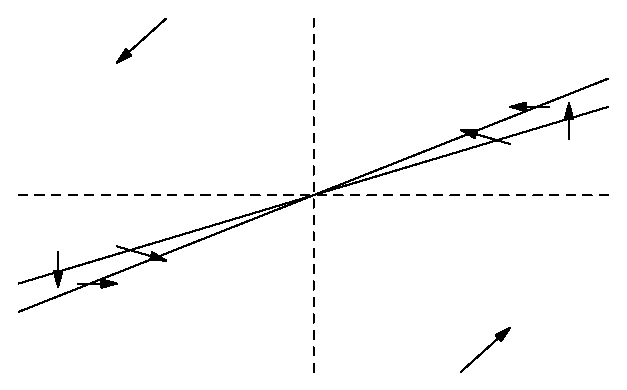
\includegraphics[width=7cm]{figure37.eps}
\caption{Fourth Linear System Example}
\label{figure-linear-system4}
\end{figure}

\begin{example}
\begin{align*}
x^\prime & = 3x - 18y \hspace{1cm} x(0) = 1\\
y^\prime & = 2x - 9y \hspace{1.2cm} y(0) = 1\\
sX - 1 & = 3X - 18Y \\
sY - 1 & = 2X - 9Y \implies X = \frac{1-18Y}{s-3} \\
sY + 9Y - 2 \left( \frac{1-18Y}{s-3} \right) & = 1 \\
\left( \frac{s^2+6s+9}{s-3} \right) Y & = 1 + \frac{2}{s-3} \\
Y & = \frac{s-3}{(s+3)^2} + \frac{2}{(s+3)^2} =
\frac{s-1}{(s+1)^2} \\
& = \frac{s}{(s+3)^2} - \frac{1}{(s+3)^2} 
= \frac{1}{s+3} - \frac{4}{(s+3)^2} \\
X & = \frac{1 - 19 \frac{s-1}{(s+3)^2}}{s-3} = 
\frac{s^2-12s+27}{(s-3)(s+3)^2}
\frac{(s-9)(s-3)}{(s-3)(s+3)^2} \\
& = \frac{s}{(s+3)^2} - \frac{1}{(s-3)^2} = \frac{1}{s+3} -
\frac{12}{(s+3)^2} \\
x & = e^{-3t} + 12 t e^{-3t} \\
y & = e^{-3t} + 4 t e^{-3t}
\end{align*}
In this case, the nullclines are $y = \frac{1}{6}x$ and $y =
\frac{2}{9}x$. The steady state is a stable focus. The
solutions are all decay terms, so they all tend to the steady
state. This doesn't really match the expected behaviour,
which looks like rotation. This is an interesting example:
the repeated factor leads to the $t e^{-3t}$ terms, which do
have more spinning motion that the general exponential terms.
This is like the critically damped case for harmonic motion:
it is very close to sinusoidal behaviour but not quite there.
It would be very easy to interpret the trajectories as
rotational; in this case, the qualitative analysis is
misleading. Figure \ref{figure-linear-system4} shows
the nullclines and directions.
\end{example}

\begin{figure}[t]
\centering
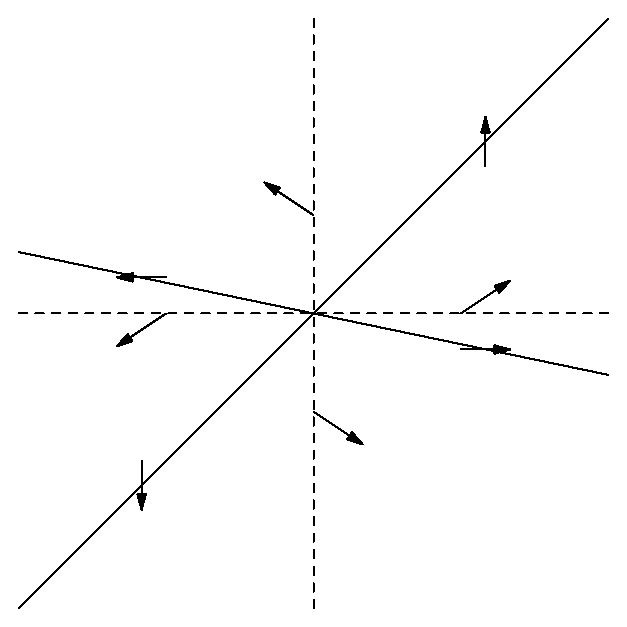
\includegraphics[width=6cm]{figure38.eps}
\caption{Fifth Linear System Example}
\label{figure-linear-system5}
\end{figure}

\begin{example}
\begin{align*}
x^\prime & = 6x - y \hspace{1.2cm} x(0) = 1 \\
y^\prime & = 5x + 4y \hspace{1cm} y(0) = 1\\
sX - 1 & = 6X - Y \\
sY - 1 & = 5X + 4Y \implies X = \frac{1-Y}{s-6} \\
(s-4)Y - 5 \left( \frac{1-y}{s-6} \right) & = 1 \\
\left( \frac{s^2-10s+29}{s-6} \right) Y & = 1 - \frac{5}{s-6}
= \frac{s-11}{s-6}\\
Y & = \frac{s-11}{s^2-10s_29} = \frac{s}{(s-5)^2+4} -
\frac{11}{(s-5)^2 + 4} \\
& = \frac{s-5}{(s-5)^2+4} - \frac{6}{(s-5)^2 + 4} \\
X & = \frac{1 - \frac{s-11}{s^2+10s+29}}{s-6} = 
\frac{s^2-11s + 40}{(s-6)(s^2-10s+29)} =
\frac{(s-6)(s-5)}{(s-6)(s^2-10s+19)} \\
& = \frac{s-5}{s^2-10s+29} = \frac{s-5}{(s-5)^2 +4} -
\frac{1}{(s-5)^2 + 4} \\
x & = e^{5t} \cos 2t - 3 e^{5t} \sin 2t\\
y & = e^{5t} \cos 2t - \frac{1}{2} e^{5t} \sin 2t
\end{align*}
In this case, the nullclines are $y = 6x$ and $y =
\frac{-5}{4}x$.  The steady state is unstable node. The
solutions have rotation in the sinusoidal terms and
exponential growth, showing the outward spiral expected from
an unstable node. Figure \ref{figure-linear-system5}
shows the nullclines and trajectories for this example.
\end{example}

\subsection{Second Order Systems}
\label{second-order-systems}

We used coupled spring as a motivating example is a linear
system. It is a second order system--in fact, it will be the
only example we'll consider of a second order system.
\begin{align*}
m_1x_1^{\prime \prime} & = - k_1x_1 + k_2(x_2 - x_1) \\
m_2x_2^{\prime \prime} & = -k_2(x_2-x_1) 
\end{align*}
Let's set the constants $m_1 = m_2 =1$, $k_1=8$ and $k_2=3$.
Let's also set the initial conditions $x_1(0) = x_1^\prime(0)
= 0$ and $x_2(0) = 1$ and $x_2^\prime(0) = 0$. These initial
condition implies that we've pushed $x_2$ away from
equilibrium. We don't have a phase-plane diagram here, since
this is a second order system. (Our phase-plane diagram
intepretation in the previous section was specific to
first-order systems.)

We solve using Laplace transforms.
\begin{align*}
x_1^{\prime \prime} + 11 x_1 - 3x_2 & = 0 \\
x_2^{\prime \prime} + 3 x_2 - 3x_1 & = 0 \\
s^2 X_1 + 11 X_1 - 3X_2 & = 0 \\
s^2 X_2 - s + 3X_2 - 3X_1 & = 0 \\
X_2 & = \frac{(s^2+11) X_1}{3} \\
(s^2+3)X_2 - 3X_1 & = s \\
(s^2+3)\left( \frac{s^2+11}{3} \right) - 3X_1 & = s \\
\frac{s^4 + 14s^2+ 33 - 9}{3} X_1 & = s \\
\frac{s^4 + 14s^2 + 24}{3} X_1 & = s \\
X_1 & = \frac{3x}{s^4 + 14s^2 + 24} = \frac{3s}{(s^2+2)(s^2+12)}
\\
X_2 & = \frac{s^2+11}{3} \frac{3s}{(s^2+2)(s^2+12)} = \frac{s^3
+ 11s}{(s^2+1)(s^2+12)} \\
X_1 & = \frac{3s}{10(s^2+2)} - \frac{3s}{10(s^2+12)} \\
X_2 & = \frac{9s}{10(s^2+2)} + \frac{s}{10(s^2+12)} \\
x_1 & = \frac{3}{10} \cos \sqrt{2}t - \frac{3}{10} \cos \sqrt{12}
t \\
x_2 & = \frac{9}{10} \cos \sqrt{2}t + \frac{1}{10} \cos \sqrt{12}
t \\
\end{align*}
Here is an adjustment of the coupled spring, where each mass
is attached to a fixed object. Then there are three springs in
total: one attaching each mass to opposite walls, and one
between them. We have a system given by Newton's laws of
motion.
\begin{align*}
m_2 x^{\prime \prime} & = -k_1 x + k_2 (y-x) \\
m_2 y^{\prime \prime} & = -k_3 y + k_2 (x-y) 
\end{align*}
We set the constants $k_1 = k_3 = 2$, $k_2 = 1$, and $m_1 =
m_2 = 1$.  For initial conditions, we set $x(0) = y(0) = 0$
and $x^\prime(0) = -1$, $y^\prime(0) = 1$. These initial
contidions show that, the masses are pushed apart equal
distances to start the system. 
\begin{align*}
x^{\prime \prime} + 3x - y & = 0 \\
y^{\prime \prime} + 3y - x & = 0 \\
s^2X + 1 + 3X - Y & = 0 \\
s^2Y - 1 + 3Y - X & 0 \\
Y & = \frac{1++X}{s^2+3} \\
(s^2+3) X - \left( \frac{1+X}{s^2+3} \right) & = - 1\\
\left( \frac{(s^2+3)(s^2+3) - 1}{s^2+3)} \right) X & = \frac{1}{s^2+3} -
1 \\
(s^4+6s^2+8)X & = -s^2-2 \\
X & = \frac{-s^2-2}{(s^2+4)(s^2+2)} = \frac{-1}{s^2+4} \\
Y & = \frac{1 + \frac{-1}{s^2+4}}{s^2+3} \\
& = \frac{s^2+4-1}{(s^2+4)(s^2+3)} \\
&= \frac{s^2+3}{(s^2+4)(s^2+3)} = \frac{1}{s^2+4} \\
x & = -\sin 2t \\
y & = \sin 2t
\end{align*}

\subsection{General Theory via Eigenvalues}
\label{general-theory}

The general linear system with two equations has the form
\begin{equation*}
x^\prime = ax + by \hspace{1cm} y^\prime = cx + dy.
\end{equation*}
We can use a 2 by 2 matrix with coefficients $a,b,c,d$ to
analyze the behaviour. We were $x$ and $y$ as the coordinates
of a vector.
\begin{equation*}
\left[ \begin{matrix} x_1^\prime \\ x_2^\prime \end{matrix}
\right] = \left[ \begin{matrix} a & b \\ c & d \end{matrix}
\right] \left[ \begin{matrix} x_1 \\ x_2 \end{matrix} \right] 
\end{equation*}
Let $v$ be an eigenvectors of the matrix and let $\lambda$ be the 
corresponding eigenvectors. 
\begin{equation*}
\left[ \begin{matrix} x_1 & x_2 \end{matrix} \right] =
e^{\lambda t} v = 
\left[ \begin{matrix} e^{\lambda t} v_1 \\ e^{\lambda t} v_1
\end{matrix} \right]
\end{equation*}
To see why this is a solution, see what happens when the
matrix acts on the vector. 
\begin{align*}
\left[ \begin{matrix} a & b \\ c & d \end{matrix} \right]
\left[ \begin{matrix} e^{\lambda t} v_1 \\ 
e^{\lambda t} v_2 \end{matrix} \right]
& = e^{\lambda t} \left[ \begin{matrix} a & b \\ c & d
\end{matrix} \right] \left[ \begin{matrix} v_1 \\ v_2
\end{matrix} \right] 
= e^{\lambda t} \lambda \left[ \begin{matrix} v_1 \\ v_2
\end{matrix} \right] 
= \left[ \begin{matrix} \lambda e^{\lambda t} v_1 \\ \lambda
e^{\lambda t} v_2 \end{matrix} \right] \\[1em]
& = \left[ \begin{matrix} \dfrac{d}{dt}e^{\lambda t} v_1
\\[1em]
\dfrac{d}{dt} e^{\lambda t} v_2 \end{matrix} \right] 
= \frac{d}{dt} \left[ \begin{matrix} e^{\lambda t} v_1 \\
e^{\lambda t} v_2 \end{matrix} \right]
\end{align*} 
If we allow for complex eigenvalues, the matrix has two
eigenvalues, wth two linearly independent eigenvectors, giving
two linearly independent solutions of this type. If the
eigenvalues are real, there are exponential growth/decay
solutions. If the eigenvalues are complex, these are
sinusoidal solutions.

\subsection{Stability via Eigenvalues}
\label{stability-eigenvalues}

Everything about a linear system can be determined by the
eigenvalues of the associated matrix. For a linear system, the
nullclines are both lines through the origin. Assuming they
are not the same line (which would make the system redundant),
the only steady state for a linear system in two equations is
$(0,0)$. As we've stated previously, there are six behaviours
at the steady state for two-dimensional linear systems: stable
and unstable foci, stable and unstable notes, centres and
saddles. We can identify each case simply by the eigenvalues.
\begin{smallitemize}
\item If both eigenvalues are real and negative, then $(0,0)$
is a stable node.
\item If both eigenvalues are real and positive, then $(0,0)$
is a unstable node.
\item If both eigenvalues are real, but one is positive and
one is negative, then $(0,0)$ is a saddle point.
\item If both eigenvalues are complex with negative real part,
then $(0,0)$ is a stable focus.
\item If both eigenvalues are complex with positive real part,
then $(0,0)$ is an unstable focus.
\item If both eigenvalues are complex and purely imaginary,
then $(0,0)$ is a centre.
\end{smallitemize}

The eigenvalues become the coefficients of the 
exponential solutions, which explains this list of
behaviours. Only when we have complex coefficients do we get
sinusoidal behaviuors, as in the spiral foci and the circular
centre. When we have real coefficients, we only get growth
and decay. The real part, in either case, is the growth or
decay term. When the real part is negative, we have decay,
which is stability. When the real part is positive, we have
growth, which is instability.

Let $M$ be the matrix and let Let $\alpha = \text{tr} M$ and $\beta
= \det M$. Then the characteristic equation of the matrix can
be written $\lambda^2 - \alpha \lambda + \beta = 0$. In addition, let
$\delta$ be the discriminant of the characteristic polynomial,
$\delta = \alpha^2 - 4\beta$. Then we can redo the previous list. 
\begin{smallitemize}
\item If $\beta > 0$, $\alpha < 0$ and $\delta > 0$ then $(0,0)$
is a stable node.
\item If $\beta > 0$, $\alpha > 0$ and $\delta > 0$, then
$(0,0)$ is an unstable node.
\item If $\beta < 0$, then $(0,0)$ is a saddle point.
\item If $\beta > 0$, $\alpha < 0$ and $\delta < 0$, 
then $(0,0)$ is a stable focus.
\item If $\beta > 0$, $\alpha> 0$ and $\delta < 0$
then $(0,0)$ is an unstable focus.
\item If $\beta > 0$, $\alpha = 0$ and $\delta < 0$
then $(0,0)$ is a centre.
\end{smallitemize}

\chapter{Partial Differential Equations}
\label{pdes}

So far, this has been a course in ordinary differential
equations, where our functions depended on one variable. The
theory of differential equations gets much more involved and
interesting when we move to functions of several variables.
The equations also get more difficult to solve; solving a
single partial differential equation (PDE) can be the work of
a whole book, a whole thesis or a whole career. For some examples,
the solutions to a particular PDE are a whole branch of
mathematics.

Many examples involve functions which depend on both position
and time. The root of modern physics is found in
differential equations that relate time derivatives to
position derivatives. There are two particularly celebrated
examples. 

\begin{example}
The Navier-Stokes equation is the
fundamental equation of fluid dynamics.
There are several forms, but we'll state the form for
incompressible flows. In this equation, $u$ is the field
describing the fluid flow as a function on $x,y,z,t$ (position
and time), $\nabla$ is a differential operator, $P$ is the
pressure of the fluid, $\rho$ is the density of the fluid, and
$\nu$ is the viscosity of the fluid. 
\begin{equation*}
\frac{\del u}{\del t} + u \cdot \nabla u = - \frac{\nabla
P}{\rho} + \nu \nabla^2 u.
\end{equation*}
\end{example}

\begin{example}
The Schrodinger equation
is the fundamental PDE in quantum mechanics (at least in
its early versions). In the Schrodinger equation, $\Psi$ is
the wave function which describes the probabilities of
measurements in a physical system, $\imath$ is the familiar
complex number, $\hbar$ is a constant, $m$ is mass and $V$ is
a potential. This is the one-dimensional version, so $\Psi$ depends on
$x$ and $t$.
\begin{equation*}
\imath \hbar \frac{\del \Psi}{\del t} = \frac{-\hbar^2}{2m}
\frac{\del^2 \Psi}{\del x^2} + V(x) \Psi
\end{equation*}
\end{example}

\section{The Heat Equation}
\label{heat-equation}

In our very short investigation of PDEs, we will look at two
equations. The first is the heat equation. It concerns a
function $u(x,t)$ which depends on position and time.
$u(x,t)$ measures the heat in a one-dimensional object (usually
a rod, rail, wire, stick or something similar). The heat varies in
position along the object as well as in time. We let $x \in [0,l]$
where $l$ is the length of the rod. For convenience (by
choosing appropriate units), we will set $l = \pi$.

The question we want to ask is this: how does the heat
distribution along the rod develop over time? What happens to
the heat at various positions and times? Where does the heat
flow, increase, decrease and diffuse? The heat
equation tries to answer this question. 

Thermodynamics says that heat wants to diffuse. Diffusion is
the equalizing of differences, so the greater the difference
in heat, the greater the inclination for difussions. How do
we measure this? The measurement must be local, since heat
cannot jump discontinuously. The local description that
measures this heat difference is the concavity of the
function. Moreover, concave down regions want to equalize
downward and concave up regions want to equalize upwards, as
in Figure \ref{figure-heat-equation}.
Therefore, the heat diffusion should be proportional to the
concavity with a positive proportionality constant.

\begin{figure}[t]
\centering
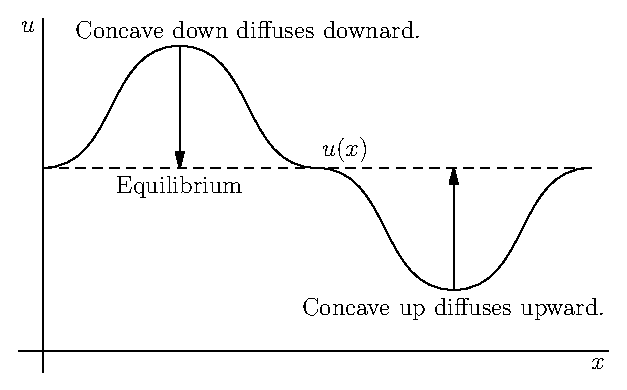
\includegraphics[width=12cm]{figure40.eps}
\caption{Concavity and Heat Diffusion}
\label{figure-heat-equation}
\end{figure}

We translate these thermodynamic realities into a partial
differential equation. The second derivative in position
measure concavity and the first derivative in time measures the
change in heat resulting from the diffusion. The above set-up
shows that these should be proportional to each other. Let $k$
be a positive number.
\begin{equation*}
\frac{\del u}{\del t} = k \frac{\del^2 u}{\del x^2}.
\end{equation*}
This is called the heat equation. Though we've defined it by
talking about heat, it is a very general equation and applies
to any system that involves diffusion. It is sometimes also
called the diffusion equation.

\subsection{Initial and Boundary Conditions}
\label{initial-boundary-conditions}

With ordinary differential equations, we needed initial
conditions to get a particular solution. The same it true
with PDEs, but the initial assumptions are more complicated.
At a specific time, say $t=0$, the function $u(x,0)$ is still
a function of $x$. Our initial condition, then, is an entire
function: $u(x,0) = f(x)$.

The initial condition determines the situation at the starting
time. However, we also need to control the behaviour of
position. For position, instead of initial conditions, we have
boundary conditions.  These tell us the behaviour of the
system at its boundaries.  For the heat equation on a rod, we
have $x\in [0,\pi]$, so the boundary contitions are
determination of $u(0,t)$ and $u(\pi,t)$. These themselves can
be functions of $t$. However, for our purposes, we'll set the
boundary contitions to be constant. If we set the units of
temperature reasonably, we can have $u(0,t) = u(\pi,t) = 0$.
These boundary condition mean that we have a constant
temperature at both ends of the rod at all moments in time.
(In physical terms, there are perfect instantaneous heat-sinks
at each end of the rod which equalize it to the ambient
temperature of zero). 

\subsection{Solving the Heat Equation}
\label{sovling-heat-equation}

The method of approach we use to solve the equation is a
common one for PDE and is called \emph{seperation of
variables}. We make the assumption (eventually justified!)
that we can pull apart the two variables, $x$ and $t$, and
deal with the seperately. We assume that $u$ is a product of
two single variables functions.
\begin{equation*}
u(x,t) = T(t) X(x).
\end{equation*}
Like all of our assumptions about DEs, we simply put this back
into the equation.
\begin{align*}
\frac{\del^2 u}{\del x^2} & = X^{\prime \prime}(x) T(t) \\
\frac{\del u}{\del t} & = T^{\prime}(t) X(x) \\
k X^{\prime \prime} T(t) & = X(t) T^\prime(t) \\
\frac{X^{\prime \prime}(x)}{X(x)} & = \frac{1}{k}
\frac{T^\prime(t)}{T(t)} 
\end{align*}
We bring all the terms involving $x$ to one side and
all those involving $t$ to the other. Since the left is equal
to the right and they involve different variables, both sides
must be constant. Let's call this constant $\alpha$. This
completes the seperation of variables, giving us two
ordinary differential equations.
\begin{align*}
\frac{X^{\prime \prime}(x)}{X(x)} & = \alpha \\
\frac{1}{k} \frac{T^\prime(t)}{T(t)} & = \alpha
\end{align*}
Now, to solve the heat equation with seperation of variables,
we solve these two ODEs seperately. The $T$ solutions are easy.
\begin{equation*}
T^\prime(t) = \alpha k T(t) \implies T(t) = T(0) e^{\alpha kt}
\end{equation*}
We have written the initial constant as $T(0)$. The time
function is just exponential growth/decay, but $X$ solutions
depend more carefully on the boundary conditions. 

\begin{figure}[t]
\centering
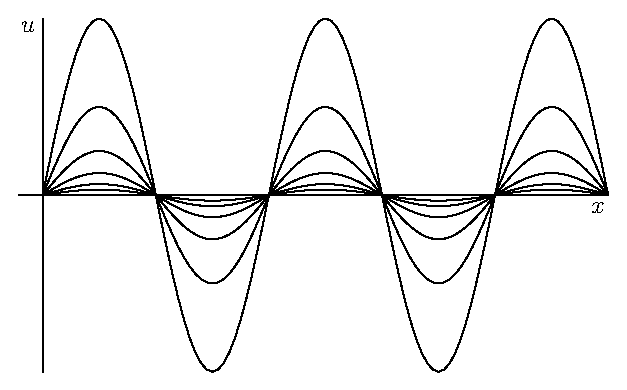
\includegraphics[width=12cm]{figure41.eps}
\caption{Seperated Solution with $n=5$ at Various Points in
Time.}
\label{figure-seperable-solution1}
\end{figure}

The $X$ equation is a second order linear equation: $X^{\prime
\prime}(x) - \alpha X(x) = 0$. If $\alpha > 0$ then we expect
exponential solutions $X(x) = c_1 e^{\alpha x} + c_2e^{\alpha
x}$. However, the boundary conditions apply. $X(0) = X(\pi) =
0$ implies that $c_1 = c_2 = 0$; the only solution here is the
trivial solution $X(x) = 0$.  Therefore, to get solutions that
actually mean somthing, $\alpha$ cannot be positive. If
$\alpha = 0$ then we get $X = Ax + B$. Again, the boundary
conditions give $A=B=0$, so we only get the zero solution.
Therefore, only $\alpha < 0$ gives interesting solutions. 

(This $\alpha < 0$ also effects the $T$ solutions, which relied
on the same $\alpha$. The fact that $\alpha < 0$ means that
the $T$ solutions must be decaying exponentials instead of
growing exponentials. This is physically expected, since over
time the heat should diffuse.)

Let $\alpha = -n^2$ for $n > 0$ a real number. From our study
of second order linear equations, the solutions are
\begin{equation*}
X(x) = A \cos nx + B \sin nx.
\end{equation*}
Again, we go back to the boundary conditions. $X(0) = 0$
implies $A=0$, so we are left with $X(x) = B \sin nx$. Then
$X(\pi) = 0$ implies $B \sin n\pi = 0$ which is only satisfied
if $n \in \NN$. In conclusion, matching the boundary
conditions means that the only possible $X$ solutions are
$X(x) = B \sin nx$ for $n \in \NN$ (and the zero solution). 

Then we put the solutions together.
\begin{equation*}
u(x,t) = T(0) e^{-n^2kt} \sin (nx) 
\end{equation*}

In these solutions, we see sine waves decaying over time. The
integer $n$ gives the number of osscilations of the wave in
on the rod, and the exponential terms give a decay in
amplitude over time. Figure \ref{figure-seperable-solution1} shows the
decay of a simple sine wave with $n=5$.

Now we consider the initial condition $u(x,0) = f(x)$. For
each $n$, the seperable solution is a sine wave $\sin
(nx)$. This is great if $f(x)$ happened to be such a sine
wave, but we would like the theory to work with more general
initial conditions. The key observation here is that the heat
equation is linear: if we have two solutions to the
heat equation, their sum is also a solution. Therefore, we
could add up these seperable solutions. For example, a
possible solution could be 
\begin{equation*}
u(x,t) = 4e^{-9kt} \sin 3t + 6e^{-25kt} \sin 5t.
\end{equation*}
This isn't strictly seperable anymore, but it is the sum of
seperable pieces. (This justifies the original assumption! We
don't get all possibility as seperable solutions, but we will
get all reasonable solutions as the \emph{sum} of various
seperable pieces.) The initial value $u(x,0)$ also isn't a
simple sine wave anymore, since it is the function $f(x) =
4\sin 3t + .6 \sin 5t$. Figure \ref{figure-seperable-solution2} shows
the decay of this initial condition.

\begin{figure}[t]
\centering
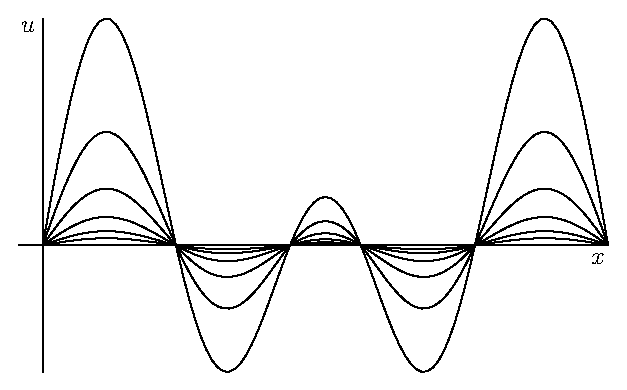
\includegraphics[width=12cm]{figure42.eps}
\caption{Decay of the Solution with Initial Condition $f(x) =
4 \sin 3t + 6 \sin 5t$}
\label{figure-seperable-solution2}
\end{figure}

In theory, we could add any number of the seperable solutions
together. Therefore, in full generality, a solution could
look like an arbitrary sum.
\begin{equation*}
u(x,t) = \sum_{n=1}^\infty T_n(0) e^{-n^2kt} \sin (nx) 
\end{equation*}
This is a series solution, but the series has $\sin nx$
instead of $x^n$ as the series terms. We try to match our
initial condition $u(x,0) = f(x)$ with this series.
\begin{equation*}
u(x,0) = \sum_{n=1}^\infty T_n(0) \sin (nx) = f(x) 
\end{equation*} 
As long as we can find coefficients $T_n(0)$ that make this
series work, we can solve the heat equation. That leads to
this question: which functions $f(x)$ can be expressed as a
series in $\sin (nx)$ in this way? Once we know that, we can
have a full, general solution to the heat equation (with
constant zero boundary conditions).

\section{Fourier Series}
\label{fourier-series}

The answer to the question at the end of the previous section
is very positive: most functions can, in fact, be approximated
by a series with term $\sin nx$. These series are called Fourier
series and we'll spend the current section defining and
investigating them.

\subsection{Series and Bases for Functions}
\label{bases}

The series in the previous section only involved sine
functions, but the general Fourier series involves both sine
and cosine.

\begin{defn}
Let $a_n$ and $b_n$ be real numbers. A \emph{Fourier series}
is a series of the form
\begin{equation*}
f(x) = \frac{a_0}{2} + \sum_{n=1}^\infty a_n \cos (nx) +
\sum_{n=1}^\infty b_n \sin (nx).
\end{equation*}
\end{defn}

In general, function as series can be consider a sums over a
particular basis. For Taylor series, the basis was the set of
monomials: $x^n$ for $n \in \NN$. A Taylor series is an
attempt to write a general function as a sum of these
monomials.  For Fourier series, the is $\{ 1, \cos nx, \sin nx
\}$ for $n \in \NN$. 

In a Fourier series, we can split the basis into two pieces:
the sine pieces and the cosine pieces (including the constant
$1$ in the later). If we restrict to only one piece, we could
form a Fourier sine series or Fourier cosine series. The sine
pieces are all odd functions; therefore, a Fourier sine series
must be an odd function. Likewise, the cosine pieces
(including the constant) are all even functions, so a Fourier
cosines series must be an even function. 

If we have a general function $f$, we can write $f = f_+ +
f_-$ where $f_+$ is even and $f_-$ is odd. The pieces are easy
to define: $f_+ = \frac{1}{2} (f(x) + f(-x))$ and $f_- =
\frac{1}{2} (f(x) - f(-x))$. If $f$ has a Fourier series, then
$f_-$, the odd piece, will have a Fourier sine series and
$f_+$, the even piece, will have a Fourier cosine series. The
heat equation, since we insisted on starting at $(0,0)$ and
only considering positive values, only needs one of the two
types. Since sines arose in the solution, we'll assume the
solution to the heat equation is odd and rely on Fourier sine
series.

\subsection{Scope of Fourier Series}
\label{fourier-scope}

The good news about Fourier series is that they cover a large
family of functions. 

\begin{thm}
If $f$ is periodic and piecewise continuous on $\RR$ with
period $2T$, the there exists $a_n$ and $b_n$ such that 
\begin{equation*}
f(x) = \frac{a_0}{2} + \sum_{n=1}^\infty a_n \cos \left(
\frac{n\pi x}{T} \right) + \sum_{n=1}^\infty b_n \sin \left(
\frac{n\pi x}{T} \right).
\end{equation*}
\end{thm}

If we don't want to work with periodic functions, we can
simply look at any piecewise-continuous function defined on
$[0,2T)$, thinking of it as one period, and find a Fourier
series for it. (This method works for any finite intervals.)

\begin{thm}
If $f$ is piecewise continuous on $[0,2T)$
then there exists $a_n$ and $b_n$ such that 
\begin{equation*}
f(x) = \frac{a_0}{2} + \sum_{n=1}^\infty a_n \cos \left(
\frac{n\pi x}{T} \right) + \sum_{n=1}^\infty b_n \sin \left(
\frac{n\pi x}{T} \right).
\end{equation*}
\end{thm}

Therefore, we can use Fourier series to approximate any
piecewise continuous function on a bounded interval, which is
a very large class of functions.

\subsection{Properties of Fourier Series}
\label{fourier-properties}

When we talked about the Lagrange polynomials, we derived a
very nice orthogonality property for them. As opposed to the
ordinary monomials $x^n$, the Lagrange polynomials were
pair-wise orthogonal, using integration on $[-1,1]$ as the
inner product. When we find a basis for a type ofseries, it
is very convenient for integration if the basis functions are
orthogonal. (Like in linear algebra, an orthogonal basis is
always easy to use). 

Fourier series terms have wonderful orthogonality properties. For
convenience, these properties are stated for the period $T =
2\pi$. 

\begin{prop}
Let $n, m \in \NN$, with the possibility that $m=0$ to
account for the constant term.
\begin{align*}
\int_{-\pi}^{\pi} \cos (mx) \cos (nx) dx & = \pi \delta_{mn} \\
\int_{-\pi}^{\pi} \sin (mx) \sin (nx) dx & = \pi \delta_{mn} \\
\int_{-\pi}^{\pi} \cos (mx) \sin (nx) dx & = 0
\end{align*}
Therefore, all the Fourier basis functions are orthogonal
under the scalar product given by integration on $[-\pi,\pi]$. 
\end{prop}

\begin{proof}
For the proof, we use the trig identities for products
of $\sin$ and $\cos$, such as 
\begin{equation*}
\cos A \cos A = \frac{1}{2} \left( \cos(A-B) + \cos (A+B)
\right).
\end{equation*}
We only show the proof of the first of the three statements.
\begin{align*}
\int_{-\pi}^{\pi} \cos (mx) \cos (nx) dx & = \frac{1}{2}
\int_{-\pi}^\pi \cos ((m-n)x) + \cos((m+x)x)dx \\
& = \frac{1}{2} \left. \left[ \frac{-\sin((m-n)x)}{m-n} -
\frac{-\sin((m+n)x)}{m+n} \right] \right|_{-\pi}^{\pi} =
0 \hspace{2cm} \text{if } m \neq n \\
& = \frac{1}{2} \int_{-\pi}^\pi 1 + \cos 2m dx \\
& = \frac{1}{4} \left. \left( \frac{-\sin mx}{m} \right) +
\frac{x}{2} \right|_{\pi}^\pi = 0 + \frac{2\pi}{2} = \pi
\hspace{2cm} \text{if } m = n
\end{align*}
\end{proof}

For Taylor series, we had convenient properties for the
calculus of the series and the calculation of coefficients.
Similar properties exist for Fourier series. If we know a
series is convergent, we can integrate and differentiate
term-wise. (Not that differentiation and integration change
a Fourier sine series into a Fourier cosine series and
vice-versa.)

A method for the the calculation of coefficients comes from 
the orthogonality property. Assume that $f(x)$ is
expressed as a Fourier series.
\begin{equation*}
f(x) = \frac{a_0}{2} + \sum_{n=1}^\infty a_n \cos (nx) +
\sum_{n=1}^\infty b_n \sin (nx)
\end{equation*}
Then we can calculate an integral.
\begin{align*}
\int_{-\pi}^\pi f(x) \cos mx dx & = 
\int_{-\pi}^\pi \frac{a_0}{2} dx + \int_{-\pi}^\pi \sum_{n=1}^\infty
a_n \cos (nx) dx +
\int_{-\pi}^\pi \sum_{n=1}^\infty b_n \sin (nx) dx \\
& = 0 + \sum_{n=1}^\infty a_n \pi \delta_{mn} +
\sum_{n=1}^\infty 0 \\
& = a_n \pi 
\end{align*}
The integral calculates the coefficient $a_n$. Similarly, the
constant coefficient $a_0$ and the sine coefficients are
calculated by integrals. This gives a general result for
calculating Fourier coefficients, for $n \in \NN$.

\begin{prop}
If $f$ is expressed as a Fourier series, then the Fourier
coefficient $a_n$ and $b_n$ satisfy these equations.
\begin{align*}
a_n & = \frac{1}{\pi} \int_{-\pi}^\pi f(x) \cos nx dx \\
b_n & = \frac{1}{\pi} \int_{-\pi}^\pi f(x) \sin nx dx \\
a_0 & = \frac{1}{\pi} \int_{-\pi}^\pi f(x) dx
\end{align*}
\end{prop}

\begin{example}
Let's express $f(x) = x$ on $(-\pi, \pi)$ as a
Fourier series. Notice that $f(x)$ is odd, so only sine terms
are expected. We calculate the coefficients of the sine terms
with integrals.
\begin{align*}
b_n & = \frac{1}{\pi} \int_{-\pi}^\pi f(x) \sin nx dx \\
& = \frac{1}{\pi} \int_{-\pi}^\pi x \sin nx dx \\
& = \frac{1}{\pi} \left. \left( \frac{-x\cos nx}{n} \right)
\right|_{-\pi}^\pi + \int_{-\pi}^\pi \frac{\cos nx}{n} dx \\
& = \frac{1}{\pi} \left( \frac{ -\pi \cos n \pi }{n} + \frac{\pi
\cos (-n\pi}{n}) + 0 \right) \\
& = \frac{1}{\pi} \left( \frac{-2\pi}{n} \right) \cos n\pi =
\frac{-2(-1)^n}{n} = (-1)^{n+1}\ \frac{2}{n}\\
x & = 2 \sum_{n=1}^\infty \frac{(-1)^{n+1}}{n} \sin nx
\end{align*}
\end{example}

\subsection{Finishing the Heat Equation Solution}
\label{finishing-heat-equation}

If we go back to the heat equation, the initial conditions where
$u(x,0) = f(x)$ for some given function $f$ on $[0, \pi]$ with
$f(0) = f(\pi) = 0$. When $t=0$, we wrote that 
\begin{equation*}
f(x) = \sum_{n=1}^\infty T_n \sin (nx).
\end{equation*}
The coefficients $T_n$ in the full solution to the heat
equation must be the Fourier coefficients of the initial 
function $f(x)$. Now we know how to calculate these coefficients.
Since this is a sine series, we expect that $f$ is odd, and we
extend it to $(-\pi,\pi)$ as an odd function. Then we
integrate to find the coefficients.
\begin{equation*}
T_n = \frac{2}{\pi} \int_0^\pi f(x) \sin nx dx
\end{equation*}
Therefore, the full solution to the heat equation, with
initial conditions $f(t)$ and boundary conditions $u(0,t) =
u(\pi,t) = 0$, is
\begin{equation*}
u(x,t) = \frac{2}{\pi} \sum_{n=1}^\infty \left[ \int_0^\pi f(x)
\sin nx) dx \right] e^{-kn^2t} \sin (nx).
\end{equation*}

\section{Boundary Conditions for the Heat Equation}
\label{heat-equation-boundary}

\begin{figure}[t]
\centering
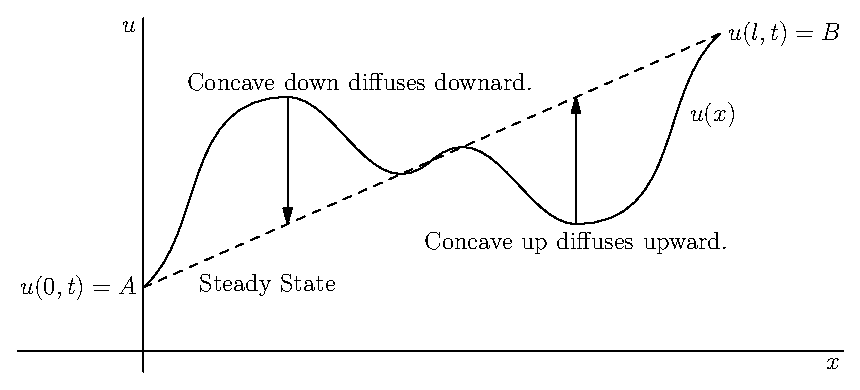
\includegraphics[width=12cm]{figure43.eps}
\caption{Diffusion to a Linear Steady State}
\label{figure-diffusion1}
\end{figure}

The general solution in this case is the sum of this steady
There are many pieces to the setup and solution of a PDE. In
what we've done so far for the heat equation, we allowed a
nearly-arbitrary initial conditions, since any function which
has a Fourier series satisfied. However, our boundary
conditions were very restrictive. We can get more complicated
situations if we relax the boundary conditions. A small
increase in complexity comes from constant but non-equal
boundary conditions: $u(0,t) = A$ and $u(\pi,t) = B$ for some
constants $A$ and $B$. This is a situation where we will keep
the ends of the rod at constant temperature, but those
temperatures need not be the same.

In this case, seperation of variables when $\alpha = 0$
implies that $X(x)$ must be a linear function. Matching the
boundary contions (with a rod of length $\pi$) means that
$X(x) = \frac{B-A}{\pi}x + A $.  This is called the
steady-state solution and it is the base case of the
situation. (For the previous case with zero boundary
conditions, the steady state solution was just $X(x) = 0$.)
The steady-state solution is the solution to which we want the
situaiton to diffuse; it is the resting case. With non-equal
boundary conditions, the steady state involves a heat flow
along the rod, from the warmer end to the cooler. A
complicated initial heat-situation will diffuse and reduce to a
straight-line distribution between the tempeartures at each
end as show in Figure \ref{figure-diffusion1}.

state with our previous solutions. The linearity of the
system means that the solution with both boundary conditions
set to $0$ can simply be added to this steady state to give
the general solution.
\begin{equation*}
u(x,t) = \frac{2}{\pi} \sum_{n=1}^\infty T_n e^{-kn^2t} \sin (nx) 
\end{equation*}
The calculation of the Fourier coefficients $T_n$, however,
needs an adjustment. We need to shift the function
back to a 0-equilibrium situation to repeat the result of the
previous section. With that shift, the integral that
calculates the coefficient is 
\begin{equation*}
T_n = \frac{2}{\pi} \int_0^\pi \left( f(x) - \frac{B-A}{\pi} x
- A \right) \sin nx dx.
\end{equation*}

\begin{figure}[t]
\centering
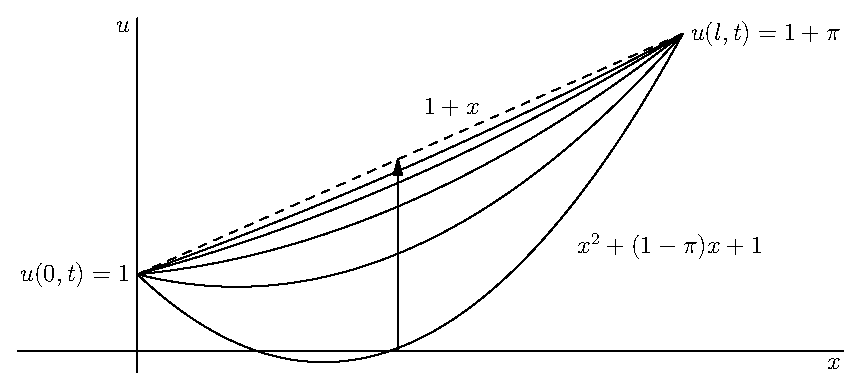
\includegraphics[width=12cm]{figure44.eps}
\caption{Heat Equation Examples with Initial Conditions $f(x)
= x^2 + (1-\pi)x + 1$}
\label{figure-diffusion2}
\end{figure}

\begin{example}
We use an example to see what this looks like with explicit
numbers. This example is from Roberts and Marion.  Set the
boundary contidions to be $u(0,t) = 1$ and $u(\pi, t) = 1 +
\pi$ and the initial condition $u(x,0) = x^2 + (1-\pi)x + 1$.
The steady state solution is the line $u = x+1$. We calculate
the Fourier coefficients. 
\begin{align*}
T_n & = \frac{2}{\pi} \int_0^\pi (x^2 - \pi x) \sin nx =
\frac{2}{\pi} \int_0^\pi x^2 \sin nx 
- 2 \int_0^\pi x\sin nx \\
& = \frac{2}{\pi} \left( \left. \frac{-x^2 \cos nx}{n}
\right|_0^\pi + \frac{2}{n} \int_0^\pi x \cos nx \right) -
2 \left( \left. \frac{-x \cos nx}{n} \right|_0^{\pi} +
\int_0^{\pi} \cos nx dx \right) \\
& = \frac{2}{\pi} \left( \frac{-\pi^2 \cos n\pi}{n} +
\left. \frac{2}{n} \frac{x \sin nx}{n} \right|_0^\pi -
\frac{2}{n^2} \int_0^\pi \sin nx \right) - 2 \left(
\frac{2\pi}{n} + \left. \frac{\sin nx}{n} \right|_0^{\pi}
\right) \\
& = \frac{2}{\pi} \left( \frac{\pi^2 (-1)^{n+1}}{n} + 0 + \left.
\frac{2\cos nx}{n^3} \right|_0^\pi \right) - \frac{4\pi}{n} -
0\\
& = \frac{2}{\pi} \left( \frac{\pi^2 (-1)^{n+1}}{n} +
\frac{2(-1)^n}{n^3} - \frac{2}{n^3} - \frac{2\pi^2}{n}\right) \\
& = \frac{2n^2 \pi^2 (-1)^{n+1} + 2\pi (-1)^n - 2\pi - 4\pi
n^2 }{\pi n^3}
\end{align*}
The general solution is
\begin{equation*}
u(x,t) = 1 + x + \sum_{n=1}^\infty \left[ \frac{2n^2 \pi^2
(-1)^{n+1} + 2\pi (-1)^n - 2\pi - 4\pi n^2}{\pi n^3} \right] e^{-kn^2t}
\sin (nx).
\end{equation*}
Figure \ref{figure-diffusion2} shows this situation.
\end{example}

\end{document}
